% \iffalse meta-comment
%
% Copyright (C) 2014 by Pascal Richter, Elena Botoeva, Richard Barnard, Dirk Surmann
% -----------------------------------
%
% This file may be distributed and/or modified under the
% conditions of the LaTeX Project Public License, either
% version 2.0 of this license or (at your option) any later
% version. The latest version of this license is in:
%
%    http://www.latex-project.org/lppl.txt
%
% and version 2.0 or later is part of all distributions of
% LaTeX version 2014/01/15 or later.
%
% \fi
%
% \iffalse
%<*driver>
\ProvidesFile{tikzposter.dtx}
\documentclass{ltxdoc}
\usepackage{subfigure}
\usepackage{tikz}
\usepackage{fancyvrb,hyperref}
\usepackage{setspace}
\EnableCrossrefs
\CodelineIndex
\RecordChanges
\OnlyDescription
\definecolor{macro}{HTML}{1B1BB3}
\definecolor{option}{HTML}{009999}
\definecolor{color}{HTML}{00CC00}%62E200}
\definecolor{style}{HTML}{E60042}
\definecolor{value}{HTML}{FF7400}
\definecolor{node}{HTML}{6F0AAA}
\newcommand{\mmacro}[1]{{\color{macro} {#1}}}
\newcommand{\moption}[1]{\textcolor{option}{#1}}
\newcommand{\mcolor}[1]{\textcolor{color}{#1}}
\newcommand{\mstyle}[1]{\textcolor{style}{#1}}
\newcommand{\mvalue}[1]{\textcolor{value}{#1}}
\newcommand{\mnode}[1]{\textcolor{node}{#1}}
\begin{document}
  \DocInput{tikzposter.dtx}
\end{document}
%</driver>
% \fi
% 
% \CheckSum{0}
%
% \CharacterTable
%  {Upper-case    \A\B\C\D\E\F\G\H\I\J\K\L\M\N\O\P\Q\R\S\T\U\V\W\X\Y\Z
%   Lower-case    \a\b\c\d\e\f\g\h\i\j\k\l\m\n\o\p\q\r\s\t\u\v\w\x\y\z
%   Digits        \0\1\2\3\4\5\6\7\8\9
%   Exclamation   \!     Double quote  \"     Hash (number) \#
%   Dollar        \$     Percent       \%     Ampersand     \&
%   Acute accent  \'     Left paren    \(     Right paren   \)
%   Asterisk      \*     Plus          \+     Comma         \,
%   Minus         \-     Point         \.     Solidus       \/
%   Colon         \:     Semicolon     \;     Less than     \<
%   Equals        \=     Greater than  \>     Question mark \?
%   Commercial at \@     Left bracket  \[     Backslash     \\
%   Right bracket \]     Circumflex    \^     Underscore    \_
%   Grave accent  \`     Left brace    \{     Vertical bar  \|
%   Right brace   \}     Tilde         \~}
%
% \changes{v1.0}{2012/09/15}{Initial version}
%
% \GetFileInfo{tikzposter.cls}
% \def\filedate{2014/01/15}
% \def\fileversion{v2.0}
% \def\fileinfo{LaTeX Poster Class with TikZ}
%
% \DoNotIndex{\#,\$,\%,\&,\@,\\,\{,\},\^,\_,\~,\ }
% \DoNotIndex{\@ne}
% \DoNotIndex{\advance,\begingroup,\catcode,\closein}
% \DoNotIndex{\closeout,\day,\def,\edef,\else,\empty,\endgroup}
%
% \title{The \textsf{tikzposter} class \thanks{This document corresponds to \textsf{tikzposter}~\fileversion, dated~\filedate.}}
% \author{Pascal Richter, Elena Botoeva, Richard Barnard, Dirk Surmann \\[1ex] \texttt{tikzposter@mathcces.rwth-aachen.de} \\ \url{https://bitbucket.org/surmann/tikzposter/wiki/}}
%
% \maketitle
%
% \begin{abstract}
%   This document class aims to provide a simple way of using LateX and TikZ for
%   generating good looking scientific posters.
% \end{abstract}
%
% \renewcommand{\baselinestretch}{0.75}
% \tableofcontents
% %\renewcommand{\baselinestretch}{1}
%
% \section{Introduction}
% The \textsf{tikzposter} document class file may be used to simplify formatting and generating scientific posters
% in the \textsf{.pdf} format.  It uses the TikZ package to generate a poster layout.  % The poster is formed by a series of blocks against a background in a sequence of aligned columns.
% The purpose of the class is to reduce the level of formatting by automatically setting spacing between
% blocks in the poster as well as their lengths.  The user has control over the width of the columns.
% Due to the class' reliance on TikZ, only \textsf{.pdf} output is supported.  This document explains the
% formatting options available and how to easily create a basic block layout.
%
% To start with the class, the user can look at either the template file included with the class |tikzposter-template.tex| (also shown in Section \ref{sec:template}) which provides a template, the minimal working example shown in Section \ref{sec:usage}, or the example file |tikzposter-example.tex|.  The last file illustrates various formatting options available.
% In Section \ref{sec:docclass}, the |\documentclass| is described.
% Inside of the |document| environment, the title is created by the use of one of the title block commands
% and columns of aligned blocks are then created; the various commands are described in the subsections of Section \ref{sec:postercontents}.
% If you want to alter the appearance of the poster, the various ways of doing this are explained in Section \ref{sec:posterlayout}.  Finally, the Appendix (Section \ref{sec:appendix}) lists useful variables for those who want to further customize the appearance of the posters.
%\vspace{12pt}
%
%\noindent\textbf{Required packages:}  The class uses \LaTeX2e and the following required packages:
% |tikz|, |calc|, |ifthen|, |ae|, |xstring|, |etoolbox|, |xkeyval|.  
%\vspace{12pt}

% \noindent\textbf{Changes from previous versions:} Significant changes have been 
%made between the current version and the previous version of tikzposter. Aside from bug fixes, there 
%have been the following changes: The background can now be customized, the title formatting can be customized,
% blocks can be shifted with respect to the default positioning, the format and appearance of blocks can be 
%customized, the |note| object was introduced (a new type of object) and colorthemes have been modified. The various changes mean backwards compatibility was not possible for posters using some of the formatting options in the previous version.
%\section{Creating a Poster}\label{sec:usage}
%Below is a minimal example of a poster and the relevant places in the manual to find further information.
%\begin{Verbatim}[samepage=true,gobble=1, fontsize=\small]
% \documentclass{tikzposter}  % See Section 3
% \title{Title}   \institute{Inst} % See Section 4.1
% \author{Auth}   \titlegraphic{Logo}
% \usetheme{Basic}  % See Section 5
% \begin{document}
%     \maketitle  % See Section 4.1
%     \block{BlocktitleA}{Blocktext}  % See Section 4.2
%     \begin{columns}  % See Section 4.4
%         \column{0.3}  % See Section 4.4
%         \block{BlocktitleB}{Blocktext}
%         \column{0.7}
%         \block{BlocktitleC}{Blocktext}
%         \note{Notetext}  % See Section 4.3
%     \end{columns}
% \end{document}
%\end{Verbatim}
%
%\section{Options for the Document Class}
%\label{sec:docclass}
% In order to use the class, begin the document with
% \begin{quote}
%   |\documentclass[|\emph{options}|]{tikzposter}|
% \end{quote} 
% There are several options available for customizing the general layout of the poster.  These are 
% called as optional arguments when declaring the document class.  The options for the page geometry are 
%\begin{itemize}
% \item font size: The size of the text in the main body may be set as : |12pt|, |14pt|, |17pt|, |20pt|, or |25pt|;  
% \item paper size: Currently, paper sizes may be set to : |a0paper|, |a1paper|, or |a2paper|;
% \item orientation: Either |landscape| or |portrait|.  
% \end{itemize}
% The standard options |fleqn| and |leqno| may also be invoked here.
% The following options are set in the form $\langle$\emph{variable name}$\rangle$=$\langle$\emph{value}$\rangle$ and deal with spacing of the poster:
% \begin {itemize}
% \item \moption{|margin|}: The margin between outer edge of the poster and the edge of the paper.  
%\item \moption{|innermargin|}: The margin from the edge of the poster edge to the outermost edge of the blocks;
%\item \moption{|colspace|}:  The horizontal spacing between successive columns;
%\item \moption{|subcolspace|}: The horizontal spacing between successive columns in the |subcolumn| environment (See Section \ref{sec:postercontents:columns} for more on this environment);
%\item \moption{|blockverticalspace|}: The spacing between the bottom of a normal block and the top of the next block.
%\end{itemize}
% A sample usage of these options would be :
% \begin{verbatim}
% \documentclass[25pt, a0paper, portrait, margin=0mm, innermargin=15mm,
%     blockverticalspace=15mm, colspace=15mm, subcolspace=8mm]{tikzposter}
% \end{verbatim}
% These listed values are in fact the default values of the optional arguments.
% To turn off the comment on how the poster was created in the lower right corner, include in the preamble {\color{macro}|\tikzposterlatexaffectionproofoff|}.

%\section{The Poster Contents}
%\label{sec:postercontents}
%\subsection{Title Matter}
%\label{sec:postercontents:title}
% \DescribeMacro{\maketitle} The information for the title matter is defined in the usual manner; the user may use |\author{}|, |\institute{}|, and |\title{}|.  Additionally, a logo for the title matter may be defined via {\color{macro}|\titlegraphic{}|}.  The title is created with the normal {\color{macro}|\maketitle[|\emph{options}|]|} command; however, we note that new options are available to alter the default settings:
%\begin{itemize}
%\item \moption{|width|}: The width of the title portion of the poster.
%\item \moption{|roundedcorners|}, \moption{|linewidth|}, \moption{|innersep|}: Passed to relevant TikZ commands in the title style, governing the ``box'' surrounding the title matter (if the style is made dependent on these parameters -- the default style, for instance, is).
%\item \moption{|titletotopverticalspace|}, \moption{|titletoblockverticalspace|}: Space between the top of the poster (excluding margins) and the top edge of the title portion; and space between the bottom of the poster and the top block, respectively.
%\item \moption{|titlegraphictotitledistance|}: a length, used for a vertical distance between the titlegraphic and title description.
%\item \moption{|titletextscale|}: a number which allows for relative scaling of the text of the title. 
%\end{itemize}
%     The necessary spacing is handled using the options chosen in the call to the document class described in Section \ref{sec:docclass}.  The default format for the title is seen in Figure~\ref{fig:titledefault}.
%\begin{figure}[ht]
%\centering 
\begin{tikzpicture}\node[draw] {titlegraphic};\end{tikzpicture}\\ {\huge TITLE}  \\ author \\ institute 
%\caption{Default format of the title material}
%\label{fig:titledefault}
%\end{figure}
%
%One can redefine the way the title matter (title, author, etc.) are arranged by
%calling {\color{macro} |\settitle|}.
% \DescribeMacro{\settitle} The user can change this format by including in the preamble {\color{macro}|\settitle|}.  Note that when referring to the title, author, titlegraphic, and institute with this command, one needs to use {\color{value}|\@title|}, {\color{value}|\@author|}, {\color{value}|\@institute|} and {\color{value}|\@titlegraphic|}. A sample alternative title format is:
%\begin{Verbatim}[samepage=true,gobble=1, fontsize=\small]
% \settitle{ \centering \vbox{
%     \@titlegraphic \\[\TP@titlegraphictotitledistance] \centering
%     \color{titlefgcolor} {\bfseries \Huge \sc \@title \par}
%     \vspace*{1em}
%     {\huge \@author \par} \vspace*{1em} {\LARGE \@institute}
% }}
%\end{Verbatim}

%\subsection{Blocks}
%\label{sec:postercontents:blocks}
%\DescribeMacro{\block}
% Blocks are created with the command {\color{macro}|\block[|\emph{options}|]{|\emph{title}|}{|\emph{text}|}|}.  
% Excluding options, this creates a block of the width of the page (or column/subcolumn, see section \ref{sec:postercontents:columns}), excepting the 
% margin and inner margin.  A title for the block will be generated along the top in a separate, 
%smaller block, centered using the contents of \emph{title}.
% By default, its width will be set to be the {\color{value}|\textwidth|} or, if in a column (see below), to the {\color{value}|\colwidth|}; alternatively, it may be altered as described below.
%
%If the \emph{title} field is left empty, then there will be no title for the block created.  Multiline titles are supported and will be (approximately) broken to satisfy the maximum width of the block titles as specified in the formatting options.  The contents of  \emph{text} will be displayed in the main 
% body of the block.  The length of the block is determined automatically by the contents of \emph{text}.
% Further blocks may be generated in the same column by further uses of {\color{macro}|\block|}.  However, if the 
% contents of the blocks in a single column lead to spill over (that is, they take up more vertical space than 
% allowed under the formatting for the paper size and margins), then formatting errors will occur.  
%
% \DescribeEnv{Block Options} If the user wishes to have certain internal spacing and positioning aspects of the block to differ from those of the layout theme, they may reset the following:
% \begin{itemize}
% \item \moption{|titleoffsetx|}, \moption{|titleoffsety|}, \moption{|bodyoffsetx|} and \moption{|bodyoffsety|}:
% The block may be placed in violation of the automatic alignment according to the default spacing rules.  This may be achieved with 4 options.  The first two are used to shift the title block from the default position.  The latter two shift the main content block (containing \emph{text}) from a position directly under the title.  All four are by default set to 0.  That is, in relation to previously created blocks,  the class determines the position of the current block according to the format options' spacing values and then determines the appropriate heights of the two components, main part and title.  The position can then be adjusted as desired.  Please note that these offset values use the convention of positive values resulting in a shift right/upwards and negative values in a shift left/downwards.
% \item \moption{|titlewidthscale|}, \moption{|bodywidthscale|}: The relative scaling from the default widths of the block's title and main portion, respectively.  This is given in relative terms; i.e., |titlewidthscale=.5| will result in a $50\%$ narrower title width than the default.
% \item \moption{|titleleft|}, \moption{|titlecenter|}, \moption{|titleright|}: The alignment of the title text within the title section of the block (if it it exists). Unless specified in the block or the block style (see below), center alignment is used.
% \item \moption{|bodyverticalshift|}: Additional spacing (in absolute terms) between the bottom of the title and the beginning of the \emph{contents} of the block body.
% \item \moption{|roundedcorners|}, \moption{|linewidth|}: Parameters used to determine the degree of roundedness of the corners of the block and the thickness of the outer edge of the block, respectively; behaves as in TikZ.
% \item \moption{|titleinnersep|}, \moption{|bodyinnersep|}: Separation for the title and body of the block, respectively, between the edge and their contents.
% \end{itemize}
% A sample block may be created by the command
%\begin{Verbatim}[samepage=true,gobble=1, fontsize=\small]
% \block[titleleft,titleoffsetx=2em,titleoffsety=1em,bodyoffsetx=2em,
%     bodyoffsety=1em,titlewidthscale=.6, bodywidthscale=.8, roundedcorners=14,
%     linewidth=8mm, bodyinnersep=4em, titleinnersep=2em]
%     {Sample Block}{Text\\Text\\Text Text}
% \end{Verbatim}
% \subsubsection*{Block objects}\DescribeMacro{\innerblock} There are three special objects which may be placed in the blocks: inner blocks, colored boxes, and figures.  Inner blocks, called by the command {\color{macro}|\innerblock[|\emph{options}|]{|\emph{Heading}|}{|\emph{Text}|}|}, are blocks placed in the body.  If no heading is provided, the title area is not drawn, as in the case of normal blocks.  The available options are:
% \begin{itemize}
%  \item \moption{|titlewidth|}, \moption{|bodywidth|}, \moption{|titlewidthscale|}, \moption{|bodywidthscale|}: Respectively, the absolute width of the title and body, and scaling from the default widths set by the inner block style (see below).  \textbf{NOTE}: If using the style \mstyle{|Table|} (see Section \ref{sec:innerblockstyles}) sec: for inner blocks, the sum of \moption{|titlewidthscale|} and \moption{|bodywidthscale|} must be no greater than 1 and the total height of the heading text should be less than the the total height of the text.
% \item Title alignment: Either \moption{|titlecenter|}, \moption{|titleleft|}, or \moption{|titleright|}.
% \item \moption{|titleoffsetx|}, \moption{|titleoffsety|}, \moption{|bodyoffsetx|}, \moption{|bodyoffsety|}: For positioning from the default placement of the title and body, similar in function to the options for a block.
% \item \moption{|roundedcorners|}, \moption{|linewidth|}, \moption{|titleinnersep|}, \moption{|bodyinnersep|}: Same functionality as the options for blocks.
% \end{itemize}
% \DescribeMacro{\coloredbox} Colored boxes can be used for emphasizing parts of the block body and are generated by {\color{macro}|\coloredbox[|\emph{options}|]{|\emph{Text}|}|}.  Without options, a box of the width of the block body (minus the length \moption{|blockbodyinnersep|}) is created, highlighted by the color assigned to the background of notes (see below for more on setting colors).  The options are:
% \begin{itemize}
% \item \moption{|width|}: the width of the highlighted region.
% \item \moption{|linewidth|}, \moption{|roundedcorners|}: similar as above.
% \item \moption{|bgcolor|}, \moption{|fgcolor|}, \moption{|framecolor|}: Colors of the background highlighting, the text, and the frame of the colored box.  
% \end{itemize}
%\DescribeMacro{tikzfigure} Due to implementation of the blocks, using the standard \LaTeX |figure| environment is not possible.  As a workaround, the environment {\color{macro}|tikzfigure|} has been included using a solution adapted from code suggested by Stephan Thober.  It may be used in the same manner as the standard figure environment.
%\begin{Verbatim}[samepage=true,gobble=1, fontsize=\small]
% \begin{tikzfigure}[Caption of the figure]
%     \label{fig:fig1}
%     Figure
% \end{tikzfigure}
% \end{Verbatim}

%\subsection{Notes}
%\label{sec:postercontents:notes}
%\DescribeMacro{\note}  Smaller objects called notes are also available.  These are associated with blocks and can be used to attach comments to specific points in the blocks.  Their use is slightly more complicated; they are created with the use of the {\color{macro}|\note[|\emph{options}|]{|\emph{contents}|}|} command. We will here remark on the options that are needed for placing them. These options are:
%\begin{itemize}
%\item \moption{|targetoffsetx|}, \moption{|targetoffsety|}: The note places a ``target'' point in the center of the previously created block and uses this as a reference point for placement.  If this target should be moved, these two parameters can be set to shift the target away from the default;
%\item \moption{|angle|}, \moption{|radius|}: After the target has been set, the center of the note is a distance of \moption{|radius|} away from the target with angle (with respect to the horizontal axis) \moption{|angle|};
%\item \moption{|width|}: The desired width of the note;
%\item \moption{|connection|}: If the note style allows for it (see below on the styles for notes), using the connection option draws the relevant connection (i.e. line or arrow) from the note's center point to the target point;
%\item \moption{|rotate|}: If the entire note should be rotated, a rotation angle (again with respect to the horizontal axis) may be defined using this option.  
%\item \moption{|roundedcorners|}, \moption{|linewidth|}, \moption{|innersep|}: If the note should be drawn using corners that are rounded differently than the default, with a thicker/thinner bounding line than the default, or with a different separation between content and edge of the note, respectively, these options may be used to reset the values.
%\end{itemize}
%Two comments should be kept in mind.  First, notes are always visible over the background and blocks.  Second, there are no automatic spacing rules for notes, so care should be used in placement to ensure the proper appearance of the poster.
%
%A sample note could be constructed via:
%\begin{Verbatim}[samepage=true,gobble=1, fontsize=\small]
% \note[targetoffsetx=2cm, targetoffsety=-1cm, angle=90, radius=3cm,
%     width=5cm, rotate=30, connection, linewidth=.2cm,
%     roundedcorners=30, innersep=1cm]{Text}
%\end{Verbatim}
%This inserts a note which is directly above (|angle=90|) and 3 cm from the target, which is 2 cm to the right of and 1 cm below the block center, and is then rotated 30 degrees.  A connection is then drawn from the block center to this target.
%
%\subsection{Columns and Subcolumns}
%\label{sec:postercontents:columns}
%  \DescribeEnv{columns}
%If multicolumn formats are desired, the environment {\color{macro}|columns|} may be used.  All blocks generated inside of this environment will be divided into the desired columns with the specified width. To begin a column, use the command {\color{macro}|\column{|\emph{width}|}|}, e.g., \emph{width}|=0.3|{\color{value}|\textwidth|} or \emph{width}|=20cm|. Any blocks created after this will be aligned along a vertical line automatically placed, depending on the number of columns and their widths, as specified inside of the instance of the environment.   Formatting errors may arise if the sum of the column
% widths is greater than {\color{value}|\textwidth|}. The width of the column  may be referred -- for formatting pictures or altering a block's width, for
% instance -- by referencing the length {\color{value}|\colwidth|}.  
%    
%
% \DescribeEnv{subcolumns}
% If you wish to create a set of subcolumns in the current column, the environment |subcolumns| can be
% used.  In this environment, subcolumns are created by {\color{macro}|\subcolumn{|\emph{width}|}|}. However, the width
% in the {\color{macro}|\subcolumn|} command is relative now to the current {\color{value}|\colwidth|} and can be referenced by the
% length {\color{value}|\subcolwidth|}.  The same comments on formatting made above regarding widths and text
% length hold here as well.  

% \section{Poster Layout}
%\label{sec:posterlayout}
%We will describe additional options which govern the appearance of the poster.
%There are options for changing the: \vspace{-0.2cm}
%\begin{itemize}
% \item colors used, \vspace{-0.3cm}
% \item background of the poster, \vspace{-0.3cm}
% \item the appearance of the title matter, \vspace{-0.3cm}
% \item the shapes of the various blocks, \vspace{-0.3cm}
% \item the appearance of inner blocks, and \vspace{-0.3cm}
% \item the shapes of the notes.
%\end{itemize}

%\DescribeMacro{\usetheme} A poster theme provides the settings for the other options. A theme is called by the command {\color{macro}|\usetheme{|\emph{layout style}|}|} where the argument is either a predefined object name in  \texttt{tikzposterLayoutthemes.tex}, or a style defined in the preamble for the appropriate object.   Creating styles and their components is described in the following subsections.  The predefined themes are \mstyle{|Default|}, \mstyle{|Rays|}, \mstyle{|Basic|}, \mstyle{|Simple|}, \mstyle{|Envelope|}, \mstyle{|Wave|}, \mstyle{|Board|}, \mstyle{|Autumn|}, and \mstyle{|Desert|}.
% It should be noted that the user may call {\color{macro}|\usetheme|} and subsequently overwrite any or all components of the layout theme by resetting the different styles contained.
%
% \subsection{Setting the colors}
% \label{sec:color}
% The colors used in the poster are defined using two objects: the palette and the style.  The palette provides 3 basic colors to be used.  There are several included color palettes.
% \DescribeMacro{\usecolorpalette} They may be called by the command {\color{macro}|\usecolorpalette{}|}.  The included palettes are \mstyle{|Default|}, \mstyle{|BlueGrayOrange|}, \mstyle{|GreenGrayViolet|}, \mstyle{|PurpleGrayBlue|}, \mstyle{|BrownBlueOrange|}.
%
% \DescribeMacro{\usecolorstyle} The way that these colors are used in the
% poster is defined in a color style, which is called by the command
% {\color{macro}|\usecolorstyle[|\emph{options}|]{|\emph{style name}|}|}.  The
% options are the basic colors or the palette to be used. A sample set
% of options is\\
% {\small|[colorPalette=BrownOrangeBlue,colorOne=blue,colorTwo=black,colorThree=green]|}, which would not be used due to redundancy.
%
% All styles have a predefined palette as default. The included color styles are named after various countries (please note the associated default palettes are not connected by the names) and are: \mstyle{|Default|}, \mstyle{|Australia|}, \mstyle{|Britain|}, \mstyle{|Sweden|}, \mstyle{|Spain|}, \mstyle{|Russia|}, \mstyle{|Denmark|}, \mstyle{|Germany|}. The color style (with the palette) is used by the styles which define the appearance of the title, blocks, notes, and background.  If no color palette or style is
% chosen, a default color theme is used. 
% We now will explain the different components that can have colors assigned to them.  
%
% \DescribeEnv{background colors}
% The background  has associated with it the colors \mcolor{|backgroundcolor|} and \mcolor{|framecolor|} which are, respectively, the color for the solid background and the color for the outer edges of the poster and the outer edges for all blocks.
%
% \DescribeEnv{title colors} 
% The text of the title material of the poster is in the color \mcolor{|titlefgcolor|}. The background of the title material is given by the color  \mcolor{|titlebgcolor|}.
%
% \DescribeEnv{block colors}
% The colors for the backgrounds of the blocks can also be defined.  The background color of the title portion of
% the block may be set with |blocktitlebgcolor| and the background color of the portion of the block with the text
% is set by \mcolor{|blockbodybgcolor|}. The text colors for the title and the block contents are set with \mcolor{|blocktitlefgcolor|} and \mcolor{|blockbodyfgcolor|}, respectively.  
% \DescribeEnv{innerblock colors}
%
% Inside blocks, the inner blocks will be colored using \mcolor{|innerblocktitlebgcolor|}, \mcolor{|innerblocktitlefgcolor|}, \mcolor{|innerblockbodybgcolor|}, \mcolor{|innerblockbodyfgcolor|} for, respecitvely, the background color of the title, the text color for the title, the background color of the body, and the text color of the body.
%
% \DescribeEnv{coloredbox colors}
% The note background color is used as the default of the background of colored boxes in the blocks.  
%
% \DescribeEnv{note colors}
%The note blocks created have background color defined by \mcolor{|notebgcolor|} and text color defined by \mcolor{|notefgcolor|}.  The note blocks' frames are colored by \mcolor{|noteframecolor|}.
%
% \DescribeEnv{text colors}    
% The relevant text colors may also be individually defined.  The color of the text of the title matter is defined via \mcolor{|titlefgcolor|}.
% The color of the title text in each block is defined by \mcolor{|blocktitlefgcolor|} and the color of the text of the main portion of the block
% is defined by \mcolor{|blockbodyfgcolor|}. Finally, the notes' text uses the color \mcolor{|notefgcolor|}.
%
% \DescribeMacro{\definecolorpalette}\DescribeMacro{\definecolorstyle} Finally, if one wishes, one may define the color palette and style locally in the preamble. The palette is defined by the command {\color{macro}|\definecolorpalette{|\emph{color palette name}|}{|\emph{definitions}|}|}. A sample palette can defined by
%\begin{Verbatim}[samepage=true,gobble=1, fontsize=\small]
% \definecolorpalette{sampleColorPalette} {
%     \definecolor{colorOne}{named}{green}
%     \definecolor{colorTwo}{named}{black}
%     \definecolor{colorThree}{named}{cyan}
% }
% \end{Verbatim}
% For a style, this is accomplished by {\color{macro}|\definecolorstyle{|\emph{color style name}|}{|\emph{default palette}|}{|\emph{definitions}|}|}. Using the name convention below of \mcolor{|colorOne|}, \mcolor{|colorTwo|}, and \mcolor{|colorThree|} when setting the colors allows the flexibility of various palettes.  
% A sample color style can be defined by:
%\begin{Verbatim}[samepage=true,gobble=1, fontsize=\small]
% \definecolorstyle{sampleColorStyle} {
%     \definecolor{colorOne}{named}{blue}
%     \definecolor{colorTwo}{named}{yellow}
%     \definecolor{colorThree}{named}{orange}
% }{
%     % Background Colors
%     \colorlet{backgroundcolor}{colorOne}
%     \colorlet{framecolor}{black}
%     % Title Colors
%     \colorlet{titlefgcolor}{black}
%     \colorlet{titlebgcolor}{colorOne}
%     % Block Colors
%     \colorlet{blocktitlebgcolor}{colorThree}
%     \colorlet{blocktitlefgcolor}{white}
%     \colorlet{blockbodybgcolor}{white}
%     \colorlet{blockbodyfgcolor}{black}
%     % Innerblock Colors
%     \colorlet{innerblocktitlebgcolor}{white}
%     \colorlet{innerblocktitlefgcolor}{black}
%     \colorlet{innerblockbodybgcolor}{colorThree!30!white}
%     \colorlet{innerblockbodyfgcolor{black}
%     % Note colors
%     \colorlet{notefgcolor}{black}
%     \colorlet{notebgcolor}{colorTwo!50!white}
%     \colorlet{noteframecolor}{colorTwo}
% }
%\end{Verbatim} 
%
% \subsection{Setting the layout}
% The basic components of the poster fall into three categories: the title portion, the blocks of content, and smaller notes.  General rules for the appearance of the components as well as the background are set by a layout theme.  The layout theme is composed of rules for the general shape of the components.
%
% \DescribeMacro{\definelayouttheme}
% One may use, for instance, the \mstyle{|Default|} color style with the \mstyle{|Envelope|} layout. 
% A sample theme called |sample| may be defined with the following:
%\begin{Verbatim}[samepage=true,gobble=1, fontsize=\small]
% \definelayouttheme{sample}{
%     \usecolorstyle[colorPalette=sampleColorPalette]{sampleColorStyle}
%     \usebackgroundstyle{sample}
%     \usetitlestyle{Test}
%     \useblockstyle{sample}
%     \useinnerblockstyle{sample}
%     \usenotestyle{Corner}
% }
% \end{Verbatim}
% In the following subsections, the styles for background, title, block, innerblock, and notes are described.
%
%\subsection{Background style}
% The background is by default a vertically graded single color depending on the value of \mcolor{|backgroundcolor|} set by the color theme chosen (see Section \ref{sec:color}).  If the user wishes to alter this, then in the preamble you can use the {\color{macro}|\usebackgroundstyle{}|} command.
% \DescribeMacro{\usebackgroundstyle}
% This command takes as argument a name for a setting in the file |tikzBackgrounds.tex|; predefined backgrounds  included with the package are: \mstyle{|Default|}, \mstyle{|Rays|}, \mstyle{|VerticalGradation|}, \mstyle{|BottomVerticalGradation|}, \mstyle{|Empty|}.
%
% \DescribeMacro{\definebackgroundstyle}
% If you want to define a custom background style, you can use the commnd {\color{macro}|\definebackgroundstyle{|\emph{style name}|}{|\emph{background commands}|}|}: This command takes as first argument a name for the background and as second argument valid TikZ commands; an example usage of this is:
%\begin{Verbatim}[samepage=true,gobble=1, fontsize=\small]
% \definebackgroundstyle{samplebackgroundstyle}{
%     \draw[inner sep=0pt, line width=0pt, color=red, fill=backgroundcolor!30!black]
%         (bottomleft) rectangle (topright);
% }
%\end{Verbatim}
%Following this definition, the preamble should include the command \\
%{\color{macro}|\usebackgroundstyle{samplebackgroundstyle}|} either directly or inside of a layout theme.
%
%In making a custom background, it is important to note that the point $(0,0)$ is the center of the poster (after removing the margins).  Additionally, as can be seen from the example commands above, the user has access to several variables.  These include:
%\begin{itemize}
%\item {\color{value}|\textwidth|}: The total width of the available poster space, after creating the margins.
%\item {\color{value}|\textheight|}: The total height of the available poster space, after creating the margins.
%\item {\color{value}|\titlegraphicheight|}, {\color{value}|\titletotopverticalspace|}, {\color{value}|\titleinnersep|}: See the information in desigining a titlestyle.
%\item \mcolor{|backgroundcolor|}: Defined in color theme or by user in preamble (see above).
%\item \mnode{|topright|}: a TikZ node defining the top right position poster background.
%\item \mnode{|bottomleft|}: a TikZ node defining the bottom left position poster background.
%\end{itemize}
%
% \subsection{Title style}
% \label{sec:title}
%\DescribeMacro{\usetitlestyle} \DescribeMacro{\definetitlestyle} If the default simple box surrounding the title matter is not desired, the user may use one of the several predefined title styles by using in the preamble {\color{macro}|\usetitlestyle[|\emph{options}|]{|\emph{style name}|}|} where the argument is a style listed in |tikzposterTitlestyles.tex| or the name of a style defined in the preamble.  The preset title styles are: \mstyle{|Default|}, \mstyle{|Basic|}, \mstyle{|Envelope|}, \mstyle{|Wave|}, \mstyle{|VerticalShading|}, \mstyle{|Filled|}, \mstyle{|Empty|}. If the user wishes to use a title with a different appearance, then {\color{macro}|\definetitlestyle{|\emph{style name}|}{|\emph{options}|}{|\emph{title commands}|}|}.  The available options are those mentioned above.  Several parameters which might be helpful when writing a custom title style are:
%\begin{itemize}
%    \item {\color{value}|\textwidth|}: The width of the poster contents, similar to the standard usage in \LaTeX, albeit having incorporated both margins set in the document class' options.
%    \item {\color{value}|\textheight|}: Same as the standard \LaTeX usage.
%    \item {\color{value}|\titlewidth|}: Stores the value passed from the options in {\color{macro}|\maketitle|}.
%    \item {\color{value}|\titlegraphicheight|}: Height of the defined title graphic.
%    \item {\color{value}|\titlelinewidth|}, {\color{value}|\titleinnersep|}: Line width and inner sep.
%    \item {\color{value}|\titletotopverticalspace|}: Spacing between the upper edge of the poster (after including margins) and the upper edge of the title.
%    \item \mcolor{|titlebgcolor|}: As defined in the color style.
%    \item {\color{value}|\titleposleft|}, {\color{value}|\titleposright|}, {\color{value}|\titleposbottom|}, {\color{value}|\titlepostop|}: The horizontal (resp. vertical) coordinates of the left and right (resp. bottom and top) edges of the title portion.
%\end{itemize}
%A sample title style is shown below

%\begin{Verbatim}[samepage=true,gobble=1, fontsize=\small]
% \definetitlestyle{sampletitle}{
%     width=500mm, roundedcorners=20, linewidth=2pt, innersep=5pt,
%     titletotopverticalspace=15mm, titletoblockverticalspace=30mm
% }{
%     \begin{scope}[line width=\titlelinewidth, rounded corners=\titleroundedcorners]
%         \draw[color=blocktitlebgcolor, fill=titlebgcolor]
%             (\titleposleft,\titleposbottom) rectangle (\titleposright,\titlepostop);
%     \end{scope}
% }
% \end{Verbatim}
% and could be called using {\color{macro}|\usetitlestyle{sampletitle}|}.  For more information on the available variables to assist in designing a custom title style, please refer to the Appendix.
%
% \subsection{Block style}
% \DescribeMacro{\useblockstyle} \DescribeMacro{\defineblockstyle}
% If the user wishes to use blocks with a different style, he or she may use {\color{macro}|\useblockstyle[|\emph{options}|]{|\emph{style name}|}|}.  This loads either prewritten styles available in 
%\texttt{tikzposterBlockstyles.tex} or custom styles.  The predefined styles are \mstyle{|Default|}, \mstyle{|Basic|}, \mstyle{|Minimal|}, \mstyle{|Envelope|}, \mstyle{|Corner|}, \mstyle{|Slide|}, \mstyle{|TornOut|}.  The user can also create a custom block style, in the preamble via the command {\color{macro}|\defineblockstyle{|\emph{stylename}|}{| \emph{default values}|}{|\emph{commands}|}|} which contains the name of the style, the default values (see below) of relevant parameters; and a definition for drawing a block and (if wanted) the title composed of TikZ commands.  A sample definition of this might be
%\begin{Verbatim}[samepage=true,gobble=1, fontsize=\small]
% \defineblockstyle{sampleblockstyle}{
%     titlewidthscale=0.9, bodywidthscale=1,titleleft,
%     titleoffsetx=0pt, titleoffsety=0pt, bodyoffsetx=0mm, bodyoffsety=15mm,
%     bodyverticalshift=10mm, roundedcorners=5, linewidth=2pt,
%     titleinnersep=6mm, bodyinnersep=1cm
% }{
%     \draw[color=framecolor, fill=blockbodybgcolor,
%         rounded corners=\blockroundedcorners] (blockbody.south west)
%         rectangle (blockbody.north east);
%     \ifBlockHasTitle
%         \draw[color=framecolor, fill=blocktitlebgcolor,
%             rounded corners=\blockroundedcorners] (blocktitle.south west)
%             rectangle (blocktitle.north east);
%     \fi
% }
%\end{Verbatim}  
% At any point, the user may change the block style used for subsequent blocks by using {\color{macro}|\useblockstyle{}|} with the new style.  The block will then draw the objects as defined by {\color{macro}|\defineblockstyle|} and afterwards put the contents in those positions.  The parameters that may be assigned default values and referenced in the commands are {\color{value}|\blockroundedcorners|}, {\color{value}|\blocklinewidth|}, {\color{value}|\blockbodyinnersep|}, and {\color{value}|\blocktitleinnersep|}; if this is not done, preset default values are used.  These  are used for values in TikZ commands that use the parameters for rounded corners, line width (for the edge of the block), inner sep for the body content and title, respectively.
% 
% As can be seen, when creating the style, the user has access to several parameters.  They are computed after the class determines, under the rules of formatting and given the width of the block, dimensions of the block. These, aside from those already mentioned, include:
%\begin{itemize}
%\item {\color{value}|\ifBlockhasTitle|}: A boolean for whether the block has nonempty first argument;
%\item \mnode{|blocktitle|}: A TikZ node defining the appropriate position of the title subject to the spacing rules and the length/width of the title;
%\item \mnode{|blockbody|}: A TikZ node defining the appropriate position of the body subject to the spacing rules and the length/width of the body and title(assuming the title is above the body);
%\item {\color{value}|\blockroundedcorners|}, {\color{value}|\blocklinewidth|}, {\color{value}|\blockbodyinnersep|}, and \\
%{\color{value}|\blocktitleinnersep|}: Parameters passed from the options of the block.  
%\item \mcolor{|framecolor|}, \mcolor{|blocktitlebgcolor|}, \mcolor{|blockbodybgcolor|}: Determined by the chosen color scheme.
%\end{itemize}
%\subsection{Inner Block styles}\label{sec:innerblockstyles}
% \DescribeMacro{\useinnerblockstyle}\DescribeMacro{\defineinnerblockstyle} If
% one wishes, inner blocks may have their appearance changed by the command
% {\color{macro}|\useinnerblockstyle{|\emph{style name}|}|}.  The included
% styles are \mstyle{|Default|} and \mstyle{|Table|}, along with copies of the
% styles for blocks.  If the user wants, additional inner block styles may be
% created with the command
% {\color{macro}|\defineinnerblockstyle{|\emph{stylename}|}| |{|\emph{default 
% values}|}{|\emph{commands}|}|}.  The relevant parameters are:
% \begin{itemize}
% \item {\color{value}|\ifInnerblockHasTitle|}: A boolean denoting whether the inner block has nonempty first argument
%\item  \mnode{|innerblocktitle|}, \mnode{|innerblockbody|}: TikZ nodes for the position of the heading and body of the inner block.
% \item {\color{value}|\innerblockroundedcorners|}, {\color{value}|\innerblocklinewidth|}, \\ {\color{value}|\innerblockbodyinnersep|}, and {\color{value}|\innerblocktitleinnersep|} : Parameters passed from the options of the inner block.
% \item  \mcolor{|innerblockbodybgcolor|}, \mcolor{|innerblocktitlebgcolor|}, \mcolor{|framecolor|}: Colors determined by the chosen color scheme, or passed as options.  
% \end{itemize}
% Styles are similar in structure as those for blocks.
% \subsection{Note style} 
%\DescribeMacro{\usenotestyle} 
%If one wishes, alternative note appearances may be used.  If the user wants to use one of the included note styles |Default|,  |Corner|, |VerticalShading|, or |Sticky|, then the command {\color{macro}|\usenotestyle[|\emph{options}|]{|\emph{style name}|}|} may be employed.
%
% \DescribeMacro{\definenotestyle}Alternatively, one may include in either the preamble or inside of the document the command {\color{macro}|\definenotestyle{|\emph{note style name}|}{|\emph{default values}|}{|\emph{commands}|}|} where the inputs are the name of the style, default values for relevant format options and valid TikZ commands for drawing the note.  In the use of {\color{macro}|\definenotestyle|}, the user may make use of the following parameters:
%\begin{itemize}
%\item {\color{value}|\ifNoteHasConnection|}: A boolean denoting whether |connection| has been included as an option;
%\item \mnode{|notetarget|}: A TikZ node defining the placement of the note target;
%\item \mnode{|notecenter|}: A TikZ node defining the placement of the center of the note;
%\item {\color{value}|\noterotate|}: The angle the entire note should be rotated;
%\item {\color{value}|\notelinewidth|}, {\color{value}|\noteroundedcorners|}, {\color{value}|\noteinnersep|}: Values from either the default values or from the user passing options corresponding to the width of the outer edge of the note, the roundedness of the corners, and the separation between the note edge and contents, respectively.
%\item \mcolor{|noteframecolor|}, \mcolor{|notefgcolor|}, \mcolor{|notebgcolor|}: Colors defined in the color them (see above).
%\end{itemize}
%An example style may be defined via the command:
%\begin{Verbatim}[samepage=true,gobble=1, fontsize=\small]
% \definenotestyle{samplenotestyle}{
%     targetoffsetx=0pt, targetoffsety=0pt, angle=45, radius=8cm,
%     width=6cm, connection=true, rotate=0, roundedcorners=0, linewidth=1pt,
%     innersep=0pt%
% }{
%     \ifNoteHasConnection
%         \draw[thick] (notecenter) -- (notetarget) node{$\bullet$};
%     \fi
%     \draw[draw=notebgcolor,fill=notebgcolor,rotate=\noterotate]
%         (notecenter.south west) rectangle (notecenter.north east);
% }
%\end{Verbatim}
%
%
% \section{Poster template}
% \label{sec:template}
% \setcounter{CodelineNo}{0}
%
% The following \LaTeX\ document is intended to be used as a template. It has a minimal set of inputs.  Included 
% with the package is an additional \texttt{tikzposter-example.tex} which has more extensive comments and additional options
% implemented, see Section \ref{sec-example}.\vspace{1cm}
%
% \setcounter{CodelineNo}{0}
%    \begin{macrocode}
%<*tikzposter-template.tex>
%    \end{macrocode}
%    \begin{macrocode}
\documentclass{tikzposter} %Options for format can be included here

 % Title, Author, Institute
\title{Template Poster}
\author{Author(s)}
\institute{Institute}
\titlegraphic{LogoGraphic Inserted Here}

 %Choose Layout
\usetheme{Default}

\begin{document}

 % Title block with title, author, logo, etc.
\maketitle
 \block{Basic Block}{Text}
 \begin{columns}

 % FIRST column
\column{0.6}% Width set relative to text width

\block{Large Column}{Text\\Text\\Text Text Text}
\note{Note with default behavior}
\note[targetoffsetx=12cm, targetoffsety=-1cm, angle=20, rotate=25]
{Note \\ offset and rotated}

 % First column - second block
\block{Block titles with enough text will automatically obey spacing requirements }
{Text\\Text}

 % First column - third block
\block{Sample Block 4}{T\\E\\S\\T}

 % SECOND column
\column{0.4}
 %Second column with first block's top edge aligned with with previous column's top.

 % Second column - first block
\block[titleleft]{Smaller Column}{Test}

 % Second column - second block
\block[titlewidthscale=0.6, bodywidthscale=0.8]
{Variable width title}{Block with smaller width.}

 % Second column - third block
\block{}{Block with no title}

 % Second column - A collection of blocks in subcolumn environment.
\begin{subcolumns}
    \subcolumn{0.27} \block{1}{First block.} \block{2}{Second block}
    \subcolumn{0.4} \block{Sub-columns}{Sample subblocks\\Second subcolumn}
    \subcolumn{0.33} \block{4}{Fourth} \block{}{Final Subcolumn block}
\end{subcolumns}

 % Bottomblock
\block{Final Block in column}{
    Sample block.
}
\end{columns}
\block[titleleft, titleoffsetx=2em, titleoffsety=1em, bodyoffsetx=2em,%
 bodyoffsety=-2cm, roundedcorners=10, linewidth=0mm, titlewidthscale=0.7,%
 bodywidthscale=0.9, bodyverticalshift=2cm, titleright]
{Block outside of Columns}{Along with several options enabled}

\end{document}
%    \end{macrocode}
%    \begin{macrocode}
%</tikzposter-template.tex>
%    \end{macrocode}
%
% \section{Poster example}
% \label{sec-example}
% Included in the class directory is an example tex file |tikzposter-example.tex|. This demonstrates the various options available, as opposed to the minimal working copy \texttt{tikzposter-template.tex}.
%
%
%\section{Appendix}\label{sec:appendix}
%\subsection{Available variables}
%If one wishes to create their own themes/styles/etc, the following variables which govern positioning, spacing, and appearance may be of use.  They may be used within themes, title styles, block styles, and note styles. Please note that each of these are defined and then passed to the style; they may then be referenced and redefined inside of a style.  However, not all are local to that block; only those that are noted as being redefined. 
%\begin{itemize}
%    \item {\color{value}|\TP@visibletextwidth|}, {\color{value}|\TP@visibletextheight|}: The width and height of the poster material.  Excludes the margin length set in the option.
%    \item {\color{value}|\TP@titleinnersep|}, {\color{value}|\TP@titletoblockverticalspace|}: Defined in options of the document.  May be redefined in a theme.
%    \item {\color{value}|\titlewidth|}, {\color{value}|\titleheight|}: Width and height of the title block.
%    \item {\color{value}|\titlegraphicheight|}: The height of graphic used in the title.
%    \item {\color{value}|\titletotopverticalspace|}: Defined in the options.
%    \item {\color{value}|\TP@colspace|}, {\color{value}|\TP@coltop|}, {\color{value}|\TP@colbottom|}, {\color{value}|\TP@colcenter|}, {\color{value}|\TP@colwidth|}: The space between columns, defined in the options, the y-coordinate of the current column's beginning, end,  center axis, and absolute width, respectively.
%    \item {\color{value}|\TP@subcolspace|}, {\color{value}|\TP@subcoltop|}, {\color{value}|\TP@subcolbottom|}, {\color{value}|\TP@subcolcenter|}, {\color{value}|\subcolwidth|}: The same lengths, in the subcolumn environment.
%    \item {\color{value}|\TP@blockverticalspace|},
%    {\color{value}|\TP@blocktitleinnersep|}, {\color{value}|\TP@blockbodyinnersep|}: Spacing rules for blocks, defined in options.
%    \item {\color{value}|\TP@blockcenter|}: Horizontal position of the center of the current block; it is redefined for each call to the {\color{macro}|\block|} command.
%    \item {\color{value}|\blockwidth|}, {\color{value}|\blockbodyheight|}, {\color{value}|\blocktitleheight|}: Dimensions of the current block's components; it is redefined for each call to the {\color{macro}|\block|} command.
%    \item {\color{value}|\TP@blocktop|}: The y-coordinate of the top edge of the block (including the title if it exists).
%    \item {\color{value}|\TP@blocktitleoffsetx|}, {\color{value}|\TP@blocktitleoffsety|}: Shifts to the position of the block title component; each call to {\color{macro}|\block|} resets them to 0.
%    \item {\color{value}|\TP@blockbodyoffsetx|}, {\color{value}|\TP@blockbodyoffsety|}: Similar to the above, but for the block's body component; also reset to 0 with each {\color{macro}|\block|} call.
%    \item {\color{value}|\blockroundedcorners|}, {\color{value}|\blocklinewidth|}, {\color{value}|\blockbodyinnersep|}, {\color{value}|\blocktitleinnersep|}: Values passed by the user with each block, or defined in a block style, which give the values to be used for TiKz draw parameters rounded corners, line width, and inner seps of the body and title, respectively.  These may have default values defined in a style/theme using the functions: {\color{macro}|\setblockDefaultroundedcorners{}|}, {\color{macro}|\setblockDefaultlinewidth{}|}, \\
%    {\color{macro}|\setblockDefaultbodyinnersep{}|}, and {\color{macro}|\setblockDefaulttitleinnersep{}|}.  If the user does not specify these values in the options of the block call, the defaults are used.
%    \item {\color{value}|\TP@noteinnersep|}: Defined in the options
%    \item {\color{value}|\TP@noteradius|}, {\color{value}|\TP@notetargetoffsetx|}, {\color{value}|\TP@notetargetoffsety|}, {\color{value}|\notewidth|}: Arguments optionally passed from the {\color{macro}|\note|} command; redefined for each call to {\color{macro}|\note|}.
%    \item {\color{value}|\noteheight|}: The height of the current note computed according to size of contents and {\color{value}|\notewidth|}; redefine with each call to {\color{macro}|\note|}.
%    \item {\color{value}|\noteroundedcorners|}, {\color{value}|\notelinewidth|}, {\color{value}|\noteinnersep|}: Values passed by the user with each note, or defined in a note style, which give the values to be used for TiKz draw parameters rounded corners, line width, and inner seps of the body and title, respectively.  These may have default values defined in a style/theme using the functions: {\color{macro}|\setnoteDefaultroundedcorners{}|}, {\color{macro}|\setnoteDefaultlinewidth{}|}, and {\color{macro}|\setnoteDefaultbodyinnersep{}|}. If the user does not set in a note call the options, the defaults are used.
%\end{itemize}
%Additionally, several nodes are defined for the title and the blocks.  These
%should be used when defining block styles and title styles. The
%\mnode{|title|} node is the main node for the title material which spans
%an area large enough to cover the entirety of the title material as formatted
%with the {\color{macro}|\settitle|} command.  The vertical and horizontal
%positions of the title are stored as {\color{value}|\titlepostop|}, {\color{value}|\titleposbottom|}, {\color{value}|\titleposleft|}, and {\color{value}|\titleposright|}.  For blocks, \mnode{|blocktitle|} and \mnode{|blockbody|} are nodes which cover the extent of the relevant components.
%
% \StopEventually{}
% \setcounter{CodelineNo}{0}
%    \begin{macrocode}
%<*tikzposter-example.tex>
%    \end{macrocode}
% 
%    \begin{macrocode}

 \documentclass[25pt, a0paper, portrait, margin=0mm, innermargin=15mm,
     blockverticalspace=15mm, colspace=15mm, subcolspace=8mm]{tikzposter} %Default values for poster format options.

 \tikzposterlatexaffectionproofon %shows small comment on how the poster was made at bottom of poster

 % Commands
 \newcommand{\bs}{\textbackslash}   % backslash
 \newcommand{\cmd}[1]{{\bf \color{red}#1}}   % highlights command

 % Title, Author, Institute
 \title{Using tikzposter}
 \author{Pascal Richter, Elena Botoeva, Richard Barnard, \& Dirk Surmann}
 \institute{}

 % -- PREDEFINED THEMES ---------------------- %
 % Choose LAYOUT:  Default, Basic, Rays, Simple, Envelope, Wave, Board, Autumn, Desert,
 \usetheme{Autumn}
\usecolorstyle[colorPalette=BrownBlueOrange]{Germany}

% - Predefined background styles:  Default, Rays, VerticalGradation, BottomVerticalGradation, Empty
%  \usebackgroundstyle{Rays}
%
% - Predefined title styles: Default, Basic, Envelope, Wave, VerticalShading, Filled, Empty
%  \usetitlestyle[width=400mm]{Filled}
%
% - Predefined block styles:  Default, Basic, Minimal, Envelope, Corner, Slide, TornOut
%  \useblockstyle[bodyinnersep=1cm]{Envelope}
%
% - Predefined innerblock styles:  Default, Table, Basic, Minimal, Envelope, Corner, Slide, TornOut
%  \useinnerblockstyle{Table}
%
% % - Predefined note styles:  Default, Corner, VerticalShading, Sticky
%  \usenotestyle[rotate=50]{VerticalShading}

 \begin{document}

     \maketitle

     \begin{columns}%blocks will be placed into columns
         \column{.55}
         \block[roundedcorners=40]{Creating the document}{
             The document begins with:
             \begin{quote}
                 \texttt{\bs documentclass[25pt, a0paper, portrait, margin=10mm, innermargin=15mm,
                 blockverticalspace=15mm, colspace=15mm, subcolspace=8mm]\{tikzposter\}\\
                 \bs title\{Title\}\\
                 \bs author\{Author(s)\}\\
                 \bs institute\{Institute \}\\
                 \bs titlegraphic\{Logo\}\\
                 \bs begin\{document\}\\
                 \bs maketitle}
             \\ \dots         \end{quote}

         \begin{tikzfigure}[A figure can be made with \bs \texttt{tikzfigure}; \bs\texttt{figure} does not work]
      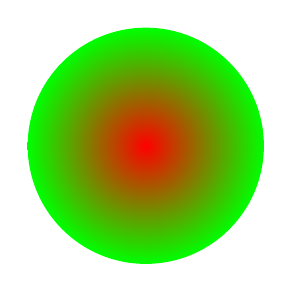
\begin{tikzpicture}
        \draw[draw=none,inner color=red, outer color=green] (0,0) circle (1.5cm);
      \end{tikzpicture}
         \end{tikzfigure}
			 \innerblock[]{Inner Blocks}{Inner blocks may be created inside of blocks with the command \bs\texttt{innerblock[{\it options}]\{{\it Heading}\}\{{\it Text}\}} }
            \coloredbox{Text may be highlighted using colored boxes created by \bs\texttt{coloredbox[{\it options}]\{{\it Text\}}}}          

     }
     \note[targetoffsetx=-.05\textwidth,targetoffsety=9.5cm,innersep=.4cm,angle=-45,connection]{Optional arguments for the format of the poster}
     \block{The title matter}{
         The title is made by the standard \texttt{\bs maketitle[{\it options}]} command where you can alter the \texttt{width}, the spacing between the title and top of the poster (\texttt{titletotopverticalspace}), the bottom of the title to the main content of the poster (\texttt{titletoblockverticalspace}) and the space between the title information and the logo (\texttt{titlegraphictotitleverticalspace}).

         If the default format of the title is not to your liking, you can define the placement of the different items via the \texttt{\bs settitle} command, described in the manual.
     }
     \block{Blocks}{
         Blocks are arranged in a grid, by default, with width by default \texttt{\bs textwdith}.  They are created by the command
         \begin{quote}
             \bs\texttt{block [{\it options}] \{{\it title}\}\{{\it contents}\}}
         \end{quote}
         The title may be left empty, resulting in no title area being created for the block (as seen in a later block to the right).  Further blocks will be placed below automatically, at a distance defined by \texttt{blockverticalspace}.

         If you want to change the position of the title matter or the contents in the block, you may by setting in the options
         \begin{quote}
             \texttt{titleoffsetx, titleoffsety, bodyoffsetx, bodyoffsety}
         \end{quote}
         which let you adjust the vertical or horizontal position of the two parts of the block, respectively.  You can also make, relative to the default width, the title and block body by setting
         \begin{quote}
             \texttt{titlewidthscale, bodywidthscale}
         \end{quote}
         The title's alignment can be set by \texttt{titleleft, titlecenter, titleright}, the body may be shifted vertically by setting \texttt{bodyverticalshift}, and the shape of the block can be altered by setting \texttt{roundedcorners, linewidth}. The inner margins of the title can by set by \texttt{titleinnersep,bodyinnersep}.
     }

     \note[targetoffsetx=24cm, targetoffsety=-9cm,rotate=1,angle=270,radius=8cm,width=.75\textwidth,innersep=.4cm]{
         You can place notes that are ``attached'' to the previous block using the command
         \begin{quote} \texttt{\bs note[{\it options}]\{{\it contents}\}}\end{quote}
         The note is placed by default slightly to the right of a ``target'' in the center of the previous block.  The note style may also allow for a connection between the note and the ``target''.  \\
         The target may be shifted from the default by setting the options  \texttt{targetoffsetx, targetoffsety}, rotated by an angle with \texttt{rotate}, and its width with \texttt{width}.  The placement of the note in relation with the target is given in polar coordinates with \texttt{ radius, angle}. Please observe that notes are always drawn {\bf over} the other objects. They do not affect the placement of blocks.
      }

     \column{.45}
         \block{Columns}{
              By default, blocks are arranged in a single column. If you want multiple columns for your poster, you may use the \texttt{columns} environment. For example,
             \begin{quote}
                 \texttt{\noindent \bs begin\{columns\}\\
                 \bs column\{.6\}\\
                 \bs block\{\dots\}\{\dots\}\\
                 \bs column\{.4\}\\
                 \bs block\{\dots\}\{\dots\}\\
                 \bs block\{\dots\}\{\dots\}\\
                 \bs end\{columns\}
                 }
             \end{quote}
             will create two columns of 60\% and 40\% the available width; spacing between successive columns is handled automatically.  The block command(s) following \texttt{\bs column} are the blocks to go in that column.  The number of columns is free to be chosen, but the relative widths must all be chosen.  If the widths sum to less than 1, empty space will be seen on the right.  If they sum to more than 1, the latter columns will be cut off.
         }

         \begin{subcolumns}
             \subcolumn{.45}
             \block{Subcolumns}{If you want to have an additional subdivision of columns inside a column, you may use the\\ \texttt{\bs subcolumns} environment inside of a column environment.  The functionality is similar to that of columns, but now the widths are relative to the width of the current column.}

             \subcolumn{.5}
             \block{}{An example use of subcolumns is.
                 \begin{quote}
                     \texttt{\bs begin\{subcolumns\}\\
                     \bs subcolumn\{.6\}\\
                     \bs block\{\dots\}\{\dots\}\\
                     \bs subcolumn\{.4\}\\
                     \bs block\{\dots\}\{\dots\}\\
                     \bs block\{\dots\}\{\dots\}\\
                     \bs end\{subcolumns\}
                     }
             \end{quote}
         }
         \end{subcolumns}

         \block[titlewidthscale=.8,bodywidthscale=.9,titleoffsety=9.5mm,bodyoffsety=9mm]{Changing the Poster's Appearance}{
             If the default appearance of the title, background, blocks, and notes is not desired, you may change the colors by calling the color style along with a general layout theme with the commands
             \begin{quote}
	       \texttt{\bs usecolorpalette}\{{\em color palette}\}\\
                 \texttt{\bs usecolorstyle\{{\em color style}\}}
             \end{quote}
             and
             \begin{quote}
                 \texttt{\bs usetheme\{{\em layout style}\}}
             \end{quote}
             where the color palette and style and layout style are either the name of a custom made or one of the offered predefined choices listed in the manual or the comments of this poster's source.  Individual changes can be made to the style of the  background, title matter, blocks, inner blocks, and notes by using one of the following (along with either a custom-designed style or a predefined style listed in the manual or the comments of this poster's source).  These changes are made with the commands
             \begin{quote}
                 \texttt{\bs usebackgroundstyle[]\{\}, \bs usetitlestyle[]\{\},\\ \bs useblockstyle[]\{\},\bs innerblockstyle[]\{\}, \bs usenotestyle[]\{\}}
             \end{quote}
             Custom styles for these can be made; this is detailed in the manual.
          }

     \end{columns}

     \block[titleoffsety=-1cm,bodyoffsety=-1cm]{Sample document}{\vspace{2em}
         This poster was created by the following commands (omitting the contents of the blocks and notes) to give a sense of how different objects are created and options used.
         \begin{quote}
             \texttt{\bs documentclass[25pt, a0paper, portrait, margin=0mm, innermargin=15mm,
         blockverticalspace=15mm, colspace=15mm, subcolspace=8mm]\{tikzposter\}\\
             \bs title\{Using tikzposter\} \bs author\{Pascal Richter, Elena Botoeva, Richard Barnard, \& Dirk Surmann\} \bs institute\{\}\\
              \bs usetheme\{Autumn\}\bs usecolorstyle[colorPalette=BrownBlueOrange]\{Germany\}\\
             \bs begin\{document\}\bs maketitle\\
             \bs begin\{columns\} \bs column\{0.55\}\\
             \bs block\{Creating the document\}\{The document\dots\} \bs note[targetoffsetx=-.05\bs textwidth,targetoffsety=9.5cm,innersep=.4cm,angle=-45,connection]\{\dots\}\\
             \bs block\{The title matter\}\{The title\dots\}\\
             \bs block\{Blocks\}\{Blocks are\dots\} \bs note[targetoffsetx=24cm, targetoffsety=-9cm,rotate=1,angle=270,radius=8cm,width=.75\bs textwidth,innersep=.4cm]\{You can\dots\}\\
             \bs column\{0.45\} \bs block\{Columns\}\{By default,\dots\}\\
             \bs begin\{subcolumns\} \bs subcolumn\{.45\}
             \bs block\{Subcolumns\}\{If you\dots\}
             \bs subcolumn\{.5\} \bs block\{\}\{An example\dots\} 
             \bs end\{subcolumns\}\\
             \bs block[titlewidthscale=.8,bodywidthscale=.9,titleoffsety=9.5mm,bodyoffsety=9mm]\{Changing the Poster's Appearance\}\{If the default\dots\}
             \bs end\{columns\}\\
             \bs block[titleoffsety=-1cm,bodyoffsety=-1cm]\{Sample document\}\{This poster\dots\}\\
             \bs end\{document\}
             }
         \end{quote}
     }

 \end{document}

%    \end{macrocode}
%    \begin{macrocode}
%</tikzposter-example.tex>
%    \end{macrocode}
%
% \section{Implementation}
% \subsection*{Color themes}
% \setcounter{CodelineNo}{0}
%    \begin{macrocode}
%<*tikzposterColorstyles.tex>
%    \end{macrocode} 
%    \begin{macrocode}
 
\definecolorstyle{Default}{
    % Define default colors
    % GrayBlueYellow
    \definecolor{colorOne}{HTML}{DDDDDD}
    \definecolor{colorTwo}{HTML}{0066A8}
    \definecolor{colorThree}{HTML}{FCE565}%FCF0AD}
}{
     % Background Colors
    \colorlet{backgroundcolor}{colorOne}
    \colorlet{framecolor}{colorTwo}
    % Title Colors
    \colorlet{titlefgcolor}{black}
    \colorlet{titlebgcolor}{white}
    % Block Colors
    \colorlet{blocktitlebgcolor}{colorTwo}
    \colorlet{blocktitlefgcolor}{white}
    \colorlet{blockbodybgcolor}{white}
    \colorlet{blockbodyfgcolor}{black}
    % Innerblock Colors
    \colorlet{innerblocktitlebgcolor}{colorThree}
    \colorlet{innerblocktitlefgcolor}{black}
    \colorlet{innerblockbodybgcolor}{white}
    \colorlet{innerblockbodyfgcolor}{black}
    % Note colors
    \colorlet{notefgcolor}{black}
    \colorlet{notebgcolor}{colorThree!70!white}
    \colorlet{notefrcolor}{colorThree}
 }

\definecolorstyle{Australia}{
    % Define default colors
    %GreenGrayViolet
    \definecolor{colorOne}{HTML}{A2E2C7}
    \definecolor{colorTwo}{HTML}{56555A}
    \definecolor{colorThree}{HTML}{C9AECF}
}{
     % Background Colors
    \colorlet{backgroundcolor}{colorOne}
    \colorlet{framecolor}{colorOne!50!colorTwo}
    % Title Colors
    \colorlet{titlefgcolor}{black}
    \colorlet{titlebgcolor}{white}
    % Block Colors
    \colorlet{blocktitlebgcolor}{colorTwo}
    \colorlet{blocktitlefgcolor}{white}
    \colorlet{blockbodybgcolor}{white}
    \colorlet{blockbodyfgcolor}{black}
    % Innerblock Colors
    \colorlet{innerblocktitlebgcolor}{colorThree}
    \colorlet{innerblocktitlefgcolor}{black}
    \colorlet{innerblockbodybgcolor}{white}
    \colorlet{innerblockbodyfgcolor}{black}
    % Note colors
    \colorlet{notefgcolor}{black}
    \colorlet{notebgcolor}{colorThree}
    \colorlet{notefrcolor}{colorThree}
 }

\definecolorstyle{Britain}{
    % Define default colors
    % BlueGrayOrange
    \definecolor{colorOne}{HTML}{116699}
    \definecolor{colorTwo}{HTML}{CCCCCC}
    \definecolor{colorThree}{HTML}{CC6633}
}{
     % Background Colors
    \colorlet{backgroundcolor}{colorOne}
    \colorlet{framecolor}{colorTwo}
    % Title Colors
    \colorlet{titlefgcolor}{black}
    \colorlet{titlebgcolor}{white}
    % Block Colors
    \colorlet{blocktitlebgcolor}{colorTwo}
    \colorlet{blocktitlefgcolor}{colorOne}
    \colorlet{blockbodybgcolor}{white}
    \colorlet{blockbodyfgcolor}{black}
    % Innerblock Colors
    \colorlet{innerblocktitlebgcolor}{colorThree}
    \colorlet{innerblocktitlefgcolor}{white}
    \colorlet{innerblockbodybgcolor}{white}
    \colorlet{innerblockbodyfgcolor}{black}
    % Note colors
    \colorlet{notefgcolor}{black}
    \colorlet{notebgcolor}{colorThree!40!white}
    \colorlet{notefrcolor}{colorThree!60!white}
 }

\definecolorstyle{Sweden}{
    % Define default colors
    % BlueGrayOrange
    \definecolor{colorOne}{HTML}{116699}
    \definecolor{colorTwo}{HTML}{CCCCCC}
    \definecolor{colorThree}{HTML}{CC6633}
}{
     % Background Colors
    \colorlet{backgroundcolor}{colorOne!40!white}
    \colorlet{framecolor}{colorTwo}
    % Title Colors
    \colorlet{titlefgcolor}{black}
    \colorlet{titlebgcolor}{white}
    % Block Colors
    \colorlet{blocktitlebgcolor}{colorTwo!70!black}
    \colorlet{blocktitlefgcolor}{colorOne}
    \colorlet{blockbodybgcolor}{white!90!colorTwo}
    \colorlet{blockbodyfgcolor}{black}
    % Innerblock Colors
    \colorlet{innerblocktitlebgcolor}{colorThree}
    \colorlet{innerblocktitlefgcolor}{white}
    \colorlet{innerblockbodybgcolor}{white}
    \colorlet{innerblockbodyfgcolor}{black}
    % Note colors
    \colorlet{notefgcolor}{black}
    \colorlet{notebgcolor}{colorThree!50!white}
    \colorlet{notefrcolor}{colorThree!50!white}
 }

\definecolorstyle{Spain}{
    % Define default colors
    % BlueGrayOrange
    \definecolor{colorOne}{HTML}{116699}
    \definecolor{colorTwo}{HTML}{CCCCCC}
    \definecolor{colorThree}{HTML}{CC6633}
}{
     % Background Colors
    \colorlet{backgroundcolor}{colorOne!55!white}
    \colorlet{framecolor}{colorTwo}
    % Title Colors
    \colorlet{titlefgcolor}{white}
    \colorlet{titlebgcolor}{colorOne}
    % Block Colors
    \colorlet{blocktitlebgcolor}{colorOne!80!black}
    \colorlet{blocktitlefgcolor}{white}
    \colorlet{blockbodybgcolor}{white}
    \colorlet{blockbodyfgcolor}{black}
    % Innerblock Colors
    \colorlet{innerblocktitlebgcolor}{colorThree}
    \colorlet{innerblocktitlefgcolor}{white}
    \colorlet{innerblockbodybgcolor}{white}
    \colorlet{innerblockbodyfgcolor}{black}
    % Note colors
    \colorlet{notefgcolor}{black}
    \colorlet{notebgcolor}{colorThree!50!white}
    \colorlet{notefrcolor}{colorThree}
 }

\definecolorstyle{Russia}{
    % Define default colors
    % BlueGrayOrange
    \definecolor{colorOne}{HTML}{116699}
    \definecolor{colorTwo}{HTML}{CCCCCC}
    \definecolor{colorThree}{HTML}{CC6633}
}{
     % Background Colors
    \colorlet{backgroundcolor}{white}
    \colorlet{framecolor}{colorOne!50!colorThree!30!}
    % Title Colors
    \colorlet{titlefgcolor}{white}
    \colorlet{titlebgcolor}{colorOne!70!black}
    % Block Colors
    \colorlet{blocktitlebgcolor}{colorThree!80!colorTwo!80!black}
    \colorlet{blocktitlefgcolor}{white}
    \colorlet{blockbodybgcolor}{colorTwo!40}
    \colorlet{blockbodyfgcolor}{black}
    % Innerblock Colors
    \colorlet{innerblocktitlebgcolor}{colorTwo!40}
    \colorlet{innerblocktitlefgcolor}{black}
    \colorlet{innerblockbodybgcolor}{colorTwo}
    \colorlet{innerblockbodyfgcolor}{black}
    % Note colors
    \colorlet{notefgcolor}{black}
    \colorlet{notebgcolor}{colorTwo}
    \colorlet{notefrcolor}{colorTwo}
 }

\definecolorstyle{Denmark}{
    % Define default colors
    % PurpleGrayBlue
    \definecolor{colorOne}{HTML}{AE0D45}
    \definecolor{colorTwo}{HTML}{7F8897}
    \definecolor{colorThree}{HTML}{C8512D}
}{
     % Background Colors
    \colorlet{backgroundcolor}{white}
    \colorlet{framecolor}{white}
    % Title Colors
    \colorlet{titlebgcolor}{colorOne}
    \colorlet{titlefgcolor}{white}
    % Block Colors
    \colorlet{blocktitlebgcolor}{colorTwo}
    \colorlet{blocktitlefgcolor}{colorOne}
    \colorlet{blockbodybgcolor}{white}
    \colorlet{blockbodyfgcolor}{black}
    % Innerblock Colors
    \colorlet{innerblocktitlebgcolor}{colorThree}
    \colorlet{innerblocktitlefgcolor}{white}
    \colorlet{innerblockbodybgcolor}{white}
    \colorlet{innerblockbodyfgcolor}{black}
    % Note colors
    \colorlet{notefgcolor}{black}
    \colorlet{notebgcolor}{colorTwo!50!white}
    \colorlet{notefrcolor}{colorTwo!50!white}
 }

\definecolorstyle{Germany}{
    % Define default colors
    % BrownOrangeBlue
    \definecolor{colorOne}{HTML}{8C7269}
    \definecolor{colorTwo}{HTML}{E89261}
    \definecolor{colorThree}{HTML}{A2C4D9}
}{
     % Background Colors
    \colorlet{backgroundcolor}{colorTwo}
    \colorlet{framecolor}{colorThree}
    % Title Colors
    \colorlet{titlebgcolor}{colorOne}
    \colorlet{titlefgcolor}{white}
    % Block Colors
    \colorlet{blocktitlebgcolor}{white}
    \colorlet{blocktitlefgcolor}{colorOne}
    \colorlet{blockbodybgcolor}{white}
    \colorlet{blockbodyfgcolor}{black}
    % Innerblock Colors
    \colorlet{innerblocktitlebgcolor}{white}
    \colorlet{innerblocktitlefgcolor}{black}
    \colorlet{innerblockbodybgcolor}{colorThree}
    \colorlet{innerblockbodyfgcolor}{black}
    % Note colors
    \colorlet{notefgcolor}{black}
    \colorlet{notebgcolor}{colorThree}
    \colorlet{notefrcolor}{colorThree}
 }



%    \end{macrocode}
%    \begin{macrocode}
%</tikzposterColorstyles.tex>
%    \end{macrocode}
%
%
% \subsection*{Initial code}
% \setcounter{CodelineNo}{0}
%    \begin{macrocode}
%<*tikzposter.cls>
%    \end{macrocode} 
%    \begin{macrocode}

\NeedsTeXFormat{LaTeX2e}
\ProvidesClass{tikzposter}[2014/01/15 v2.0 LaTeX document class for Posters]

 % --------------------------------------- %
 % Loading Packages
\usepackage{xkeyval}
\usepackage{calc}
\usepackage{ifthen}
\usepackage{ae}
\usepackage{xstring}
\usepackage{etoolbox}
\usepackage{tikz}
    \usetikzlibrary{shapes,decorations,shadows,backgrounds,calc,fadings,fit}
    \usetikzlibrary{decorations.pathmorphing}
    \usepgflibrary{arrows}

 % --------------------------------------- %
 % Paper parameter
\newif\ifTP@hugefontsize
\newdimen\TP@innermargin
\newdimen\TP@visibletextwidth
\newdimen\TP@visibletextheight

 % Title parameter
\newdimen\TP@titlewidth
\newdimen\titlewidth
\newdimen\TP@titlelinewidth
\newdimen\titlelinewidth
\def\titleroundedcorners{}
\newdimen\titleinnersep
\newdimen\TP@titleinnersep
\newdimen\TP@titletotopverticalspace
\newdimen\titletotopverticalspace
\newdimen\TP@titletoblockverticalspace
\newdimen\TP@titleheight
\newdimen\titleheight
\newdimen\titlegraphicheight
\newdimen\titleposleft
\newdimen\titleposright
\newdimen\titlepostop
\newdimen\titleposbottom
\newdimen\TP@titlegraphictotitledistance
\def\TP@titletextscale{1}

 % Maketitle parameter
\def\@title{~}
\def\title#1{\gdef\@title{\scalebox{\TP@titletextscale}{#1}}}
\def\@author{~}
\def\@institute{~}
\def\@titlegraphic{~}

 % Affection parameter
\newif\ifTP@showlatexaffection

 % Column parameter
\newif\ifTP@columnEnvironment
\TP@columnEnvironmentfalse
\newif\ifTP@subcolumnEnvironment
\TP@subcolumnEnvironmentfalse
\newdimen\TP@colspace
\newdimen\TP@coltop
\newdimen\TP@colbottom
\newdimen\TP@colcenter
\newdimen\colwidth

 % Subcolumn parameter
\newdimen\TP@subcolspace
\newdimen\TP@subcoltop
\newdimen\TP@subcolbottom
\newdimen\TP@subcolcenter
\newdimen\subcolwidth

 % Block parameter
\newdimen\TP@blockverticalspace
\newdimen\TP@blockcenter
\newdimen\TP@blocktitleinnersep
\newdimen\blocktitleinnersep
\newdimen\TP@blockbodyinnersep
\newdimen\blockbodyinnersep
\newbox\TP@blocktitlebox
\newbox\TP@blockbodybox
\def\TP@blocktitleAlignment{}
\newif\ifBlockHasTitle
\newdimen\TP@blocktitlewidth
\newdimen\TP@blockbodywidth
\newdimen\TP@blockbodyheight
\newdimen\TP@blocktitleheight
\newdimen\TP@blocktop
\newdimen\TP@blocktitleoffsetx
\newdimen\TP@blocktitleoffsety
\newdimen\TP@blockbodyoffsetx
\newdimen\TP@blockbodyoffsety
\newdimen\TP@blockbodyverticalshift
\def\blockroundedcorners{}
\newdimen\blocklinewidth

 % Innerblock parameter
\newdimen\TP@innerblockcenter
\newdimen\TP@innerblocktitleinnersep
\newdimen\innerblocktitleinnersep
\newdimen\TP@innerblockbodyinnersep
\newdimen\innerblockbodyinnersep
\newbox\TP@innerblocktitlebox
\newbox\TP@innerblockbodybox
\def\TP@innerblocktitleAlignment{}
\newif\ifInnerblockHasTitle
\newdimen\TP@innerblocktitlewidth  
\newdimen\TP@innerblockbodywidth
\newdimen\TP@innerblockbodyheight
\newdimen\TP@innerblocktitleheight
\newdimen\TP@innerblocktitleoffsetx
\newdimen\TP@innerblocktitleoffsety
\newdimen\TP@innerblockbodyoffsetx
\newdimen\TP@innerblockbodyoffsety
\newdimen\TP@innerblockbodyverticalshift
\def\innerblockroundedcorners{}
\newdimen\innerblocklinewidth

 % Coloredbox parameter
\newbox\TP@coloredbox
\newdimen\TP@coloredboxwidth
\def\TP@coloredboxroundedcorners{}
\newdimen\TP@coloredboxlinewidth
\newdimen\TP@coloredboxinnersep
\newdimen\TP@coloredboxheight

 % Note parameter
\newdimen\TP@noteinnersep
\newdimen\noteinnersep
\newdimen\TP@notetargetoffsetx
\newdimen\TP@notetargetoffsety
\def\TP@noteangle{}
\newdimen\TP@noteradius
\newdimen\TP@notewidth
\newdimen\TP@noteheight
\newif\ifNoteHasConnection
\newbox\TP@notebox
\def\noterotate{}
\def\noteroundedcorners{}
\newdimen\notelinewidth

 % --------------------------------------- %
 % Declaring options
\DeclareOptionX{12pt}{\TP@hugefontsizefalse \PassOptionsToClass{\CurrentOption}{extarticle}}
\DeclareOptionX{14pt}{\TP@hugefontsizefalse \PassOptionsToClass{\CurrentOption}{extarticle}}
\DeclareOptionX{17pt}{\TP@hugefontsizefalse \PassOptionsToClass{\CurrentOption}{extarticle}}
\DeclareOptionX{20pt}{\TP@hugefontsizefalse \PassOptionsToClass{\CurrentOption}{extarticle}}
\DeclareOptionX{25pt}{\TP@hugefontsizetrue}
\DeclareOptionX{fleqn}{\PassOptionsToClass{\CurrentOption}{extarticle}}
\DeclareOptionX{leqno} {\PassOptionsToClass{\CurrentOption}{extarticle}}
\DeclareOptionX{a0paper}{\PassOptionsToPackage{\CurrentOption}{geometry}}
\DeclareOptionX{a1paper}{\PassOptionsToPackage{\CurrentOption}{geometry}}
\DeclareOptionX{a2paper}{\PassOptionsToPackage{\CurrentOption}{geometry}}
\DeclareOptionX{landscape}{\PassOptionsToPackage{\CurrentOption}{geometry}}
\DeclareOptionX{portrait}{\PassOptionsToPackage{\CurrentOption}{geometry}}
\DeclareOptionX{margin}[20mm]{\PassOptionsToPackage{margin=#1}{geometry}}
\DeclareOptionX{innermargin}{\TP@innermargin=#1}
\DeclareOptionX{colspace}{\TP@colspace=#1}
\DeclareOptionX{subcolspace}{\TP@subcolspace=#1}
\DeclareOptionX{blockverticalspace}{\TP@blockverticalspace=#1}
\DeclareOptionX*{{\PackageWarning{tikzposter}{Unknown Option \CurrentOption.}}}

 % Executing options
\ExecuteOptionsX{
    25pt,
    a0paper,
    portrait,
    margin=0mm,
    innermargin=15mm,
    colspace=15mm,
    subcolspace=8mm,
    blockverticalspace=15mm
}
\ProcessOptionsX \relax
\LoadClass{extarticle}
\RequirePackage{geometry}
\ifTP@hugefontsize
    \input{a0size.sty}
    \renewcommand{\tiny}{\fontsize{12}{14}\selectfont}
    \renewcommand{\scriptsize}{\fontsize{14.4}{18}\selectfont}
    \renewcommand{\footnotesize}{\fontsize{17.28}{22}\selectfont}
    \renewcommand{\small}{\fontsize{20.74}{25}\selectfont}
    \renewcommand{\normalsize}{\fontsize{24.88}{30}\selectfont}
    \renewcommand{\large}{\fontsize{29.86}{37}\selectfont}
    \renewcommand{\Large}{\fontsize{35.83}{45}\selectfont}
    \renewcommand{\LARGE}{\fontsize{43}{54}\selectfont}
    \renewcommand{\huge}{\fontsize{51.6}{64}\selectfont}
    \renewcommand{\Huge}{\fontsize{61.92}{77}\selectfont}
\fi
\normalsize
\pagestyle{empty}
\setlength{\TP@visibletextwidth}{\textwidth-2\TP@innermargin}
\setlength{\TP@visibletextheight}{\textheight-2\TP@innermargin}
\pgfdeclarelayer{backgroundlayer}
\pgfdeclarelayer{notelayer}
\pgfsetlayers{backgroundlayer,main,notelayer}

 % --------------------------------------- %
 % Background styles
\gdef\definebackgroundstyle#1#2{\expandafter\gdef\csname TP@backgroundstyle#1\endcsname{#2}}

\gdef\usebackgroundstyle#1{
    \ifcsname TP@backgroundstyle#1\endcsname
         \gdef\TP@backgroundstyle{\csname TP@backgroundstyle#1\endcsname} % save macro
    \else
        \PackageWarning{tikzposter}{Unknown backgroundstyle `#1'.}
    \fi
}

 % --------------------------------------- %
 % Title styles
\gdef\definetitlestyle#1#2#3{
    \expandafter\gdef\csname TP@titlestyle#1Defaultvalues\endcsname{\gpresetkeys{title}{#2}{}}
    \expandafter\gdef\csname TP@titlestyle#1\endcsname{#3}
}

\define@key{title}{width}{\TP@titlewidth=#1 \titlewidth=#1}
\define@key{title}{roundedcorners}{\gdef\titleroundedcorners{#1}}
\define@key{title}{linewidth}{\TP@titlelinewidth=#1 \titlelinewidth=#1}
\define@key{title}{innersep}{\TP@titleinnersep=#1 \titleinnersep=#1}
\define@key{title}{titletotopverticalspace}{\TP@titletotopverticalspace=#1 \titletotopverticalspace=#1}
\define@key{title}{titletoblockverticalspace}{\TP@titletoblockverticalspace=#1}
\define@key{title}{titlegraphictotitledistance}{\TP@titlegraphictotitledistance=#1}
\define@key{title}{titletextscale}{\TP@titletextscale=#1}
\newcommand\usetitlestyle[2][]{
    \ifcsname TP@titlestyle#2\endcsname
         \csname TP@titlestyle#2Defaultvalues\endcsname\gpresetkeys{title}{#1}{} % call macro
         \gdef\TP@titlestyle{\csname TP@titlestyle#2\endcsname} % save macro
    \else
        \PackageWarning{tikzposter}{Unknown titlestyle `#2'.}
    \fi
}

 % --------------------------------------- %
 % Title
\gdef\TP@maketitle{
    \centering
    \vbox{
    \@titlegraphic
        \\[\TP@titlegraphictotitledistance]
        \centering
        \color{titlefgcolor}
        {\bfseries \Huge \sc \@title \par}
        \vspace*{1em}
        {\huge \@author \par}
        \vspace*{1em}
        {\LARGE \@institute}
    }
}

\gdef\institute#1{\gdef\@institute{#1}}
\gdef\titlegraphic#1{\gdef\@titlegraphic{#1}}

\newenvironment{settitle}{
    \makeatletter
    \renewcommand{\TP@maketitle}
}{
    \makeatother
}


\renewcommand\maketitle[1][]{  % #1 keys
    \normalsize
    \setkeys{title}{#1}
    % Title dummy to get title height
    \node[transparent,inner sep=\TP@titleinnersep, line width=\TP@titlelinewidth, anchor=north, minimum width=\TP@visibletextwidth-2\TP@titleinnersep]
        (TP@title) at ($(0, 0.5\textheight-\TP@titletotopverticalspace)$) {\parbox{\TP@titlewidth-2\TP@titleinnersep}{\TP@maketitle}};
    \draw let \p1 = ($(TP@title.north)-(TP@title.south)$) in node {
        \setlength{\TP@titleheight}{\y1}
        \setlength{\titleheight}{\y1}
        \global\TP@titleheight=\TP@titleheight
        \global\titleheight=\titleheight
    };

    % Compute title position
    \setlength{\titleposleft}{-0.5\titlewidth}
    \setlength{\titleposright}{\titleposleft+\titlewidth}
    \setlength{\titlepostop}{0.5\textheight-\TP@titletotopverticalspace}
    \setlength{\titleposbottom}{\titlepostop-\titleheight}

    % Title style (background)
    \TP@titlestyle

    % Title node
    \node[inner sep=\TP@titleinnersep, line width=\TP@titlelinewidth, anchor=north, minimum width=\TP@visibletextwidth-2\TP@titleinnersep]
        at (0,0.5\textheight-\TP@titletotopverticalspace) {\parbox{\TP@titlewidth-2\TP@titleinnersep}{\TP@maketitle}};

    % Settings for blocks
    \normalsize
    \setlength{\TP@blocktop}{\titleposbottom-\TP@titletoblockverticalspace}
}

 % --------------------------------------- %
 % Block styles
\gdef\defineblockstyle#1#2#3{
    \expandafter\gdef\csname TP@blockstyle#1Defaultvalues\endcsname{\gpresetkeys{block}{#2}{}}
    \expandafter\gdef\csname TP@blockstyle#1\endcsname{#3}
}

\define@key{block}{titlewidthscale}{\setlength{\TP@blocktitlewidth}{#1\TP@blocktitlewidth}}
\define@key{block}{bodywidthscale}{\setlength{\TP@blockbodywidth}{#1\TP@blockbodywidth}}
\define@boolkey{block}{titleleft}[true]{\ifKV@block@titleleft \gdef\TP@blocktitleAlignment{\raggedright} \fi}
\define@boolkey{block}{titlecenter}[true]{\ifKV@block@titlecenter \gdef\TP@blocktitleAlignment{\centering} \fi}
\define@boolkey{block}{titleright}[true]{\ifKV@block@titleright \gdef\TP@blocktitleAlignment{\raggedleft} \fi}
\define@key{block}{titleoffsetx}{\TP@blocktitleoffsetx=#1}
\define@key{block}{titleoffsety}{\TP@blocktitleoffsety=#1}
\define@key{block}{bodyoffsetx}{\TP@blockbodyoffsetx=#1}
\define@key{block}{bodyoffsety}{\TP@blockbodyoffsety=#1}
\define@key{block}{bodyverticalshift}{\TP@blockbodyverticalshift=#1}
\define@key{block}{roundedcorners}{\gdef\blockroundedcorners{#1}}
\define@key{block}{linewidth}{\blocklinewidth=#1}
\define@key{block}{titleinnersep}{\TP@blocktitleinnersep=#1 \blocktitleinnersep=#1}
\define@key{block}{bodyinnersep}{\TP@blockbodyinnersep=#1 \blockbodyinnersep=#1}

\newcommand\useblockstyle[2][]{
    \ifcsname TP@blockstyle#2\endcsname
        \csname TP@blockstyle#2Defaultvalues\endcsname\gpresetkeys{block}{#1}{} % call macro
        \gdef\TP@blockstyle{\csname TP@blockstyle#2\endcsname} % save macro
    \else
        \PackageWarning{tikzposter}{Unknown blockstyle `#2'.}
    \fi
}

 % --------------------------------------- %
 % Block
\newcommand\block[3][]{  % #1 keys   #2 title   #3 text
    % Block position
    \normalsize
    \ifTP@subcolumnEnvironment
        \TP@blocktitlewidth=\subcolwidth
        \TP@blockbodywidth=\subcolwidth
        \TP@blockcenter=\TP@subcolcenter
    \else
        \ifTP@columnEnvironment
            \TP@blocktitlewidth=\colwidth
            \TP@blockbodywidth=\colwidth
            \TP@blockcenter=\TP@colcenter
        \else
            \setlength\TP@blocktitlewidth{\TP@visibletextwidth}
            \setlength\TP@blockbodywidth{\TP@visibletextwidth}
            \TP@blockcenter=0pt
        \fi
    \fi
    
    % Set parameter
    \setkeys{block}{#1}
    
    % Settings for Subcolumns
    \ifTP@subcolumnEnvironment \else \ifTP@columnEnvironment \else
        \setlength\TP@blocktitlewidth{\TP@blocktitlewidth-\blocklinewidth}
        \setlength\TP@blockbodywidth{\TP@blockbodywidth-\blocklinewidth}
        \TP@blockcenter=0pt
    \fi \fi
    
    % Get height of title
    \ifstrempty{#2}{
        \BlockHasTitlefalse
        \setlength{\TP@blocktitleheight}{0pt}
    }{
        \BlockHasTitletrue
        \setbox\TP@blocktitlebox=\hbox{%
            \pgfinterruptpicture%
            \parbox{\TP@blocktitlewidth-2\TP@blocktitleinnersep}{%
                \bf\LARGE\color{blocktitlefgcolor}\TP@blocktitleAlignment#2\par\normalsize}%
            \endpgfinterruptpicture%
        }%
        \setlength{\TP@blocktitleheight}{\ht\TP@blocktitlebox + \dp\TP@blocktitlebox +2\TP@blocktitleinnersep}
    }
    
    % Get height of body
    \setbox\TP@blockbodybox=\hbox{
        \pgfinterruptpicture%
        \parbox{\TP@blockbodywidth-2\TP@blockbodyinnersep-\TP@blockbodyoffsetx}{%
            \vspace*{\TP@blockbodyverticalshift}\large\color{blockbodyfgcolor}#3\par\normalsize}%
        \endpgfinterruptpicture%
    }%
    \setlength{\TP@blockbodyheight}{\ht\TP@blockbodybox + \dp\TP@blockbodybox +2\TP@blockbodyinnersep}
    
    % Set coordinates
    \node[minimum width=\TP@blocktitlewidth, minimum height=\TP@blocktitleheight, anchor=center] (blocktitle)%
        at (\TP@blockcenter+\TP@blocktitleoffsetx, {\TP@blocktop-0.5\TP@blocktitleheight+\TP@blocktitleoffsety}){};
    \ifBlockHasTitle
        \node[minimum width=\TP@blockbodywidth, minimum height=\TP@blockbodyheight, anchor=center] (blockbody)%
            at (\TP@blockcenter+\TP@blockbodyoffsetx, {\TP@blocktop-\TP@blocktitleheight-0.5\TP@blockbodyheight+\TP@blockbodyoffsety}){};
    \else
        \node[minimum width=\TP@blockbodywidth, minimum height=\TP@blockbodyheight, anchor=center] (blockbody)%
            at (\TP@blockcenter+\TP@blockbodyoffsetx, {\TP@blocktop-\TP@blocktitleheight-0.5\TP@blockbodyheight}){};
    \fi
    
    % Draw style
    \TP@blockstyle
    
    % Draw text
    \ifBlockHasTitle
        \node[text width=\TP@blocktitlewidth-2\TP@blocktitleinnersep, inner sep=\TP@blocktitleinnersep, anchor=center]%
            at (blocktitle){\box\TP@blocktitlebox};
    \fi
    \node[text width=\TP@blockbodywidth-2\TP@blockbodyinnersep, inner sep=\TP@blockbodyinnersep, anchor=center]%
        at (blockbody){\box\TP@blockbodybox};
    
    % Set position parameter
    \draw let \p1 = (blockbody.south) in node {
        \setlength{\TP@blocktop}{\y1-\TP@blockverticalspace}
        \global\TP@blocktop=\TP@blocktop
    };
    \ifTP@subcolumnEnvironment
        \setlength{\TP@subcolbottom}{\minof{\TP@subcolbottom}{\TP@blocktop}}
        \global\TP@subcolbottom=\TP@subcolbottom
    \else
        \ifTP@columnEnvironment
            \setlength{\TP@colbottom}{\minof{\TP@colbottom}{\TP@blocktop}}
            \global\TP@colbottom=\TP@colbottom
        \fi
    \fi
}

 % --------------------------------------- %
 % Innerblock styles
\gdef\defineinnerblockstyle#1#2#3{
    \expandafter\gdef\csname TP@innerblockstyle#1Defaultvalues\endcsname{\gpresetkeys{innerblock}{#2}{}}
    \expandafter\gdef\csname TP@innerblockstyle#1\endcsname{#3}
}

\define@key{innerblock}{titlewidth}{\setlength{\TP@innerblocktitlewidth}{#1}}
\define@key{innerblock}{bodywidth}{\setlength{\TP@innerblockbodywidth}{#1}}
\define@key{innerblock}{titlewidthscale}{\setlength{\TP@innerblocktitlewidth}{#1\TP@innerblocktitlewidth}}
\define@key{innerblock}{bodywidthscale}{\setlength{\TP@innerblockbodywidth}{#1\TP@innerblockbodywidth}}
\define@boolkey{innerblock}{titleleft}[true]{\ifKV@innerblock@titleleft \gdef\TP@innerblocktitleAlignment{\raggedright} \fi}
\define@boolkey{innerblock}{titlecenter}[true]{\ifKV@innerblock@titlecenter \gdef\TP@innerblocktitleAlignment{\centering} \fi}
\define@boolkey{innerblock}{titleright}[true]{\ifKV@innerblock@titleright \gdef\TP@innerblocktitleAlignment{\raggedleft} \fi}
\define@key{innerblock}{titleoffsetx}{\TP@innerblocktitleoffsetx=#1}
\define@key{innerblock}{titleoffsety}{\TP@innerblocktitleoffsety=#1}
\define@key{innerblock}{bodyoffsetx}{\TP@innerblockbodyoffsetx=#1}
\define@key{innerblock}{bodyoffsety}{\TP@innerblockbodyoffsety=#1}
\define@key{innerblock}{bodyverticalshift}{\TP@innerblockbodyverticalshift=#1}
\define@key{innerblock}{roundedcorners}{\gdef\innerblockroundedcorners{#1}}
\define@key{innerblock}{linewidth}{\innerblocklinewidth=#1}
\define@key{innerblock}{titleinnersep}{\TP@innerblocktitleinnersep=#1 \innerblocktitleinnersep=#1}
\define@key{innerblock}{bodyinnersep}{\TP@innerblockbodyinnersep=#1 \innerblockbodyinnersep=#1}
\define@key{innerblock}{titlebgcolor}{\definecolor{innerblocktitlebgcolor}{named}{#1}}
\define@key{innerblock}{titlefgcolor}{\definecolor{innerblocktitlefgcolor}{named}{#1}}
\define@key{innerblock}{bodybgcolor}{\definecolor{innerblockbodybgcolor}{named}{#1}}
\define@key{innerblock}{bodyfgcolor}{\definecolor{innerblockbodyfgcolor}{named}{#1}}

\newcommand\useinnerblockstyle[2][]{
    \ifcsname TP@innerblockstyle#2\endcsname
        \csname TP@innerblockstyle#2Defaultvalues\endcsname\gpresetkeys{innerblock}{#1}{} % call macro
        \gdef\TP@innerblockstyle{\csname TP@innerblockstyle#2\endcsname} % save macro
    \else
        \PackageWarning{tikzposter}{Unknown innerblockstyle `#2'.}
    \fi
}

 % --------------------------------------- %
 % Innerblock
\newcommand\innerblock[3][]{  % #1 keys   #2 title   #3 text
    % Settings for Innerblock
    \definecolor{innerblocktitlebgcolorTemp}{named}{innerblocktitlebgcolor}
    \definecolor{innerblocktitlefgcolorTemp}{named}{innerblocktitlefgcolor}
    \definecolor{innerblockbodybgcolorTemp}{named}{innerblockbodybgcolor}
    \definecolor{innerblockbodyfgcolorTemp}{named}{innerblockbodyfgcolor}
    \setlength{\TP@innerblocktitlewidth}{\linewidth}
    \setlength{\TP@innerblockbodywidth}{\linewidth}
    \setkeys{innerblock}{#1}
    
    \begin{tikzpicture}
        
        % Get center in x-direction
        \pgfmathsetlength{\TP@innerblockcenter}{max(\TP@innerblocktitlewidth,\TP@innerblockbodywidth)/2}
        
        % Get height of title
        \ifstrempty{#2}{
            \InnerblockHasTitlefalse
            \setlength{\TP@innerblocktitleheight}{0pt}
        }{
            \InnerblockHasTitletrue
            \setbox\TP@innerblocktitlebox=\hbox{%
                \pgfinterruptpicture%
                \parbox{\TP@innerblocktitlewidth-2\TP@innerblocktitleinnersep}{%
                    \bf\color{innerblocktitlefgcolor}\TP@innerblocktitleAlignment#2\par\normalsize}%
                \endpgfinterruptpicture%
                }
            \setlength{\TP@innerblocktitleheight}{\ht\TP@innerblocktitlebox + \dp\TP@innerblocktitlebox +2\TP@innerblocktitleinnersep}
        }
        
        % Get height of body
        \setbox\TP@innerblockbodybox=\hbox{
            \pgfinterruptpicture%
            \parbox{\TP@innerblockbodywidth-2\TP@innerblockbodyinnersep-\TP@innerblockbodyoffsetx}{%
                \vspace*{\TP@innerblockbodyverticalshift}%
                \color{innerblockbodyfgcolor}#3\par\normalsize}%
            \endpgfinterruptpicture%
        }%
        \setlength{\TP@innerblockbodyheight}{\ht\TP@innerblockbodybox + \dp\TP@innerblockbodybox +2\TP@innerblockbodyinnersep}
 
        % Set coordinates
        \node[minimum width=\TP@innerblocktitlewidth, minimum height=\TP@innerblocktitleheight, anchor=center] (innerblocktitle)
            at (\TP@innerblockcenter+\TP@innerblocktitleoffsetx, {-0.5\TP@innerblocktitleheight+\TP@innerblocktitleoffsety}) {};%
        \ifInnerblockHasTitle
            \node[minimum width=\TP@innerblockbodywidth, minimum height=\TP@innerblockbodyheight, anchor=center] (innerblockbody)
                at (\TP@innerblockcenter+\TP@innerblockbodyoffsetx, {-\TP@innerblocktitleheight-0.5\TP@innerblockbodyheight+\TP@innerblockbodyoffsety}) {};%    
        \else
           \node[minimum width=\TP@innerblockbodywidth, minimum height=\TP@innerblockbodyheight, anchor=center] (innerblockbody)
                at (\TP@innerblockcenter+\TP@innerblockbodyoffsetx, {-\TP@innerblocktitleheight-0.5\TP@innerblockbodyheight}) {};%    
        \fi
        
        % Draw style
        \TP@innerblockstyle
        
        % Draw text
        \ifInnerblockHasTitle
            \node[text width=\TP@innerblocktitlewidth-2\TP@innerblocktitleinnersep, inner sep=\TP@innerblocktitleinnersep, anchor= center]
                at (innerblocktitle) {\box\TP@innerblocktitlebox};%
        \fi
        \node[text width=\TP@innerblockbodywidth-2\TP@innerblockbodyinnersep, inner sep=\TP@innerblockbodyinnersep, anchor= center]
            at (innerblockbody) {\box\TP@innerblockbodybox};%
    \end{tikzpicture}
    
    % Reset colors
    \definecolor{innerblocktitlebgcolor}{named}{innerblocktitlebgcolorTemp}
    \definecolor{innerblocktitlefgcolor}{named}{innerblocktitlefgcolorTemp}
    \definecolor{innerblockbodybgcolor}{named}{innerblockbodybgcolorTemp}
    \definecolor{innerblockbodyfgcolor}{named}{innerblockbodyfgcolorTemp}
}

 % --------------------------------------- %
 % Coloredbox
\define@key{coloredbox}{width}{\setlength{\TP@coloredboxwidth}{#1}}
\define@key{coloredbox}{roundedcorners}{\gdef\TP@coloredboxroundedcorners{#1}}
\define@key{coloredbox}{linewidth}{\TP@coloredboxlinewidth=#1}
\define@key{coloredbox}{innersep}{\TP@coloredboxinnersep=#1}
\define@key{coloredbox}{bgcolor}{\definecolor{coloredboxbgcolorTemp}{named}{#1}}
\define@key{coloredbox}{fgcolor}{\definecolor{coloredboxfgcolorTemp}{named}{#1}}
\define@key{coloredbox}{framecolor}{\definecolor{coloredboxframecolorTemp}{named}{#1}}

\newcommand\coloredbox[2][]{  % #1 keys   #2 text
    % Settings for coloredbox
    \setlength{\TP@coloredboxwidth}{\TP@blocktitlewidth-4\TP@blocktitleinnersep}
    \setkeys{coloredbox}{%
    	width={\linewidth}, roundedcorners=15, linewidth=3.5pt, innersep=10pt,
	bgcolor=notebgcolor, fgcolor=notefgcolor, framecolor=notebgcolor, #1}
    
    \begin{tikzpicture}
        % Get height of text
        \setbox\TP@coloredbox=\hbox{
            \pgfinterruptpicture%
            \parbox{\TP@coloredboxwidth-2\TP@coloredboxinnersep}{%
                \color{coloredboxfgcolorTemp}#2\par\normalsize}%
            \endpgfinterruptpicture%
        }%
        \setlength{\TP@coloredboxheight}{\ht\TP@coloredbox + \dp\TP@coloredbox +2\TP@coloredboxinnersep}
        
        % Set coordinates
        \node[minimum width=\TP@coloredboxwidth, minimum height=\TP@coloredboxheight, anchor=center] (coloredbox)
            at (0.5\TP@coloredboxwidth, -0.5\TP@coloredboxheight) {};%
        
        % Draw style
        \begin{scope}[line width=\TP@coloredboxlinewidth, rounded corners=\TP@coloredboxroundedcorners]
            \draw[color=coloredboxframecolorTemp, fill=coloredboxbgcolorTemp] (coloredbox.south west) rectangle (coloredbox.north east);
        \end{scope}
        
        % Draw text
        \node[text width=\TP@coloredboxwidth-2\TP@coloredboxinnersep, inner sep=\TP@coloredboxinnersep, anchor= center]
            at (coloredbox) {\box\TP@coloredbox};%
    \end{tikzpicture}
   
    % Reset colors
    \definecolor{coloredboxbgcolor}{named}{coloredboxbgcolorTemp}
    \definecolor{coloredboxfgcolor}{named}{coloredboxfgcolorTemp}
}


 % --------------------------------------- %
 % Note styles
\gdef\definenotestyle#1#2#3{
    \expandafter\gdef\csname TP@notestyle#1Defaultvalues\endcsname{\gpresetkeys{note}{#2}{}}
    \expandafter\gdef\csname TP@notestyle#1\endcsname{#3}
}

\define@key{note}{targetoffsetx}{\TP@notetargetoffsetx=#1}
\define@key{note}{targetoffsety}{\TP@notetargetoffsety=#1}
\define@key{note}{angle}{\def\TP@noteangle{#1}}
\define@key{note}{radius}{\TP@noteradius=#1}
\define@key{note}{width}{\TP@notewidth=#1}
\define@boolkey{note}{connection}[true]{\NoteHasConnectiontrue \ifKV@note@connection \NoteHasConnectiontrue \else \NoteHasConnectionfalse \fi}
\define@key{note}{rotate}{\gdef\noterotate{#1}}
\define@key{note}{roundedcorners}{\gdef\noteroundedcorners{#1}}
\define@key{note}{linewidth}{\notelinewidth=#1}
\define@key{note}{innersep}{\TP@noteinnersep=#1 \noteinnersep=#1}
\newcommand\usenotestyle[2][]{
    \ifcsname TP@notestyle#2\endcsname
        \csname TP@notestyle#2Defaultvalues\endcsname\gpresetkeys{note}{#1}{} % call macro
        \gdef\TP@notestyle{\csname TP@notestyle#2\endcsname} % save macro
    \else
        \PackageWarning{tikzposter}{Unknown notestyle `#2'.}
    \fi
}

 % --------------------------------------- %
 % Note
\newcommand\note[2][]{  % #1 keys   #2 text
    \normalsize
    \setkeys{note}{#1}

    % Note box
    \setbox\TP@notebox=\hbox{%
        \pgfinterruptpicture%
        \parbox{\TP@notewidth-2\TP@noteinnersep}{\color{notefgcolor}#2\par\normalsize}%
        \endpgfinterruptpicture%
    }%
    \setlength{\TP@noteheight}{\ht\TP@notebox + \dp\TP@notebox +2\TP@noteinnersep}
    \pgfmathsetlength{\TP@noteheight}{max(\TP@noteheight,80pt)}
    
    % Set note coordinates
    \node (notetarget) at ($(blockbody)+(\TP@notetargetoffsetx,\TP@notetargetoffsety)$){};
    \node[minimum width=\TP@notewidth, minimum height=\TP@noteheight, anchor=center,rotate=\noterotate] (notecenter)
        at ($(notetarget)+({\TP@noteradius*cos(\TP@noteangle)},{\TP@noteradius*sin(\TP@noteangle)})$){};%
    
    % Draw note
    \begin{pgfonlayer}{notelayer}
        \TP@notestyle
        % Draw note text
        \node[text width=\TP@notewidth-2\TP@noteinnersep, inner sep=\TP@noteinnersep, anchor=center,rotate=\noterotate]%
            at (notecenter){\box\TP@notebox};
    \end{pgfonlayer}
}

 % --------------------------------------- %
 % Color palette
\gdef\definecolorpalette#1#2{\expandafter\gdef\csname TP@colorpalette#1\endcsname{#2}}

\gdef\usecolorpalette#1{
    \ifcsname TP@colorpalette#1\endcsname
         \csname TP@colorpalette#1\endcsname % call macro
    \else
        \PackageWarning{tikzposter}{Unknown color palette `#1'.}
    \fi
}

 % --------------------------------------- %
 % Color style
\gdef\definecolorstyle#1#2#3{
    \expandafter\gdef\csname TP@colorstyle#1Defaultvalues\endcsname{#2}
    \expandafter\gdef\csname TP@colorstyle#1\endcsname{#3}
}

\define@key{colors}{colorOne}{\colorlet{colorOne}{#1}}
\define@key{colors}{colorTwo}{\colorlet{colorTwo}{#1}}
\define@key{colors}{colorThree}{\colorlet{colorThree}{#1}}
\define@key{colors}{colorPalette}{\usecolorpalette{#1}}

\newcommand\usecolorstyle[2][]{  % #1 keys   #2 macroname
    \ifcsname TP@colorstyle#2\endcsname
         \csname TP@colorstyle#2Defaultvalues\endcsname % call macro
         \setkeys{colors}{#1} % set keys
         \csname TP@colorstyle#2\endcsname % call macro
    \else
        \PackageWarning{tikzposter}{Unknown color style `#2'.}
    \fi
}

 % --------------------------------------- %
 % Layouttheme
\gdef\definelayouttheme#1#2{\expandafter\gdef\csname TP@layouttheme#1\endcsname{#2}}

\gdef\usetheme#1{
    % Layout theme
    \ifcsname TP@layouttheme#1\endcsname
         \csname TP@layouttheme#1\endcsname % call macro
    \else
        \PackageWarning{tikzposter}{Unknown layouttheme `#1'.}
    \fi
}

 % Input Style and Theme Files
%%
%% This is file `tikzposterColorpalettes.tex',
%% generated with the docstrip utility.
%%
%% The original source files were:
%%
%% tikzposter.dtx  (with options: `tikzposterColorpalettes.tex')
%% 
%% This is a generated file.
%% 
%% Copyright (C) 2014 by Pascal Richter, Elena Botoeva, Richard Barnard, and Dirk Surmann
%% 
%% This file may be distributed and/or modified under the
%% conditions of the LaTeX Project Public License, either
%% version 2.0 of this license or (at your option) any later
%% version. The latest version of this license is in:
%% 
%% http://www.latex-project.org/lppl.txt
%% 
%% and version 2.0 or later is part of all distributions of
%% LaTeX version 2013/12/01 or later.
%% 










\definecolorpalette{Default}{
    % GrayBlueYellow
    \definecolor{colorOne}{HTML}{DDDDDD}
    \definecolor{colorTwo}{HTML}{0066A8}
    \definecolor{colorThree}{HTML}{FCF0AD}
}

\definecolorpalette{BlueGrayOrange}{
    \definecolor{colorOne}{HTML}{116699}
    \definecolor{colorTwo}{HTML}{CCCCCC}
    \definecolor{colorThree}{HTML}{CC6633}
}

\definecolorpalette{GreenGrayViolet}{
    \definecolor{colorOne}{HTML}{A2E2C7}
    \definecolor{colorTwo}{HTML}{56555A}
    \definecolor{colorThree}{HTML}{C9AECF}
}

\definecolorpalette{PurpleGrayBlue}{
    \definecolor{colorOne}{HTML}{AE0D45}
    \definecolor{colorTwo}{HTML}{7F8897}
    \definecolor{colorThree}{HTML}{006C9E}
}

\definecolorpalette{BrownBlueOrange}{
    \definecolor{colorOne}{HTML}{8C7269}
    \definecolor{colorTwo}{HTML}{A2C4D9}
    \definecolor{colorThree}{HTML}{E89261}
}

\endinput
%%
%% End of file `tikzposterColorpalettes.tex'.

%%
%% This is file `tikzposterColorstyles.tex',
%% generated with the docstrip utility.
%%
%% The original source files were:
%%
%% tikzposter.dtx  (with options: `tikzposterColorstyles.tex')
%% 
%% This is a generated file.
%% 
%% Copyright (C) 2014 by Pascal Richter, Elena Botoeva, Richard Barnard, and Dirk Surmann
%% 
%% This file may be distributed and/or modified under the
%% conditions of the LaTeX Project Public License, either
%% version 2.0 of this license or (at your option) any later
%% version. The latest version of this license is in:
%% 
%% http://www.latex-project.org/lppl.txt
%% 
%% and version 2.0 or later is part of all distributions of
%% LaTeX version 2013/12/01 or later.
%% 








\definecolorstyle{Default}{
    % Define default colors
    % GrayBlueYellow
    \definecolor{colorOne}{HTML}{DDDDDD}
    \definecolor{colorTwo}{HTML}{0066A8}
    \definecolor{colorThree}{HTML}{FCE565}%FCF0AD}
}{
     % Background Colors
    \colorlet{backgroundcolor}{colorOne}
    \colorlet{framecolor}{colorTwo}
    % Title Colors
    \colorlet{titlefgcolor}{black}
    \colorlet{titlebgcolor}{white}
    % Block Colors
    \colorlet{blocktitlebgcolor}{colorTwo}
    \colorlet{blocktitlefgcolor}{white}
    \colorlet{blockbodybgcolor}{white}
    \colorlet{blockbodyfgcolor}{black}
    % Innerblock Colors
    \colorlet{innerblocktitlebgcolor}{colorThree}
    \colorlet{innerblocktitlefgcolor}{black}
    \colorlet{innerblockbodybgcolor}{white}
    \colorlet{innerblockbodyfgcolor}{black}
    % Note colors
    \colorlet{notefgcolor}{black}
    \colorlet{notebgcolor}{colorThree!70!white}
    \colorlet{notefrcolor}{colorThree}
 }

\definecolorstyle{Australia}{
    % Define default colors
    %GreenGrayViolet
    \definecolor{colorOne}{HTML}{A2E2C7}
    \definecolor{colorTwo}{HTML}{56555A}
    \definecolor{colorThree}{HTML}{C9AECF}
}{
     % Background Colors
    \colorlet{backgroundcolor}{colorOne}
    \colorlet{framecolor}{colorOne!50!colorTwo}
    % Title Colors
    \colorlet{titlefgcolor}{black}
    \colorlet{titlebgcolor}{white}
    % Block Colors
    \colorlet{blocktitlebgcolor}{colorTwo}
    \colorlet{blocktitlefgcolor}{white}
    \colorlet{blockbodybgcolor}{white}
    \colorlet{blockbodyfgcolor}{black}
    % Innerblock Colors
    \colorlet{innerblocktitlebgcolor}{colorThree}
    \colorlet{innerblocktitlefgcolor}{black}
    \colorlet{innerblockbodybgcolor}{white}
    \colorlet{innerblockbodyfgcolor}{black}
    % Note colors
    \colorlet{notefgcolor}{black}
    \colorlet{notebgcolor}{colorThree}
    \colorlet{notefrcolor}{colorThree}
 }

\definecolorstyle{Britain}{
    % Define default colors
    % BlueGrayOrange
    \definecolor{colorOne}{HTML}{116699}
    \definecolor{colorTwo}{HTML}{CCCCCC}
    \definecolor{colorThree}{HTML}{CC6633}
}{
     % Background Colors
    \colorlet{backgroundcolor}{colorOne}
    \colorlet{framecolor}{colorTwo}
    % Title Colors
    \colorlet{titlefgcolor}{black}
    \colorlet{titlebgcolor}{white}
    % Block Colors
    \colorlet{blocktitlebgcolor}{colorTwo}
    \colorlet{blocktitlefgcolor}{colorOne}
    \colorlet{blockbodybgcolor}{white}
    \colorlet{blockbodyfgcolor}{black}
    % Innerblock Colors
    \colorlet{innerblocktitlebgcolor}{colorThree}
    \colorlet{innerblocktitlefgcolor}{white}
    \colorlet{innerblockbodybgcolor}{white}
    \colorlet{innerblockbodyfgcolor}{black}
    % Note colors
    \colorlet{notefgcolor}{black}
    \colorlet{notebgcolor}{colorThree!40!white}
    \colorlet{notefrcolor}{colorThree!60!white}
 }

\definecolorstyle{Sweden}{
    % Define default colors
    % BlueGrayOrange
    \definecolor{colorOne}{HTML}{116699}
    \definecolor{colorTwo}{HTML}{CCCCCC}
    \definecolor{colorThree}{HTML}{CC6633}
}{
     % Background Colors
    \colorlet{backgroundcolor}{colorOne!40!white}
    \colorlet{framecolor}{colorTwo}
    % Title Colors
    \colorlet{titlefgcolor}{black}
    \colorlet{titlebgcolor}{white}
    % Block Colors
    \colorlet{blocktitlebgcolor}{colorTwo!70!black}
    \colorlet{blocktitlefgcolor}{colorOne}
    \colorlet{blockbodybgcolor}{white!90!colorTwo}
    \colorlet{blockbodyfgcolor}{black}
    % Innerblock Colors
    \colorlet{innerblocktitlebgcolor}{colorThree}
    \colorlet{innerblocktitlefgcolor}{white}
    \colorlet{innerblockbodybgcolor}{white}
    \colorlet{innerblockbodyfgcolor}{black}
    % Note colors
    \colorlet{notefgcolor}{black}
    \colorlet{notebgcolor}{colorThree!50!white}
    \colorlet{notefrcolor}{colorThree!50!white}
 }

\definecolorstyle{Spain}{
    % Define default colors
    % BlueGrayOrange
    \definecolor{colorOne}{HTML}{116699}
    \definecolor{colorTwo}{HTML}{CCCCCC}
    \definecolor{colorThree}{HTML}{CC6633}
}{
     % Background Colors
    \colorlet{backgroundcolor}{colorOne!55!white}
    \colorlet{framecolor}{colorTwo}
    % Title Colors
    \colorlet{titlefgcolor}{white}
    \colorlet{titlebgcolor}{colorOne}
    % Block Colors
    \colorlet{blocktitlebgcolor}{colorOne!80!black}
    \colorlet{blocktitlefgcolor}{white}
    \colorlet{blockbodybgcolor}{white}
    \colorlet{blockbodyfgcolor}{black}
    % Innerblock Colors
    \colorlet{innerblocktitlebgcolor}{colorThree}
    \colorlet{innerblocktitlefgcolor}{white}
    \colorlet{innerblockbodybgcolor}{white}
    \colorlet{innerblockbodyfgcolor}{black}
    % Note colors
    \colorlet{notefgcolor}{black}
    \colorlet{notebgcolor}{colorThree!50!white}
    \colorlet{notefrcolor}{colorThree}
 }

\definecolorstyle{Russia}{
    % Define default colors
    % BlueGrayOrange
    \definecolor{colorOne}{HTML}{116699}
    \definecolor{colorTwo}{HTML}{CCCCCC}
    \definecolor{colorThree}{HTML}{CC6633}
}{
     % Background Colors
    \colorlet{backgroundcolor}{white}
    \colorlet{framecolor}{colorOne!50!colorThree!30!}
    % Title Colors
    \colorlet{titlefgcolor}{white}
    \colorlet{titlebgcolor}{colorOne!70!black}
    % Block Colors
    \colorlet{blocktitlebgcolor}{colorThree!80!colorTwo!80!black}
    \colorlet{blocktitlefgcolor}{white}
    \colorlet{blockbodybgcolor}{colorTwo!40}
    \colorlet{blockbodyfgcolor}{black}
    % Innerblock Colors
    \colorlet{innerblocktitlebgcolor}{colorTwo!40}
    \colorlet{innerblocktitlefgcolor}{black}
    \colorlet{innerblockbodybgcolor}{colorTwo}
    \colorlet{innerblockbodyfgcolor}{black}
    % Note colors
    \colorlet{notefgcolor}{black}
    \colorlet{notebgcolor}{colorTwo}
    \colorlet{notefrcolor}{colorTwo}
 }

\definecolorstyle{Denmark}{
    % Define default colors
    % PurpleGrayBlue
    \definecolor{colorOne}{HTML}{AE0D45}
    \definecolor{colorTwo}{HTML}{7F8897}
    \definecolor{colorThree}{HTML}{C8512D}
}{
     % Background Colors
    \colorlet{backgroundcolor}{white}
    \colorlet{framecolor}{white}
    % Title Colors
    \colorlet{titlebgcolor}{colorOne}
    \colorlet{titlefgcolor}{white}
    % Block Colors
    \colorlet{blocktitlebgcolor}{colorTwo}
    \colorlet{blocktitlefgcolor}{colorOne}
    \colorlet{blockbodybgcolor}{white}
    \colorlet{blockbodyfgcolor}{black}
    % Innerblock Colors
    \colorlet{innerblocktitlebgcolor}{colorThree}
    \colorlet{innerblocktitlefgcolor}{white}
    \colorlet{innerblockbodybgcolor}{white}
    \colorlet{innerblockbodyfgcolor}{black}
    % Note colors
    \colorlet{notefgcolor}{black}
    \colorlet{notebgcolor}{colorTwo!50!white}
    \colorlet{notefrcolor}{colorTwo!50!white}
 }

\definecolorstyle{Germany}{
    % Define default colors
    % BrownOrangeBlue
    \definecolor{colorOne}{HTML}{8C7269}
    \definecolor{colorTwo}{HTML}{E89261}
    \definecolor{colorThree}{HTML}{A2C4D9}
}{
     % Background Colors
    \colorlet{backgroundcolor}{colorTwo}
    \colorlet{framecolor}{colorThree}
    % Title Colors
    \colorlet{titlebgcolor}{colorOne}
    \colorlet{titlefgcolor}{white}
    % Block Colors
    \colorlet{blocktitlebgcolor}{white}
    \colorlet{blocktitlefgcolor}{colorOne}
    \colorlet{blockbodybgcolor}{white}
    \colorlet{blockbodyfgcolor}{black}
    % Innerblock Colors
    \colorlet{innerblocktitlebgcolor}{white}
    \colorlet{innerblocktitlefgcolor}{black}
    \colorlet{innerblockbodybgcolor}{colorThree}
    \colorlet{innerblockbodyfgcolor}{black}
    % Note colors
    \colorlet{notefgcolor}{black}
    \colorlet{notebgcolor}{colorThree}
    \colorlet{notefrcolor}{colorThree}
 }




\endinput
%%
%% End of file `tikzposterColorstyles.tex'.

%%
%% This is file `tikzposterBackgroundstyles.tex',
%% generated with the docstrip utility.
%%
%% The original source files were:
%%
%% tikzposter.dtx  (with options: `tikzposterBackgroundstyles.tex')
%% 
%% This is a generated file.
%% 
%% Copyright (C) 2014 by Pascal Richter, Elena Botoeva, Richard Barnard, and Dirk Surmann
%% 
%% This file may be distributed and/or modified under the
%% conditions of the LaTeX Project Public License, either
%% version 2.0 of this license or (at your option) any later
%% version. The latest version of this license is in:
%% 
%% http://www.latex-project.org/lppl.txt
%% 
%% and version 2.0 or later is part of all distributions of
%% LaTeX version 2013/12/01 or later.
%% 








 % Parameters
 %   \textwidth  -  length
 %   \textheight  -  length
 %   \titlegraphicheight  -  length
 %   \titletotopverticalspace  -  length
 %   \titleinnersep  -  length
 %   backgroundcolor  -  color
 %   topright  -  coordinate
 %   bottomleft  -  coordinate

\definebackgroundstyle{Default}{
    \fill[inner sep=0pt, line width=0pt, color=backgroundcolor]%
    (bottomleft) rectangle (topright);
}

\definebackgroundstyle{Rays}{
    \draw[line width=0pt, top color=backgroundcolor!70, bottom
    color=backgroundcolor!70!black] (bottomleft) rectangle (topright);
    %
    \begin{scope}
        \foreach \a in {10,20,...,80}{%
            \draw[backgroundcolor, line width=0.15cm](bottomleft) --
            ($(bottomleft)!1!(bottomleft)+(\a:120)$);%
        }
        \foreach \i in {1,2,...,50}{%
            \begin{scope}[shift={($(rand*60,rand*70)$)}]
                \draw[backgroundcolor!50!, line width=0.1cm] (0,0) circle (4);
            \end{scope}
        }
    \end{scope}
}

\definebackgroundstyle{VerticalGradation}{
    \draw[line width=0pt, bottom color=backgroundcolor, top
     color=backgroundcolor!60!white] (bottomleft) rectangle (topright);
}

\definebackgroundstyle{BottomVerticalGradation}{
    \draw[draw=none, line width=0pt, bottom color=titlebgcolor, top
     color=framecolor] (bottomleft) rectangle ($(bottomleft)+(\textwidth,3)$);
}

\definebackgroundstyle{Empty}{
    %
}



\endinput
%%
%% End of file `tikzposterBackgroundstyles.tex'.

%%
%% This is file `tikzposterTitlestyles.tex',
%% generated with the docstrip utility.
%%
%% The original source files were:
%%
%% tikzposter.dtx  (with options: `tikzposterTitlestyles.tex')
%% 
%% This is a generated file.
%% 
%% Copyright (C) 2014 by Pascal Richter, Elena Botoeva, Richard Barnard, and Dirk Surmann
%% 
%% This file may be distributed and/or modified under the
%% conditions of the LaTeX Project Public License, either
%% version 2.0 of this license or (at your option) any later
%% version. The latest version of this license is in:
%% 
%% http://www.latex-project.org/lppl.txt
%% 
%% and version 2.0 or later is part of all distributions of
%% LaTeX version 2013/12/01 or later.
%% 










 %   width
 %   roundedcorners
 %   linewidth
 %   innersep
 %   titletotopverticalspace
 %   titletoblockverticalspace
 %   titlegraphictotitledistance
 %   titletextscale

 % Parameter:
 %   \textwidth  -  length
 %   \textheight  -  length
 %   \titlewidth  -  length
 %   \titlegraphicheight  -  length
 %   \titlelinewidth  -  length
 %   \titleinnersep  -  length
 %   \titleposleft, \titleposright, \titleposbottom, \titlepostop  -  length
 %   \titletotopverticalspace  -  length
 %   titlebgcolor  -  color

\definetitlestyle{Default}{
    width=600mm, roundedcorners=30, linewidth=0.4cm, innersep=1cm,
    titletotopverticalspace=15mm, titletoblockverticalspace=20mm,
    titlegraphictotitledistance=10pt, titletextscale=1
}{
    \begin{scope}[line width=\titlelinewidth, rounded corners=\titleroundedcorners]
        \draw[color=framecolor, fill=titlebgcolor]%
        (\titleposleft,\titleposbottom) rectangle (\titleposright,\titlepostop);
    \end{scope}
}

\definetitlestyle{Basic}{
    width=770mm, roundedcorners=0, linewidth=0pt, innersep=10pt,
    titletotopverticalspace=20mm, titletoblockverticalspace=20mm,
    titlegraphictotitledistance=25mm, titletextscale=1
}{
    \coordinate (topright) at (0.5\textwidth-0.5\titlelinewidth, 0.5\textheight-0.5\titlelinewidth);
    \coordinate (bottomleft) at (-0.5\textwidth+0.5\titlelinewidth, 0.5\textheight-\titlegraphicheight-0.5\titlelinewidth-2\titletotopverticalspace-2\titleinnersep);
    \draw[line width=\titlelinewidth, inner sep=\titleinnersep, fill=titlebgcolor] (bottomleft) rectangle (topright);
}

\definetitlestyle{Envelope}{
    width=\paperwidth, roundedcorners=0, linewidth=0pt, innersep=1.5cm,
    titletotopverticalspace=0mm, titletoblockverticalspace=20mm,
    titlegraphictotitledistance=10pt, titletextscale=1
}{
    \coordinate (topleft) at (\titleposleft,\titlepostop);
    \coordinate (topright) at (\titleposright,\titlepostop);
    \coordinate (lefttoright) at (\titlewidth,0);
    \coordinate (head) at (0,\titlepostop-\titleposbottom);
    %
    \draw[draw=none, bottom color=blocktitlebgcolor!90!black, %
        top color=titlebgcolor!90] %
        (topleft) -- ($(topleft)-0.2*(head)$) .. controls ($(topleft)-(head)+(1,0)$)
        .. ($(topleft)-(head)+0.2*(lefttoright)$) --
        ($(topleft)-(head)+0.8*(lefttoright)$) .. controls ($(topright)-(head)-(1,0)$)
        .. %
        ($(topright)-0.2*(head)$) -- (topright) -- cycle;
    %
    \draw[draw=none, right color=white, left color=blocktitlebgcolor]
        ($(topleft)-(head)+0.8*(lefttoright)$) .. controls
        ($(topleft)-(head)+0.92*(lefttoright)+(0,0.7)$) and %
        ($(topright)- 0.13*(lefttoright)$) .. %
        (topright) .. controls %
        ($(topright)- 0.11*(lefttoright)$) and%
        ($(topleft)-(head)+0.95*(lefttoright)$) .. %
        ($(topleft)-(head)+0.82*(lefttoright)$);
    %
    \draw[draw=none, right color=white, left color=blocktitlebgcolor]
        ($(topleft)-(head)+0.83*(lefttoright)$) .. controls
        ($(topleft)-(head)+0.97*(lefttoright)+(0,0.2)$) and %
        ($(topright)- 0.08*(lefttoright)$) .. %
        (topright) .. controls %
        ($(topright)- 0.06*(lefttoright)$) and %
        ($(topleft)-(head)+0.99*(lefttoright)$) .. %
        ($(topleft)-(head)+0.85*(lefttoright)$); %
}

\definetitlestyle{Wave}{
    width=\paperwidth, roundedcorners=0, linewidth=0pt, innersep=1.5cm,
    titletotopverticalspace=0mm, titletoblockverticalspace=20mm,
    titlegraphictotitledistance=10pt, titletextscale=1
}{
    \coordinate (topleft) at (\titleposleft,\titlepostop);
    \coordinate (topright) at (\titleposright,\titlepostop);
    \coordinate (lefttoright) at (\titlewidth,0);
    \coordinate (head) at (0,\titlepostop-\titleposbottom);
    %
    \draw[draw=none, left color=blocktitlebgcolor!90!black, right color=titlebgcolor!95]%
        (topright) -- (topleft) -- %
        ($(topleft) - (head)-(0,6)$) .. controls %
        ($(topleft) - (head)-(0,6) + 0.25*(lefttoright) + (0,9)$) and %
        ($(topright) - (head) - 0.5*(lefttoright) - (-10,16)$) .. %
        ($(topright) - (head)$) -- cycle;
    %
    \draw[draw=none, left color=blocktitlebgcolor, right color=white] %
        ($(topleft) - (head)-(0,2)$) .. controls %
        ($(topleft) - (head)-(-6,3) + 0.25*(lefttoright) + (0,10)$) and ($(topright) -
        (head) - 0.25*(lefttoright) - (-6,17)$).. %
        ($(topright) - (head)$) .. controls %
        ($(topright) - (head) - 0.25*(lefttoright)-(-7,19)$) and %
        ($(topleft) - (head)-(-9,5) + 0.25*(lefttoright) + (0,10)$) .. %
        ($(topleft) - (head)-(0,4)$);
    %
    \draw[draw=none, left color=white, right color=blocktitlebgcolor!90!black]%
        ($(topleft) - (head)-(0,2)$) .. controls %
        ($(topleft) - (head)-(-6,3) + 0.25*(lefttoright) + (0,10)$) and ($(topright) -
        (head)+(0,6) - 0.25*(lefttoright) - (-6,20)$)..%
        ($(topright) - (head)+(0,6)$) -- %
        ($(topright) - (head)$) .. controls %
        ($(topright) - (head) - 0.25*(lefttoright) - (-6,17)$) and %
        ($(topleft) - (head)-(-8,4) + 0.25*(lefttoright) + (0,10)$) .. %
        ($(topleft) - (head)-(0,2)$);
    \setlength{\TP@titletoblockverticalspace}{5\TP@titletoblockverticalspace}
}

\definetitlestyle{VerticalShading}{
    width=\paperwidth, roundedcorners=0, linewidth=0pt, innersep=1.5cm,
    titletotopverticalspace=0mm, titletoblockverticalspace=20mm,
    titlegraphictotitledistance=10pt, titletextscale=1
}{
   \draw[draw=none, bottom color=framecolor, top color=titlebgcolor]%
   (\titleposleft,\titleposbottom) rectangle (\titleposright,\titlepostop); %
}

\definetitlestyle{Filled}{
    width=\paperwidth, roundedcorners=0, linewidth=0pt, innersep=1.5cm,
    titletotopverticalspace=0mm, titletoblockverticalspace=20mm,
    titlegraphictotitledistance=10pt
}{
   \draw[draw=none, fill=titlebgcolor]%
   (\titleposleft,\titleposbottom) rectangle (\titleposright,\titlepostop); %
}

\definetitlestyle{Empty}{
    width=750mm, roundedcorners=0, linewidth=0pt, innersep=8mm,
    titletotopverticalspace=5mm, titletoblockverticalspace=20mm,
    titlegraphictotitledistance=10pt
}{}


\endinput
%%
%% End of file `tikzposterTitlestyles.tex'.

%%
%% This is file `tikzposterBlockstyles.tex',
%% generated with the docstrip utility.
%%
%% The original source files were:
%%
%% tikzposter.dtx  (with options: `tikzposterBlockstyles.tex')
%% 
%% This is a generated file.
%% 
%% Copyright (C) 2014 by Pascal Richter, Elena Botoeva, Richard Barnard, and Dirk Surmann
%% 
%% This file may be distributed and/or modified under the
%% conditions of the LaTeX Project Public License, either
%% version 2.0 of this license or (at your option) any later
%% version. The latest version of this license is in:
%% 
%% http://www.latex-project.org/lppl.txt
%% 
%% and version 2.0 or later is part of all distributions of
%% LaTeX version 2013/12/01 or later.
%% 







 % Options:
 %   titlewidthscale
 %   bodywidthscale
 %   titlecenter, titleleft, titleright
 %   titleoffsetx
 %   titleoffsety
 %   bodyoffsetx
 %   bodyoffsety
 %   bodyverticalshift
 %   roundedcorners
 %   linewidth
 %   titleinnersep
 %   bodyinnersep

 % Parameter:
 %   \ifBlockHasTitle  -  boolean
 %   blocktitle  -  coordinate
 %   blockbody  -  coordinate
 %   \blockroundedcorners  -  number
 %   \blocklinewidth  -  length
 %   \blockbodyinnersep  -  length
 %   \blocktitleinnersep  -  length
 %   blockbodybgcolor  -  color
 %   blocktitlebgcolor  -  color
 %   framecolor  -  color

 \defineblockstyle{Default}{
    titlewidthscale=1, bodywidthscale=1, titlecenter,
    titleoffsetx=0pt, titleoffsety=0pt, bodyoffsetx=0pt, bodyoffsety=0pt,
    bodyverticalshift=0pt, roundedcorners=30, linewidth=0.4cm,
    titleinnersep=1cm, bodyinnersep=1cm
}{
    \begin{scope}[line width=\blocklinewidth, rounded corners=\blockroundedcorners]
        \ifBlockHasTitle %
           \draw[color=blocktitlebgcolor, fill=blocktitlebgcolor] (blockbody.south west) rectangle (blocktitle.north east);
           \draw[color=blocktitlebgcolor, fill=blockbodybgcolor] (blockbody.south west) rectangle (blockbody.north east);
        \else
           \draw[color=blocktitlebgcolor, fill=blockbodybgcolor] (blockbody.south west) rectangle (blockbody.north east);
        \fi
    \end{scope}
}

 \defineblockstyle{Basic}{
    titlewidthscale=0.8, bodywidthscale=1, titlecenter,
    titleoffsetx=0pt, titleoffsety=0pt, bodyoffsetx=0pt, bodyoffsety=15mm,
    bodyverticalshift=15mm, roundedcorners=22, linewidth=5pt,
    titleinnersep=8mm, bodyinnersep=8mm
}{
    \draw[rounded corners=\blockroundedcorners, inner sep=\blockbodyinnersep, line width=\blocklinewidth, color=framecolor, fill=blockbodybgcolor]
        (blockbody.south west) rectangle (blockbody.north east); %
    \ifBlockHasTitle%
        \draw[rounded corners=\blockroundedcorners, inner sep=\blocktitleinnersep, line width=\blocklinewidth, color=framecolor, fill=blocktitlebgcolor]
           (blocktitle.south west) rectangle (blocktitle.north east); %
    \fi%
}

\defineblockstyle{Minimal}{
    titlewidthscale=1, bodywidthscale=1, titleleft,
    titleoffsetx=0pt, titleoffsety=0pt, bodyoffsetx=0pt, bodyoffsety=0pt,
    bodyverticalshift=0pt, roundedcorners=0, linewidth=0.2cm,
    titleinnersep=1cm, bodyinnersep=1cm
}{
    \begin{scope}[line width=\blocklinewidth, rounded corners=\blockroundedcorners]
       \ifBlockHasTitle %
           \draw[draw=none]%, fill=blockbodybgcolor]
               (blockbody.south west) rectangle (blocktitle.north east);
           \draw[color=blocktitlebgcolor, loosely dashed]
               (blocktitle.south west) -- (blocktitle.south east);%
       \else
             \draw[draw=none]%, fill=blockbodybgcolor]
                 (blockbody.south west) rectangle (blockbody.north east);
        \fi
    \end{scope}
}

\defineblockstyle{Envelope}{
    titlewidthscale=1, bodywidthscale=1, titlecenter,
    titleoffsetx=0pt, titleoffsety=0pt, bodyoffsetx=0pt, bodyoffsety=0pt,
    bodyverticalshift=0pt, roundedcorners=20, linewidth=1.6pt,
    titleinnersep=1cm, bodyinnersep=1cm
}{
    \begin{scope}[rounded corners=\blockroundedcorners, line width=\blocklinewidth,
      drop shadow={shadow xshift=0.3cm, shadow yshift=-0.3cm, opacity=0.3} ]
        \ifBlockHasTitle
           % the big rectangle
           \draw[color=blocktitlebgcolor, fill=blockbodybgcolor, drop shadow]
               (blockbody.south west) rectangle (blocktitle.north east);%
           \begin{scope}
              \clip (blocktitle.south west) rectangle (blocktitle.north east);
              % fading on top
              \fill[rounded corners=0, path fading=south, fill=blocktitlebgcolor, opacity=.4]
              ($(blocktitle.south west)-(0.1,0)$) rectangle ($(blocktitle.north east)+(0.1,0)$);
              % the trapezium
              \draw[draw=none, bottom color=blocktitlebgcolor, top
              color=blocktitlebgcolor!85!] %
                 ($(blocktitle.north west)+(0.25,0)$) -- ($(blocktitle.north west)+(0.75,0)$) -- %
                 ($(blocktitle.south west)+(2.5,0)$) -- ($(blocktitle.south east)-(2.5,0)$) -- %
                 ($(blocktitle.north east)-(0.75,0)$) -- ($(blocktitle.north east)-(0.25,0)$) -- cycle;
           \end{scope}
        \else
           % No title
           \draw[color=blocktitlebgcolor, fill=blockbodybgcolor]
               (blockbody.south west) rectangle (blockbody.north east);
        \fi
    \end{scope}
}

\defineblockstyle{Corner}{
    titlewidthscale=1, bodywidthscale=1, titleleft,
    titleoffsetx=0pt, titleoffsety=0pt, bodyoffsetx=0pt, bodyoffsety=0pt,
    bodyverticalshift=0pt, roundedcorners=20, linewidth=1.2pt,
    titleinnersep=1cm, bodyinnersep=1cm
}{
   % the shadow above the corner
   \begin{scope}
    \clip (blockbody.south west) rectangle (blocktitle.north east);
    \begin{scope}[transform canvas={xshift=-1cm, yshift=-0.8cm, rotate
        around={-20:($(blocktitle.north east)-(10,0)$)}}]
      \fill[color=gray, path fading=north, opacity=0.8]%
      ($(blocktitle.north east)-(10,1)$) rectangle ($(blocktitle.north east)+(2,2.3)$);
    \end{scope}
   \end{scope}
   %
   % the border
   \def \border{%
    [rounded corners=30] (blockbody.south west) -- (blocktitle.north west) %
    [rounded corners=30] -- ($(blocktitle.north east)-(9.4,0)$)
    [rounded corners=30] -- ($(blocktitle.north east)-(0,3.4)$)
    [rounded corners=30] |-    (blockbody.south west) -- cycle
  }
   \draw[line width=\blocklinewidth, color=blocktitlebgcolor, fill=blockbodybgcolor,
   % drop shadow={shadow xshift=0.3cm, shadow yshift=-0.3cm, opacity=0.3}
   ] \border;
   %
   % the corner
   \begin{scope}
    \def \corner{ ($(blocktitle.north east)-(0,6)$) -- ($(blocktitle.north east)-(0,4.5)$) .. %
      controls ($(blocktitle.north east)-(-0,2.7)$) and ($(blocktitle.north east)-(2.8,2.2)$)
      .. ($(blocktitle.north east)-(3.8,4.6)$) %
      .. controls ($(blocktitle.north east)-(8.6,0)$) ..    ($(blocktitle.north east)-(11.4,0)$) %
      [rounded corners=30] -- ($(blocktitle.north east)-(9.4,0)$) %
      [rounded corners=30] -- ($(blocktitle.north east)-(0,3.4)$) %
      [rounded corners=0] -- ($(blocktitle.north east)-(0,6)$)}
    \draw[blocktitlebgcolor] \corner;
    \clip \corner;
    \begin{scope}[transform canvas={xshift=-1cm, yshift=-1.3cm, rotate
        around={-23:($(blocktitle.north east)-(10,0)$)}}]
      \fill[color=blocktitlebgcolor!90] ($(blocktitle.north east) - (10,2)$)
      rectangle ($(blocktitle.north east) + (2,3.6)$); %
      \fill[color=blocktitlebgcolor , path fading=south, opacity=1]
      ($(blocktitle.north east) - (10,-1.2)$) rectangle ($(blocktitle.north east) + (2,1.6)$); %
      \fill[color=blocktitlebgcolor , path fading=north, opacity=1]
      ($(blocktitle.north east) - (10,-1.6)$) rectangle ($(blocktitle.north east) + (2,2.1)$);
    \end{scope}
   \end{scope}%
}

\defineblockstyle{Slide}{
    titlewidthscale=1, bodywidthscale=1, titleleft,
    titleoffsetx=0pt, titleoffsety=0pt, bodyoffsetx=0pt, bodyoffsety=0pt,
    bodyverticalshift=0pt, roundedcorners=0, linewidth=0pt, titleinnersep=1cm,
    bodyinnersep=1cm
}{
    \ifBlockHasTitle%
        \draw[draw=none, left color=blocktitlebgcolor, right color=blockbodybgcolor]
           (blocktitle.south west) rectangle (blocktitle.north east);
    \fi%
    \draw[draw=none, fill=blockbodybgcolor] %
        (blockbody.north west) [rounded corners=30] -- (blockbody.south west) --
        (blockbody.south east) [rounded corners=0]-- (blockbody.north east) -- cycle;
}

\defineblockstyle{TornOut}{
    titlewidthscale=1, bodywidthscale=1, titlecenter,
    titleoffsetx=0pt, titleoffsety=0pt, bodyoffsetx=0pt, bodyoffsety=0pt,
    bodyverticalshift=-1.2cm, roundedcorners=0, linewidth=1.2pt,
    titleinnersep=1cm, bodyinnersep=1cm
}{
    \ifBlockHasTitle%
        \coordinate (topright) at (blocktitle.north east);
    \else
        \coordinate (topright) at (blockbody.north east);
    \fi%
    \draw[color=blocktitlebgcolor, fill=blockbodybgcolor,%
        line width=\blocklinewidth, drop shadow={shadow xshift=0.2cm, shadow yshift=-0.2cm,opacity=0.3}, %
        decorate, decoration={random steps,segment length=1.5cm,amplitude=0.15cm}
        % decorate, decoration={penciline,amplitude=0.2cm}
    ] (blockbody.south west) rectangle (topright);%
}




\endinput
%%
%% End of file `tikzposterBlockstyles.tex'.

%%
%% This is file `tikzposterInnerblockstyles.tex',
%% generated with the docstrip utility.
%%
%% The original source files were:
%%
%% tikzposter.dtx  (with options: `tikzposterInnerblockstyles.tex')
%% 
%% This is a generated file.
%% 
%% Copyright (C) 2014 by Pascal Richter, Elena Botoeva, Richard Barnard, and Dirk Surmann
%% 
%% This file may be distributed and/or modified under the
%% conditions of the LaTeX Project Public License, either
%% version 2.0 of this license or (at your option) any later
%% version. The latest version of this license is in:
%% 
%% http://www.latex-project.org/lppl.txt
%% 
%% and version 2.0 or later is part of all distributions of
%% LaTeX version 2013/12/01 or later.
%% 











 % Options:
 %   titlewidth
 %   bodywidth
 %   titlewidthscale
 %   bodywidthscale
 %   titlecenter, titleleft, titleright
 %   titleoffsetx
 %   titleoffsety
 %   bodyoffsetx
 %   bodyoffsety
 %   bodyverticalshift
 %   roundedcorners
 %   linewidth
 %   titleinnersep
 %   bodyinnersep

 % Parameter:
 %   \ifInnerblockHasTitle  -  boolean
 %   innerblocktitle  -  coordinate
 %   innerblockbody  -  coordinate
 %   \innerblockroundedcorners  -  number
 %   \innerblocklinewidth  -  length
 %   \innerblockbodyinnersep  -  length
 %   \innerblocktitleinnersep  -  length
 %   innerblockbodybgcolor  -  color
 %   innerblocktitlebgcolor  -  color
 %   framecolor  -  color

\defineinnerblockstyle{Default}{
    titlewidthscale=1, bodywidthscale=1, titlecenter,
    titleoffsetx=0pt, titleoffsety=0pt, bodyoffsetx=0pt, bodyoffsety=0pt,
    bodyverticalshift=0pt, roundedcorners=20, linewidth=4pt,
    titleinnersep=10pt, bodyinnersep=12pt
}{
    \begin{scope}[line width=\innerblocklinewidth, rounded
      corners=\innerblockroundedcorners, solid]
        \ifInnerblockHasTitle %
           \draw[color=innerblocktitlebgcolor, fill=innerblocktitlebgcolor]
           (innerblockbody.south west) rectangle (innerblocktitle.north east);
           \draw[color=innerblocktitlebgcolor, fill=innerblockbodybgcolor]
           (innerblockbody.south west) rectangle (innerblockbody.north east);
        \else
           \draw[color=innerblocktitlebgcolor, fill=innerblockbodybgcolor]
           (innerblockbody.south west) rectangle (innerblockbody.north east);
        \fi
    \end{scope}
}

\defineinnerblockstyle{Table}{
    titlewidthscale=0.25, bodywidthscale=0.75, titleleft,
    titleoffsetx=0pt, titleoffsety=0pt, bodyoffsetx=0pt, bodyoffsety=0pt,
    bodyverticalshift=0pt, roundedcorners=15, linewidth=3mm,
    titleinnersep=15pt, bodyinnersep=15pt
}{
  % minimum height should be the maximum of \TP@innerblocktitleheight and
  % \TP@innerblockbodyheight
  \node[minimum width=\TP@innerblocktitlewidth, minimum
  height=\TP@innerblockbodyheight, anchor=center] (innerblocktitle) at
  (\TP@innerblockcenter-0.5\TP@innerblockbodywidth+\TP@innerblocktitleoffsetx,
  {-\TP@innerblocktitleheight-0.5\TP@innerblockbodyheight+\TP@innerblocktitleoffsety})
  {};%
  %
  \ifInnerblockHasTitle%
  \node[minimum width=\TP@innerblockbodywidth, minimum
  height=\TP@innerblockbodyheight, anchor=center] (innerblockbody) at
  (\TP@innerblockcenter+0.5\TP@innerblocktitlewidth+\TP@innerblockbodyoffsetx,
  {-\TP@innerblocktitleheight-0.5\TP@innerblockbodyheight+\TP@innerblockbodyoffsety})
  {};%
  %
  \else%
  \node[minimum width=\TP@innerblockbodywidth, minimum
  height=\TP@innerblockbodyheight, anchor=center] (innerblockbody) at
  (\TP@innerblockcenter+\TP@innerblockbodyoffsetx,
  {-\TP@innerblocktitleheight-0.5\TP@innerblockbodyheight}) {};%
  \fi
 \begin{scope}[rounded corners=\innerblockroundedcorners, line width=\innerblocklinewidth]
        \ifInnerblockHasTitle
           % the big rectangle
        \draw[color=innerblocktitlebgcolor, fill=innerblockbodybgcolor]
        (innerblocktitle.north west) rectangle (innerblockbody.south east);%
        \draw[color=innerblocktitlebgcolor] (innerblocktitle.south east) --
        (innerblocktitle.north east); %
        \else
           % No title
           \draw[color=innerblocktitlebgcolor, fill=innerblockbodybgcolor]
               (innerblockbody.south west) rectangle (innerblockbody.north east);
        \fi
    \end{scope}
}

 \defineinnerblockstyle{Basic}{
    titlewidthscale=0.8, bodywidthscale=1, titlecenter,
    titleoffsetx=0pt, titleoffsety=0pt, bodyoffsetx=0pt, bodyoffsety=6mm,
    bodyverticalshift=6mm, roundedcorners=14, linewidth=2pt,
    titleinnersep=8pt, bodyinnersep=8pt
}{
    \draw[rounded corners=\innerblockroundedcorners, inner sep=\innerblockbodyinnersep, line width=\innerblocklinewidth, color=framecolor, fill=innerblockbodybgcolor]
        (innerblockbody.south west) rectangle (innerblockbody.north east); %
    \ifInnerblockHasTitle%
        \draw[rounded corners=\innerblockroundedcorners, inner sep=\innerblocktitleinnersep, line width=\innerblocklinewidth, color=framecolor, fill=innerblocktitlebgcolor]
           (innerblocktitle.south west) rectangle (innerblocktitle.north east); %
    \fi%
}

\defineinnerblockstyle{Minimal}{
    titlewidthscale=1, bodywidthscale=1, titleleft,
    titleoffsetx=0pt, titleoffsety=0pt, bodyoffsetx=0pt, bodyoffsety=0pt,
    bodyverticalshift=0pt, roundedcorners=0, linewidth=1.5mm,
    titleinnersep=10pt, bodyinnersep=10pt
}{
    \begin{scope}[line width=\innerblocklinewidth, rounded corners=\innerblockroundedcorners]
       \ifInnerblockHasTitle %
           \draw[draw=none, fill=innerblockbodybgcolor]
               (innerblockbody.south west) rectangle (innerblocktitle.north east);
           \draw[color=innerblocktitlebgcolor, loosely dashed]
               (innerblocktitle.south west) -- (innerblocktitle.south east);%
       \else
             \draw[draw=none, fill=innerblockbodybgcolor]
                 (innerblockbody.south west) rectangle (innerblockbody.north east);
        \fi
    \end{scope}
}

\defineinnerblockstyle{Envelope}{
    titlewidthscale=1, bodywidthscale=1, titlecenter,
    titleoffsetx=0pt, titleoffsety=0pt, bodyoffsetx=0pt, bodyoffsety=0pt,
    bodyverticalshift=0pt, roundedcorners=20, linewidth=1.3pt,
    titleinnersep=10pt, bodyinnersep=10pt
}{
    \begin{scope}[rounded corners=\innerblockroundedcorners, line width=\innerblocklinewidth,
      drop shadow={shadow xshift=0.3cm, shadow yshift=-0.3cm, opacity=0.3} ]
        \ifInnerblockHasTitle
           % the big rectangle
           \draw[color=innerblocktitlebgcolor, fill=innerblockbodybgcolor, drop shadow]
               (innerblockbody.south west) rectangle (innerblocktitle.north east);%
           \begin{scope}
              \clip (innerblocktitle.south west) rectangle (innerblocktitle.north east);
              % fading on top
              \fill[rounded corners=0, path fading=south, fill=innerblocktitlebgcolor, opacity=.4]
              ($(innerblocktitle.south west)-(0.1,0)$) rectangle ($(innerblocktitle.north east)+(0.1,0)$);
              % the trapezium
              \draw[draw=none, bottom color=innerblocktitlebgcolor, top
              color=innerblocktitlebgcolor!85!] %
                 ($(innerblocktitle.north west)+(0.25,0)$) -- ($(innerblocktitle.north west)+(0.75,0)$) -- %
                 ($(innerblocktitle.south west)+(2.5,0)$) -- ($(innerblocktitle.south east)-(2.5,0)$) -- %
                 ($(innerblocktitle.north east)-(0.75,0)$) -- ($(innerblocktitle.north east)-(0.25,0)$) -- cycle;
           \end{scope}
        \else
           % No title
           \draw[color=innerblocktitlebgcolor, fill=innerblockbodybgcolor]
               (innerblockbody.south west) rectangle (innerblockbody.north east);
        \fi
    \end{scope}
}

\defineinnerblockstyle{Corner}{
    titlewidthscale=1, bodywidthscale=1, titleleft,
    titleoffsetx=0pt, titleoffsety=0pt, bodyoffsetx=0pt, bodyoffsety=0pt,
    bodyverticalshift=0pt, roundedcorners=8, linewidth=1pt,
    titleinnersep=10pt, bodyinnersep=10pt
}{
   % the shadow above the corner
   \begin{scope}
    \clip (innerblockbody.south west) rectangle (innerblocktitle.north east);
    \begin{scope}[transform canvas={xshift=-1cm, yshift=-0.8cm, rotate
        around={-20:($(innerblocktitle.north east)-(10,0)$)}}]
      \fill[color=gray, path fading=north, opacity=0.8]%
      ($(innerblocktitle.north east)-(10,1)$) rectangle ($(innerblocktitle.north east)+(2,2.3)$);
    \end{scope}
   \end{scope}
   %
   % the border
   \def \border{%
    [rounded corners=30] (innerblockbody.south west) -- (innerblocktitle.north west) %
    [rounded corners=30] -- ($(innerblocktitle.north east)-(9.4,0)$)
    [rounded corners=30] -- ($(innerblocktitle.north east)-(0,3.4)$)
    [rounded corners=30] |-    (innerblockbody.south west) -- cycle
  }
   \draw[line width=\innerblocklinewidth, color=innerblocktitlebgcolor, fill=innerblockbodybgcolor,
   % drop shadow={shadow xshift=0.3cm, shadow yshift=-0.3cm, opacity=0.3}
   ] \border;
   %
   % the corner
   \begin{scope}
    \def \corner{ ($(innerblocktitle.north east)-(0,6)$) -- ($(innerblocktitle.north east)-(0,4.5)$) .. %
      controls ($(innerblocktitle.north east)-(-0,2.7)$) and ($(innerblocktitle.north east)-(2.8,2.2)$)
      .. ($(innerblocktitle.north east)-(3.8,4.6)$) %
      .. controls ($(innerblocktitle.north east)-(8.6,0)$) ..    ($(innerblocktitle.north east)-(11.4,0)$) %
      [rounded corners=30] -- ($(innerblocktitle.north east)-(9.4,0)$) %
      [rounded corners=30] -- ($(innerblocktitle.north east)-(0,3.4)$) %
      [rounded corners=0] -- ($(innerblocktitle.north east)-(0,6)$)}
    \draw[innerblocktitlebgcolor] \corner;
    \clip \corner;
    \begin{scope}[transform canvas={xshift=-1cm, yshift=-1.3cm, rotate
        around={-23:($(innerblocktitle.north east)-(10,0)$)}}]
      \fill[color=innerblocktitlebgcolor!90] ($(innerblocktitle.north east) - (10,2)$)
      rectangle ($(innerblocktitle.north east) + (2,3.6)$); %
      \fill[color=innerblocktitlebgcolor , path fading=south, opacity=1]
      ($(innerblocktitle.north east) - (10,-1.2)$) rectangle ($(innerblocktitle.north east) + (2,1.6)$); %
      \fill[color=innerblocktitlebgcolor , path fading=north, opacity=1]
      ($(innerblocktitle.north east) - (10,-1.6)$) rectangle ($(innerblocktitle.north east) + (2,2.1)$);
    \end{scope}
   \end{scope}%
}

\defineinnerblockstyle{Slide}{
    titlewidthscale=1, bodywidthscale=1, titleleft,
    titleoffsetx=0pt, titleoffsety=0pt, bodyoffsetx=0pt, bodyoffsety=0pt,
    bodyverticalshift=0pt, roundedcorners=0, linewidth=0pt,
    titleinnersep=10pt, bodyinnersep=10pt
}{
    \ifInnerblockHasTitle%
        \draw[draw=none, left color=innerblocktitlebgcolor, right color=innerblockbodybgcolor]
           (innerblocktitle.south west) rectangle (innerblocktitle.north east);
    \fi%
    \draw[draw=none, fill=innerblockbodybgcolor] %
        (innerblockbody.north west) [rounded corners=30] -- (innerblockbody.south west) --
        (innerblockbody.south east) [rounded corners=0]-- (innerblockbody.north east) -- cycle;
}

\defineinnerblockstyle{TornOut}{
    titlewidthscale=1, bodywidthscale=1, titlecenter,
    titleoffsetx=0pt, titleoffsety=0pt, bodyoffsetx=0pt, bodyoffsety=0pt,
    bodyverticalshift=-1.2cm, roundedcorners=0, linewidth=1pt,
    titleinnersep=10pt, bodyinnersep=10pt
}{
    \ifInnerblockHasTitle%
        \coordinate (topright) at (innerblocktitle.north east);
    \else
        \coordinate (topright) at (innerblockbody.north east);
    \fi%
    \draw[color=innerblocktitlebgcolor, fill=innerblockbodybgcolor,%
        line width=\innerblocklinewidth, drop shadow={shadow xshift=0.2cm, shadow yshift=-0.2cm,opacity=0.3}, %
        decorate, decoration={random steps,segment length=1.5cm,amplitude=0.15cm}
        % decorate, decoration={penciline,amplitude=0.2cm}
    ] (innerblockbody.south west) rectangle (topright);%
}

\endinput
%%
%% End of file `tikzposterInnerblockstyles.tex'.

%%
%% This is file `tikzposterNotestyles.tex',
%% generated with the docstrip utility.
%%
%% The original source files were:
%%
%% tikzposter.dtx  (with options: `tikzposterNotestyles.tex')
%% 
%% This is a generated file.
%% 
%% Copyright (C) 2014 by Pascal Richter, Elena Botoeva, Richard Barnard, and Dirk Surmann
%% 
%% This file may be distributed and/or modified under the
%% conditions of the LaTeX Project Public License, either
%% version 2.0 of this license or (at your option) any later
%% version. The latest version of this license is in:
%% 
%% http://www.latex-project.org/lppl.txt
%% 
%% and version 2.0 or later is part of all distributions of
%% LaTeX version 2013/12/01 or later.
%% 









 % Options:
 %   targetoffsetx
 %   targetoffsety
 %   angle
 %   radius
 %   width
 %   connection
 %   rotate
 %   roundedcorners
 %   linewidth
 %   innersep

 % Parameter:
 %   \ifNoteHasConnection  -  boolean
 %   notecenter  -  coordinate
 %   notetarget  -  coordinate
 %   \noterotate  -  number
 %   \noteroundedcorners  -  number
 %   \notelinewidth  -  length
 %   \noteinnersep  -  length
 %   notebgcolor  -  color
 %   notefgcolor  -  color
 %   notefrcolor  -  color

\definenotestyle{Default}{
    targetoffsetx=0pt, targetoffsety=0pt, angle=0, radius=8cm, width=8cm,
    connection=false, rotate=0, roundedcorners=20, linewidth=0pt, innersep=1cm
}{
    \ifNoteHasConnection %% callout note
        \draw[color=notefrcolor, fill=notebgcolor]%
         (notetarget) -- ($(notetarget)!1!4:(notecenter.center)$) --
         ($(notetarget)!1!-4:(notecenter.center)$) --cycle; %
         %
    \fi
    % the body of the note
    \draw[color=notefrcolor, fill=notebgcolor, rounded
    corners=\noteroundedcorners] (notecenter.south west) -- (notecenter.north
    west) -- (notecenter.north east) -- (notecenter.south east) -- cycle;
}

 \definenotestyle{Corner}{
    targetoffsetx=0pt, targetoffsety=0pt, angle=0, radius=8cm, width=12cm,
    connection=false, rotate=0, roundedcorners=20, linewidth=0pt, innersep=1cm
}{
    \ifNoteHasConnection % callout note
      \draw[color=notebgcolor, fill=notebgcolor, drop shadow={shadow
        xshift=0.2cm, shadow yshift=-0.2cm, opacity=0.3}] %
        (notetarget) -- ($(notetarget)!1!4:(notecenter.center)$) --
         ($(notetarget)!1!-4:(notecenter.center)$) --cycle; %
    \fi
    % the body of the note
    % the shape
    \def \border{%
        [rounded corners=0] (notecenter.south west) -- (notecenter.north west) %
        [rounded corners=\noteroundedcorners] -- ($(notecenter.north
        east)-(\noterotate:4.7)$) %
        [rounded corners=\noteroundedcorners] -- ($(notecenter.north
        east)+(-90+\noterotate:1.7)$) %
        [rounded corners=0] -- (notecenter.south east) -- (notecenter.south
        west) -- cycle%
   }
    \fill[color=notebgcolor] \border;
    \coordinate (x) at (\noterotate:1);
    \coordinate (y) at (\noterotate-90:1);
    % the shadow of the corner
    \fill[color=gray,opacity=0.3] ($(notecenter.north east)+3*(y)$) --
        ($(notecenter.north east)+2.5*(y)$) .. %
        controls ($(notecenter.north east)+1.25*(y)$) and ($(notecenter.north
        east)-1.5*(x)+1.25*(y)$) .. %
        ($(notecenter.north east)-1.9*(x)+2.5*(y)$) .. %
        controls ($(notecenter.north east)-4.5*(x)$) .. %
        ($(notecenter.north east)-5.7*(x)$) %
        [rounded corners=\noteroundedcorners] -- ($(notecenter.north east)-4.7*(x)$) %
        [rounded corners=\noteroundedcorners] -- ($(notecenter.north east)+1.7*(y)$) %
        [rounded corners=0] -- ($(notecenter.north east)+3*(y)$);
    % the corner
    \fill[color=notefrcolor] %
        ($(notecenter.north east)+3*(y)$) -- ($(notecenter.north east)+2.5*(y)$) .. %
        controls ($(notecenter.north east)+1.25*(y)$) and ($(notecenter.north
        east)-1.5*(x)+1.25*(y)$) .. %
        ($(notecenter.north east)-1.9*(x)+2.3*(y)$) .. %
        controls ($(notecenter.north east)-4.5*(x)$) .. %
        ($(notecenter.north east)-5.7*(x)$) %
        [rounded corners=\noteroundedcorners] -- ($(notecenter.north east)-4.7*(x)$) %
        [rounded corners=\noteroundedcorners] -- ($(notecenter.north east)+1.7*(y)$) %
        [rounded corners=0] -- ($(notecenter.north east)+3*(y)$);
}

 \definenotestyle{VerticalShading}{
    targetoffsetx=0pt, targetoffsety=0pt, angle=0, radius=8cm, width=8cm,
    connection=false, rotate=0, roundedcorners=20, linewidth=1pt, innersep=1cm
}{
    \ifNoteHasConnection % callout note
         % the shadow
         \begin{scope}[opacity=0.3]
            \begin{pgftransparencygroup}
              \coordinate (shadowshift) at (0.2cm,-0.2cm); \fill%
              ($(notetarget)+(shadowshift)$) --
              ($(notetarget)!1!4:(notecenter.center)+(shadowshift)$) --
              ($(notetarget)!1!-4:(notecenter.center)+(shadowshift)$) --cycle; %
              \fill[rounded corners=\noteroundedcorners] %
              ($(notecenter.south west)+(shadowshift)$) -- ($(notecenter.north
              west)+(shadowshift)$) -- ($(notecenter.north east)+(shadowshift)$)
              -- ($(notecenter.south east)+(shadowshift)$) -- cycle;
            \end{pgftransparencygroup}
          \end{scope}
          %% the main drawing
          %
          %% the border
          \draw[color=notefrcolor, line width=\notelinewidth*2]%
          (notetarget) -- ($(notetarget)!1!4:(notecenter.center)$) --
          ($(notetarget)!1!-4:(notecenter.center)$) -- cycle;%
          \draw[color=notefrcolor, line width=\notelinewidth*2, rounded
          corners=\noteroundedcorners]%
          (notecenter.south west) -- (notecenter.north west) --
          (notecenter.north east) -- (notecenter.south east) -- cycle; %
          %
          %% the filling (vertical shading), shared between the note and the connection
          \begin{scope}
            \node[fit=(notetarget)(notecenter.south west)(notecenter.south east)
            (notecenter.north east) (notecenter.north west), inner sep=+0pt]
            (box) {};%
            %
            \clip (notetarget) -- ($(notetarget)!1!4:(notecenter.center)$) --
            ($(notetarget)!1!-4:(notecenter.center)$) -- cycle%
            [rounded corners=\noteroundedcorners] (notecenter.south west) --
            (notecenter.north west) -- (notecenter.north east) --
            (notecenter.south east) -- cycle;
            %
            \draw[draw=none, color=notefrcolor, top color=notebgcolor!60, bottom
            color=notebgcolor] %
            (box.south west) rectangle (box.north east);
          \end{scope}
          %
    \else % the simple note
        \begin{scope}[drop shadow={shadow xshift=0.2cm, shadow yshift=-0.2cm,
           opacity=0.3}]
         \draw[line width=\notelinewidth, rounded corners=\noteroundedcorners,
         color=notefrcolor, top color=notebgcolor!60, bottom color=notebgcolor,
         drop shadow] %
         (notecenter.south west) -- (notecenter.north west) -- (notecenter.north
         east) -- (notecenter.south east) -- cycle;
        \end{scope}
    \fi
}

 \definenotestyle{Sticky}{
    targetoffsetx=0pt, targetoffsety=0pt, angle=0, radius=8cm, width=8cm,
    connection=false, rotate=0, roundedcorners=0, linewidth=0pt, innersep=1cm
}{
    \ifNoteHasConnection %% callout note
    \draw[color=notefrcolor, fill=notebgcolor, drop shadow={shadow
        xshift=0.2cm, shadow yshift=-0.2cm, opacity=0.3}] %
         (notetarget) -- ($(notetarget)!1!4:(notecenter.center)$) --
         ($(notetarget)!1!-4:(notecenter.center)$) --cycle; %
    \fi
    % the body of the note
    % shadow
    \draw[draw=none, fill=gray, opacity=0.3]
        ($(notecenter.north east)+(-0.5,0)$) [rounded corners=40]--%
        (notecenter.north west) [rounded corners=0] -- %
        ($(notecenter.south west)$) .. %
        controls ($0.2*(notecenter.south west) + 0.8*(notecenter.south east)$) .. %
        ($(notecenter.south east)+(-0.2,0.3)$) .. %
        controls ($0.75*(notecenter.south east) + 0.25*(notecenter.north east) - (0.5,0)$) .. %
        ($(notecenter.north east)+(-0.5,0)$);
    % the shape
    \def \border{%
        ($(notecenter.north east)+(-0.5,0)$) [rounded corners=40]--%
        (notecenter.north west) [rounded corners=0] -- %
        ($(notecenter.south west)$) .. %
        controls ($0.2*(notecenter.south west) + 0.8*(notecenter.south east)$) .. %
        ($(notecenter.south east)+(0,0.7)$) .. %
        controls ($0.75*(notecenter.south east) +0.25*(notecenter.north east) -(0.5,0)$) .. %
        ($(notecenter.north east)+(-0.5,0)$)%
    }%
    \draw[color=notefrcolor, fill=notebgcolor]
    \border;
    % the shading in the left top corner
    \begin{scope}
        \clip \border; %
        \begin{scope}[transform canvas={rotate
            around={\noterotate+15:(notecenter.north west)}}]
            \fill[notebgcolor!60!black, path fading=south, opacity=0.6]%
                (notecenter.north west) -- +(-3,0) |- ($(notecenter.north west) + (0,-1.2)$)
                -- ($(notecenter.north west) + (4,-1.2)$) |- ($(notecenter.north west)$);
        \end{scope}
    \end{scope}
}



\endinput
%%
%% End of file `tikzposterNotestyles.tex'.

%%
%% This is file `tikzposterLayoutthemes.tex',
%% generated with the docstrip utility.
%%
%% The original source files were:
%%
%% tikzposter.dtx  (with options: `tikzposterLayoutthemes.tex')
%% 
%% This is a generated file.
%% 
%% Copyright (C) 2014 by Pascal Richter, Elena Botoeva, Richard Barnard, and Dirk Surmann
%% 
%% This file may be distributed and/or modified under the
%% conditions of the LaTeX Project Public License, either
%% version 2.0 of this license or (at your option) any later
%% version. The latest version of this license is in:
%% 
%% http://www.latex-project.org/lppl.txt
%% 
%% and version 2.0 or later is part of all distributions of
%% LaTeX version 2013/12/01 or later.
%% 








\definelayouttheme{Default}{
    \usecolorstyle{Default}
    \usebackgroundstyle{Default}
    \usetitlestyle{Default}
    \useblockstyle{Default}
    \useinnerblockstyle{Default}
    \usenotestyle{Default}
}

\definelayouttheme{Rays}{
    \usecolorstyle[colorPalette=BlueGrayOrange]{Britain}
    \usebackgroundstyle{Rays}
    \usetitlestyle{Default}
    \useblockstyle{Default}
    \useinnerblockstyle{Default}
    \usenotestyle{Corner}
}

\definelayouttheme{Basic}{
    \usecolorstyle[colorPalette=GreenGrayViolet]{Australia}
    \usebackgroundstyle{Default}
    \usetitlestyle{Basic}
    \useblockstyle{Basic}
    \useinnerblockstyle{Default}
    \usenotestyle{Default}
}

\definelayouttheme{Simple}{
    \usecolorstyle[colorPalette=PurpleGrayBlue]{Denmark}
    \usebackgroundstyle{Default}
    \usetitlestyle{Default}
    \useblockstyle{Minimal}
    \useinnerblockstyle{Default}
    \usenotestyle{Default}
}

\definelayouttheme{Envelope}{
    \usecolorstyle[colorPalette=BlueGrayOrange]{Spain}
    \usebackgroundstyle{VerticalGradation}
    \usetitlestyle{Envelope}
    \useblockstyle{Envelope}
    \useinnerblockstyle{Default}
    \usenotestyle{VerticalShading}
 }

\definelayouttheme{Wave}{
    \usecolorstyle[colorPalette=BlueGrayOrange]{Spain}
    \colorlet{blocktitlefgcolor}{colorOne}
    \usebackgroundstyle{VerticalGradation}
    \usetitlestyle{Wave}
    \useblockstyle{Corner}
    \useinnerblockstyle{Default}
    \usenotestyle{VerticalShading}
 }

\definelayouttheme{Board}{
    \usecolorstyle[colorPalette=BlueGrayOrange]{Sweden}
    \usebackgroundstyle{VerticalGradation}
    \usetitlestyle{Empty}
    \useblockstyle{TornOut}
    \useinnerblockstyle{Default}
    \usenotestyle{Sticky}
}

\definelayouttheme{Autumn}{
    \usecolorstyle[colorPalette=BrownBlueOrange]{Germany}
    \usebackgroundstyle{Default}
    \usetitlestyle{Filled}
    \useblockstyle{Slide}
    \useinnerblockstyle{Table}
    \usenotestyle{Default}
}

\definelayouttheme{Desert}{
    \usecolorstyle[colorPalette=GrayOrangeBlue]{Russia}
    \usebackgroundstyle{BottomVerticalGradation}
    \usetitlestyle{VerticalShading}
    \useblockstyle{Slide}
    \useinnerblockstyle{Table}
    \usenotestyle{Default}
 }




\endinput
%%
%% End of file `tikzposterLayoutthemes.tex'.



 % Set Default theme
\usetheme{Default}

 % --------------------------------------- %
 % Columns environment
\newenvironment{columns}{
    \TP@columnEnvironmenttrue
    \setlength{\TP@colcenter}{-0.5\TP@visibletextwidth-\TP@colspace-0.5\blocklinewidth}
    \global\TP@colcenter=\TP@colcenter
    \global\TP@coltop=\TP@blocktop
    \global\TP@colbottom=\TP@blocktop
    \colwidth=0pt
}{
    \TP@columnEnvironmentfalse
    \global\TP@blocktop=\TP@colbottom
}

 % Column
\gdef\column#1{  % #1: relative width
    \ifTP@columnEnvironment
        \normalsize
        \setlength{\TP@blocktop}{\TP@coltop}
        \setlength{\TP@colcenter}{\TP@colcenter+0.5\colwidth+\TP@colspace}
        \setlength{\colwidth}{#1\TP@visibletextwidth+#1\TP@colspace-\TP@colspace-\blocklinewidth}
        \setlength{\TP@colcenter}{\TP@colcenter+0.5\colwidth+\blocklinewidth}
    \fi
}

 % --------------------------------------- %
 % Subcolumns environment
\newenvironment{subcolumns}{
    \ifTP@columnEnvironment
        \TP@subcolumnEnvironmenttrue
        \setlength{\TP@subcolcenter}{\TP@colcenter-0.5\colwidth-\TP@blockbodyinnersep-\TP@subcolspace-\TP@blockbodyinnersep}
        \global\TP@subcolcenter=\TP@subcolcenter
        \global\TP@subcoltop=\TP@blocktop
        \global\TP@subcolbottom=\TP@blocktop
        \subcolwidth=0pt
    \fi
}{
    \TP@subcolumnEnvironmentfalse
    \global\TP@blocktop=\TP@subcolbottom
}

 % Subcolumn
\gdef\subcolumn#1{  % #1: relative width
    \ifTP@subcolumnEnvironment
        \normalsize
        \setlength{\TP@blocktop}{\TP@subcoltop}
        \setlength{\TP@subcolcenter}{\TP@subcolcenter+0.5\subcolwidth+\TP@blockbodyinnersep+\TP@subcolspace+\TP@blockbodyinnersep}
        \setlength{\subcolwidth}{#1\colwidth+#1\TP@blockbodyinnersep+#1\TP@blockbodyinnersep
            +#1\TP@subcolspace-\TP@subcolspace-2\TP@blockbodyinnersep}
        \setlength{\TP@subcolcenter}{\TP@subcolcenter+0.5\subcolwidth}
    \fi
}

 % --------------------------------------- %
 % Affection
\gdef\tikzposterlatexaffectionproofon{\TP@showlatexaffectiontrue}
\gdef\tikzposterlatexaffectionproofoff{\TP@showlatexaffectionfalse}
\TP@showlatexaffectiontrue

 % --------------------------------------- %
 % Document environment
\AtBeginDocument{%
    % Get titlegraphic height
    \settototalheight{\titlegraphicheight}{\hbox{\@titlegraphic}}

    \begin{center}
    \begin{tikzpicture}
        % Background
        \coordinate (topright) at (0.5\textwidth, 0.5\textheight);
    \coordinate (bottomleft) at (-0.5\textwidth, -0.5\textheight);
    \clip (bottomleft) rectangle (topright);

    % Draw background
    \begin{pgfonlayer}{backgroundlayer}
        \clip (bottomleft) rectangle (topright);
        \TP@backgroundstyle
        \ifTP@showlatexaffection
                \node[inner sep=4pt, anchor=south east, fill=white, draw=none, rounded corners=5, fill opacity=0.3, text opacity=1]
                    at (0.5\textwidth-7pt, -0.5\textheight+7pt){\footnotesize {\bf\textrm\LaTeX}~\textrm{Ti\emph{k}Z}\bf\textrm{poster}};
            \fi
    \end{pgfonlayer}

}

\AtEndDocument{%
        \end{tikzpicture}
    \end{center}
}

%%

\newcounter{figurecounter}

%% #1 Caption
\newenvironment{tikzfigure}[1][]{
  \def \rememberparameter{#1}
  \vspace{10pt}
  \refstepcounter{figurecounter}
  \begin{center}
  }{
    \ifx\rememberparameter\@empty
    \else %nothing
    \\[10pt]
    {\small Fig.~\thefigurecounter: \rememberparameter}
    \fi
  \end{center}
}

%%
%    \end{macrocode}
%
%    \begin{macrocode}
%</tikzposter.cls>
%    \end{macrocode}
% \subsection*{Layout styles}
% \setcounter{CodelineNo}{0}
%    \begin{macrocode}
%<*tikzposterLayoutthemes.tex>
%    \end{macrocode} 
%    \begin{macrocode}

\definelayouttheme{Default}{
    \usecolorstyle{Default}
    \usebackgroundstyle{Default}
    \usetitlestyle{Default}
    \useblockstyle{Default}
    \useinnerblockstyle{Default}
    \usenotestyle{Default}
}

\definelayouttheme{Rays}{
    \usecolorstyle[colorPalette=BlueGrayOrange]{Britain}
    \usebackgroundstyle{Rays}
    \usetitlestyle{Default}
    \useblockstyle{Default}
    \useinnerblockstyle{Default}
    \usenotestyle{Corner}
} 

\definelayouttheme{Basic}{
    \usecolorstyle[colorPalette=GreenGrayViolet]{Australia}
    \usebackgroundstyle{Default}
    \usetitlestyle{Basic}
    \useblockstyle{Basic}
    \useinnerblockstyle{Default}
    \usenotestyle{Default}
}

\definelayouttheme{Simple}{
    \usecolorstyle[colorPalette=PurpleGrayBlue]{Denmark}
    \usebackgroundstyle{Default}
    \usetitlestyle{Default}
    \useblockstyle{Minimal}
    \useinnerblockstyle{Default}
    \usenotestyle{Default}
} 

\definelayouttheme{Envelope}{
    \usecolorstyle[colorPalette=BlueGrayOrange]{Spain}
    \usebackgroundstyle{VerticalGradation}
    \usetitlestyle{Envelope}
    \useblockstyle{Envelope}
    \useinnerblockstyle{Default}
    \usenotestyle{VerticalShading}
 }     

\definelayouttheme{Wave}{
    \usecolorstyle[colorPalette=BlueGrayOrange]{Spain}
    \colorlet{blocktitlefgcolor}{colorOne}
    \usebackgroundstyle{VerticalGradation}
    \usetitlestyle{Wave}
    \useblockstyle{Corner}
    \useinnerblockstyle{Default}
    \usenotestyle{VerticalShading}
 }

\definelayouttheme{Board}{
    \usecolorstyle[colorPalette=BlueGrayOrange]{Sweden}
    \usebackgroundstyle{VerticalGradation}
    \usetitlestyle{Empty}
    \useblockstyle{TornOut}
    \useinnerblockstyle{Default}
    \usenotestyle{Sticky}   
} 

\definelayouttheme{Autumn}{
    \usecolorstyle[colorPalette=BrownBlueOrange]{Germany}
    \usebackgroundstyle{Default}
    \usetitlestyle{Filled}
    \useblockstyle{Slide}
    \useinnerblockstyle{Table}
    \usenotestyle{Default} 
}

\definelayouttheme{Desert}{
    \usecolorstyle[colorPalette=GrayOrangeBlue]{Russia}
    \usebackgroundstyle{BottomVerticalGradation}
    \usetitlestyle{VerticalShading}
    \useblockstyle{Slide}
    \useinnerblockstyle{Table}
    \usenotestyle{Default}
 }


%    \end{macrocode}
%    \begin{macrocode}
%</tikzposterLayoutthemes.tex>
%    \end{macrocode}
% \subsection*{Background styles}
% \setcounter{CodelineNo}{0}
%    \begin{macrocode}
%<*tikzposterBackgroundstyles.tex>
%    \end{macrocode} 
%    \begin{macrocode}

 
 % Parameters
 %   \textwidth  -  length
 %   \textheight  -  length
 %   \titlegraphicheight  -  length
 %   \titletotopverticalspace  -  length
 %   \titleinnersep  -  length
 %   backgroundcolor  -  color
 %   topright  -  coordinate
 %   bottomleft  -  coordinate

\definebackgroundstyle{Default}{
    \fill[inner sep=0pt, line width=0pt, color=backgroundcolor]%
    (bottomleft) rectangle (topright);
}

\definebackgroundstyle{Rays}{
    \draw[line width=0pt, top color=backgroundcolor!70, bottom
    color=backgroundcolor!70!black] (bottomleft) rectangle (topright); 
    %
    \begin{scope}
        \foreach \a in {10,20,...,80}{%
            \draw[backgroundcolor, line width=0.15cm](bottomleft) --
            ($(bottomleft)!1!(bottomleft)+(\a:120)$);% 
        }
        \foreach \i in {1,2,...,50}{%
            \begin{scope}[shift={($(rand*60,rand*70)$)}]
                \draw[backgroundcolor!50!, line width=0.1cm] (0,0) circle (4);
            \end{scope}
        }
    \end{scope}
}

\definebackgroundstyle{VerticalGradation}{
    \draw[line width=0pt, bottom color=backgroundcolor, top
     color=backgroundcolor!60!white] (bottomleft) rectangle (topright); 
}

\definebackgroundstyle{BottomVerticalGradation}{
    \draw[draw=none, line width=0pt, bottom color=titlebgcolor, top
     color=framecolor] (bottomleft) rectangle ($(bottomleft)+(\textwidth,3)$); 
}

\definebackgroundstyle{Empty}{
    % 
}
%    \end{macrocode}
%    \begin{macrocode}
%</tikzposterBackgroundstyles.tex>
%    \end{macrocode}
% \subsection*{Block styles}
% \setcounter{CodelineNo}{0}
%    \begin{macrocode}
%<*tikzposterBlockstyles.tex>
%    \end{macrocode} 
%    \begin{macrocode}
 % Options:
 %   titlewidthscale
 %   bodywidthscale
 %   titlecenter, titleleft, titleright
 %   titleoffsetx
 %   titleoffsety
 %   bodyoffsetx
 %   bodyoffsety
 %   bodyverticalshift
 %   roundedcorners
 %   linewidth
 %   titleinnersep
 %   bodyinnersep

 % Parameter:
 %   \ifBlockHasTitle  -  boolean
 %   blocktitle  -  coordinate
 %   blockbody  -  coordinate
 %   \blockroundedcorners  -  number
 %   \blocklinewidth  -  length
 %   \blockbodyinnersep  -  length
 %   \blocktitleinnersep  -  length
 %   blockbodybgcolor  -  color
 %   blocktitlebgcolor  -  color
 %   framecolor  -  color

 \defineblockstyle{Default}{
    titlewidthscale=1, bodywidthscale=1, titlecenter,
    titleoffsetx=0pt, titleoffsety=0pt, bodyoffsetx=0pt, bodyoffsety=0pt,
    bodyverticalshift=0pt, roundedcorners=30, linewidth=0.4cm,
    titleinnersep=1cm, bodyinnersep=1cm 
}{
    \begin{scope}[line width=\blocklinewidth, rounded corners=\blockroundedcorners]
        \ifBlockHasTitle %
           \draw[color=blocktitlebgcolor, fill=blocktitlebgcolor] (blockbody.south west) rectangle (blocktitle.north east);
           \draw[color=blocktitlebgcolor, fill=blockbodybgcolor] (blockbody.south west) rectangle (blockbody.north east);
        \else
           \draw[color=blocktitlebgcolor, fill=blockbodybgcolor] (blockbody.south west) rectangle (blockbody.north east);
        \fi
    \end{scope}
}

 \defineblockstyle{Basic}{
    titlewidthscale=0.8, bodywidthscale=1, titlecenter,
    titleoffsetx=0pt, titleoffsety=0pt, bodyoffsetx=0pt, bodyoffsety=15mm,
    bodyverticalshift=15mm, roundedcorners=22, linewidth=5pt,
    titleinnersep=8mm, bodyinnersep=8mm 
}{
    \draw[rounded corners=\blockroundedcorners, inner sep=\blockbodyinnersep, line width=\blocklinewidth, color=framecolor, fill=blockbodybgcolor]
        (blockbody.south west) rectangle (blockbody.north east); %
    \ifBlockHasTitle%
        \draw[rounded corners=\blockroundedcorners, inner sep=\blocktitleinnersep, line width=\blocklinewidth, color=framecolor, fill=blocktitlebgcolor]
           (blocktitle.south west) rectangle (blocktitle.north east); %
    \fi%
}

\defineblockstyle{Minimal}{
    titlewidthscale=1, bodywidthscale=1, titleleft,
    titleoffsetx=0pt, titleoffsety=0pt, bodyoffsetx=0pt, bodyoffsety=0pt,
    bodyverticalshift=0pt, roundedcorners=0, linewidth=0.2cm,
    titleinnersep=1cm, bodyinnersep=1cm 
}{
    \begin{scope}[line width=\blocklinewidth, rounded corners=\blockroundedcorners]
       \ifBlockHasTitle %
           \draw[draw=none]%, fill=blockbodybgcolor] 
               (blockbody.south west) rectangle (blocktitle.north east);
           \draw[color=blocktitlebgcolor, loosely dashed] 
               (blocktitle.south west) -- (blocktitle.south east);%
       \else
             \draw[draw=none]%, fill=blockbodybgcolor] 
                 (blockbody.south west) rectangle (blockbody.north east);
        \fi
    \end{scope}
}

\defineblockstyle{Envelope}{
    titlewidthscale=1, bodywidthscale=1, titlecenter,
    titleoffsetx=0pt, titleoffsety=0pt, bodyoffsetx=0pt, bodyoffsety=0pt,
    bodyverticalshift=0pt, roundedcorners=20, linewidth=1.6pt,
    titleinnersep=1cm, bodyinnersep=1cm 
}{
    \begin{scope}[rounded corners=\blockroundedcorners, line width=\blocklinewidth, 
      drop shadow={shadow xshift=0.3cm, shadow yshift=-0.3cm, opacity=0.3} ] 
        \ifBlockHasTitle
           % the big rectangle
           \draw[color=blocktitlebgcolor, fill=blockbodybgcolor, drop shadow] 
               (blockbody.south west) rectangle (blocktitle.north east);%
           \begin{scope}
              \clip (blocktitle.south west) rectangle (blocktitle.north east);
              % fading on top
              \fill[rounded corners=0, path fading=south, fill=blocktitlebgcolor, opacity=.4] 
              ($(blocktitle.south west)-(0.1,0)$) rectangle ($(blocktitle.north east)+(0.1,0)$); 
              % the trapezium
              \draw[draw=none, bottom color=blocktitlebgcolor, top
              color=blocktitlebgcolor!85!] % 
                 ($(blocktitle.north west)+(0.25,0)$) -- ($(blocktitle.north west)+(0.75,0)$) -- %
                 ($(blocktitle.south west)+(2.5,0)$) -- ($(blocktitle.south east)-(2.5,0)$) -- %
                 ($(blocktitle.north east)-(0.75,0)$) -- ($(blocktitle.north east)-(0.25,0)$) -- cycle;
           \end{scope}
        \else
           % No title
           \draw[color=blocktitlebgcolor, fill=blockbodybgcolor] 
               (blockbody.south west) rectangle (blockbody.north east);
        \fi
    \end{scope}
}

\defineblockstyle{Corner}{
    titlewidthscale=1, bodywidthscale=1, titleleft,
    titleoffsetx=0pt, titleoffsety=0pt, bodyoffsetx=0pt, bodyoffsety=0pt,
    bodyverticalshift=0pt, roundedcorners=20, linewidth=1.2pt,
    titleinnersep=1cm, bodyinnersep=1cm 
}{
   % the shadow above the corner
   \begin{scope}
    \clip (blockbody.south west) rectangle (blocktitle.north east);
    \begin{scope}[transform canvas={xshift=-1cm, yshift=-0.8cm, rotate
        around={-20:($(blocktitle.north east)-(10,0)$)}}] 
      \fill[color=gray, path fading=north, opacity=0.8]%
      ($(blocktitle.north east)-(10,1)$) rectangle ($(blocktitle.north east)+(2,2.3)$);
    \end{scope}
   \end{scope}
   % 
   % the border
   \def \border{%
    [rounded corners=30] (blockbody.south west) -- (blocktitle.north west) %
    [rounded corners=30] -- ($(blocktitle.north east)-(9.4,0)$)
    [rounded corners=30] -- ($(blocktitle.north east)-(0,3.4)$)
    [rounded corners=30] |-    (blockbody.south west) -- cycle
  }
   \draw[line width=\blocklinewidth, color=blocktitlebgcolor, fill=blockbodybgcolor,
   % drop shadow={shadow xshift=0.3cm, shadow yshift=-0.3cm, opacity=0.3}
   ] \border;
   % 
   % the corner
   \begin{scope}
    \def \corner{ ($(blocktitle.north east)-(0,6)$) -- ($(blocktitle.north east)-(0,4.5)$) .. %
      controls ($(blocktitle.north east)-(-0,2.7)$) and ($(blocktitle.north east)-(2.8,2.2)$)
      .. ($(blocktitle.north east)-(3.8,4.6)$) %
      .. controls ($(blocktitle.north east)-(8.6,0)$) ..    ($(blocktitle.north east)-(11.4,0)$) %
      [rounded corners=30] -- ($(blocktitle.north east)-(9.4,0)$) %
      [rounded corners=30] -- ($(blocktitle.north east)-(0,3.4)$) %
      [rounded corners=0] -- ($(blocktitle.north east)-(0,6)$)}
    \draw[blocktitlebgcolor] \corner;
    \clip \corner;
    \begin{scope}[transform canvas={xshift=-1cm, yshift=-1.3cm, rotate
        around={-23:($(blocktitle.north east)-(10,0)$)}}]
      \fill[color=blocktitlebgcolor!90] ($(blocktitle.north east) - (10,2)$)
      rectangle ($(blocktitle.north east) + (2,3.6)$); %
      \fill[color=blocktitlebgcolor , path fading=south, opacity=1]
      ($(blocktitle.north east) - (10,-1.2)$) rectangle ($(blocktitle.north east) + (2,1.6)$); %
      \fill[color=blocktitlebgcolor , path fading=north, opacity=1]
      ($(blocktitle.north east) - (10,-1.6)$) rectangle ($(blocktitle.north east) + (2,2.1)$);
    \end{scope}
   \end{scope}%
}

\defineblockstyle{Slide}{
    titlewidthscale=1, bodywidthscale=1, titleleft,
    titleoffsetx=0pt, titleoffsety=0pt, bodyoffsetx=0pt, bodyoffsety=0pt,
    bodyverticalshift=0pt, roundedcorners=0, linewidth=0pt, titleinnersep=1cm,
    bodyinnersep=1cm 
}{
    \ifBlockHasTitle%
        \draw[draw=none, left color=blocktitlebgcolor, right color=blockbodybgcolor]
           (blocktitle.south west) rectangle (blocktitle.north east);
    \fi%
    \draw[draw=none, fill=blockbodybgcolor] %
        (blockbody.north west) [rounded corners=30] -- (blockbody.south west) --
        (blockbody.south east) [rounded corners=0]-- (blockbody.north east) -- cycle;
}

\defineblockstyle{TornOut}{
    titlewidthscale=1, bodywidthscale=1, titlecenter,
    titleoffsetx=0pt, titleoffsety=0pt, bodyoffsetx=0pt, bodyoffsety=0pt,
    bodyverticalshift=-1.2cm, roundedcorners=0, linewidth=1.2pt,
    titleinnersep=1cm, bodyinnersep=1cm 
}{
    \ifBlockHasTitle%
        \coordinate (topright) at (blocktitle.north east);
    \else
        \coordinate (topright) at (blockbody.north east);
    \fi%
    \draw[color=blocktitlebgcolor, fill=blockbodybgcolor,%
        line width=\blocklinewidth, drop shadow={shadow xshift=0.2cm, shadow yshift=-0.2cm,opacity=0.3}, %
        decorate, decoration={random steps,segment length=1.5cm,amplitude=0.15cm}
        % decorate, decoration={penciline,amplitude=0.2cm}
    ] (blockbody.south west) rectangle (topright);%
}


%    \end{macrocode}
%    \begin{macrocode}
%</tikzposterBlockstyles.tex>
%    \end{macrocode}

% \subsection*{Note styles}
% \setcounter{CodelineNo}{0}
%    \begin{macrocode}
%<*tikzposterNotestyles.tex>
%    \end{macrocode} 
%    \begin{macrocode}


 % Options:
 %   targetoffsetx
 %   targetoffsety
 %   angle
 %   radius
 %   width
 %   connection
 %   rotate
 %   roundedcorners
 %   linewidth
 %   innersep

 % Parameter:
 %   \ifNoteHasConnection  -  boolean
 %   notecenter  -  coordinate
 %   notetarget  -  coordinate
 %   \noterotate  -  number
 %   \noteroundedcorners  -  number
 %   \notelinewidth  -  length
 %   \noteinnersep  -  length
 %   notebgcolor  -  color
 %   notefgcolor  -  color
 %   notefrcolor  -  color




\definenotestyle{Default}{
    targetoffsetx=0pt, targetoffsety=0pt, angle=0, radius=8cm, width=8cm,
    connection=false, rotate=0, roundedcorners=20, linewidth=0pt, innersep=1cm
}{
    \ifNoteHasConnection %% callout note
        \draw[color=notefrcolor, fill=notebgcolor]%
         (notetarget) -- ($(notetarget)!1!4:(notecenter.center)$) --
         ($(notetarget)!1!-4:(notecenter.center)$) --cycle; %
         % 
    \fi
    % the body of the note
    \draw[color=notefrcolor, fill=notebgcolor, rounded
    corners=\noteroundedcorners] (notecenter.south west) -- (notecenter.north
    west) -- (notecenter.north east) -- (notecenter.south east) -- cycle; 
}

 \definenotestyle{Corner}{
    targetoffsetx=0pt, targetoffsety=0pt, angle=0, radius=8cm, width=12cm,
    connection=false, rotate=0, roundedcorners=20, linewidth=0pt, innersep=1cm
}{
    \ifNoteHasConnection % callout note
      \draw[color=notebgcolor, fill=notebgcolor, drop shadow={shadow
        xshift=0.2cm, shadow yshift=-0.2cm, opacity=0.3}] %
        (notetarget) -- ($(notetarget)!1!4:(notecenter.center)$) --
         ($(notetarget)!1!-4:(notecenter.center)$) --cycle; %
    \fi
    % the body of the note
    % the shape
    \def \border{%
        [rounded corners=0] (notecenter.south west) -- (notecenter.north west) %
        [rounded corners=\noteroundedcorners] -- ($(notecenter.north
        east)-(\noterotate:4.7)$) %
        [rounded corners=\noteroundedcorners] -- ($(notecenter.north
        east)+(-90+\noterotate:1.7)$) %
        [rounded corners=0] -- (notecenter.south east) -- (notecenter.south
        west) -- cycle% 
   }
    \fill[color=notebgcolor] \border;
    \coordinate (x) at (\noterotate:1);
    \coordinate (y) at (\noterotate-90:1);
    % the shadow of the corner
    \fill[color=gray,opacity=0.3] ($(notecenter.north east)+3*(y)$) --
        ($(notecenter.north east)+2.5*(y)$) .. %
        controls ($(notecenter.north east)+1.25*(y)$) and ($(notecenter.north
        east)-1.5*(x)+1.25*(y)$) .. %
        ($(notecenter.north east)-1.9*(x)+2.5*(y)$) .. %
        controls ($(notecenter.north east)-4.5*(x)$) .. %
        ($(notecenter.north east)-5.7*(x)$) %
        [rounded corners=\noteroundedcorners] -- ($(notecenter.north east)-4.7*(x)$) %
        [rounded corners=\noteroundedcorners] -- ($(notecenter.north east)+1.7*(y)$) %
        [rounded corners=0] -- ($(notecenter.north east)+3*(y)$);
    % the corner
    \fill[color=notefrcolor] %
        ($(notecenter.north east)+3*(y)$) -- ($(notecenter.north east)+2.5*(y)$) .. %
        controls ($(notecenter.north east)+1.25*(y)$) and ($(notecenter.north
        east)-1.5*(x)+1.25*(y)$) .. %
        ($(notecenter.north east)-1.9*(x)+2.3*(y)$) .. %
        controls ($(notecenter.north east)-4.5*(x)$) .. %
        ($(notecenter.north east)-5.7*(x)$) %
        [rounded corners=\noteroundedcorners] -- ($(notecenter.north east)-4.7*(x)$) %
        [rounded corners=\noteroundedcorners] -- ($(notecenter.north east)+1.7*(y)$) %
        [rounded corners=0] -- ($(notecenter.north east)+3*(y)$);
}

 \definenotestyle{VerticalShading}{
    targetoffsetx=0pt, targetoffsety=0pt, angle=0, radius=8cm, width=8cm,
    connection=false, rotate=0, roundedcorners=20, linewidth=1pt, innersep=1cm
}{
    \ifNoteHasConnection % callout note
         % the shadow
         \begin{scope}[opacity=0.3]
            \begin{pgftransparencygroup}
              \coordinate (shadowshift) at (0.2cm,-0.2cm); \fill%
              ($(notetarget)+(shadowshift)$) --
              ($(notetarget)!1!4:(notecenter.center)+(shadowshift)$) --
              ($(notetarget)!1!-4:(notecenter.center)+(shadowshift)$) --cycle; %
              \fill[rounded corners=\noteroundedcorners] %
              ($(notecenter.south west)+(shadowshift)$) -- ($(notecenter.north
              west)+(shadowshift)$) -- ($(notecenter.north east)+(shadowshift)$)
              -- ($(notecenter.south east)+(shadowshift)$) -- cycle;
            \end{pgftransparencygroup}
          \end{scope}
          %% the main drawing
          % 
          %% the border
          \draw[color=notefrcolor, line width=\notelinewidth*2]%
          (notetarget) -- ($(notetarget)!1!4:(notecenter.center)$) --
          ($(notetarget)!1!-4:(notecenter.center)$) -- cycle;%
          \draw[color=notefrcolor, line width=\notelinewidth*2, rounded
          corners=\noteroundedcorners]%
          (notecenter.south west) -- (notecenter.north west) --
          (notecenter.north east) -- (notecenter.south east) -- cycle; %
          % 
          %% the filling (vertical shading), shared between the note and the connection
          \begin{scope}
            \node[fit=(notetarget)(notecenter.south west)(notecenter.south east)
            (notecenter.north east) (notecenter.north west), inner sep=+0pt]
            (box) {};%
            % 
            \clip (notetarget) -- ($(notetarget)!1!4:(notecenter.center)$) --
            ($(notetarget)!1!-4:(notecenter.center)$) -- cycle%
            [rounded corners=\noteroundedcorners] (notecenter.south west) --
            (notecenter.north west) -- (notecenter.north east) --
            (notecenter.south east) -- cycle;
            % 
            \draw[draw=none, color=notefrcolor, top color=notebgcolor!60, bottom
            color=notebgcolor] %
            (box.south west) rectangle (box.north east);
          \end{scope}  
          % 
    \else % the simple note
        \begin{scope}[drop shadow={shadow xshift=0.2cm, shadow yshift=-0.2cm,
           opacity=0.3}]  
         \draw[line width=\notelinewidth, rounded corners=\noteroundedcorners,
         color=notefrcolor, top color=notebgcolor!60, bottom color=notebgcolor,
         drop shadow] %
         (notecenter.south west) -- (notecenter.north west) -- (notecenter.north
         east) -- (notecenter.south east) -- cycle;
        \end{scope}
    \fi
}

 \definenotestyle{Sticky}{
    targetoffsetx=0pt, targetoffsety=0pt, angle=0, radius=8cm, width=8cm,
    connection=false, rotate=0, roundedcorners=0, linewidth=0pt, innersep=1cm
}{
    \ifNoteHasConnection %% callout note
    \draw[color=notefrcolor, fill=notebgcolor, drop shadow={shadow
        xshift=0.2cm, shadow yshift=-0.2cm, opacity=0.3}] %
         (notetarget) -- ($(notetarget)!1!4:(notecenter.center)$) --
         ($(notetarget)!1!-4:(notecenter.center)$) --cycle; %
    \fi
    % the body of the note
    % shadow
    \draw[draw=none, fill=gray, opacity=0.3]
        ($(notecenter.north east)+(-0.5,0)$) [rounded corners=40]--%
        (notecenter.north west) [rounded corners=0] -- %
        ($(notecenter.south west)$) .. %
        controls ($0.2*(notecenter.south west) + 0.8*(notecenter.south east)$) .. %
        ($(notecenter.south east)+(-0.2,0.3)$) .. %
        controls ($0.75*(notecenter.south east) + 0.25*(notecenter.north east) - (0.5,0)$) .. %
        ($(notecenter.north east)+(-0.5,0)$);
    % the shape
    \def \border{%
        ($(notecenter.north east)+(-0.5,0)$) [rounded corners=40]--%
        (notecenter.north west) [rounded corners=0] -- %
        ($(notecenter.south west)$) .. %
        controls ($0.2*(notecenter.south west) + 0.8*(notecenter.south east)$) .. %
        ($(notecenter.south east)+(0,0.7)$) .. %
        controls ($0.75*(notecenter.south east) +0.25*(notecenter.north east) -(0.5,0)$) .. %
        ($(notecenter.north east)+(-0.5,0)$)%
    }%
    \draw[color=notefrcolor, fill=notebgcolor]
    \border;
    % the shading in the left top corner
    \begin{scope}
        \clip \border; %
        \begin{scope}[transform canvas={rotate
            around={\noterotate+15:(notecenter.north west)}}] 
            \fill[notebgcolor!60!black, path fading=south, opacity=0.6]%
                (notecenter.north west) -- +(-3,0) |- ($(notecenter.north west) + (0,-1.2)$)
                -- ($(notecenter.north west) + (4,-1.2)$) |- ($(notecenter.north west)$);
        \end{scope}
    \end{scope}
}
    
%    \end{macrocode}
%    \begin{macrocode}
%</tikzposterNotestyles.tex>
%    \end{macrocode}

% \subsection*{Title styles}
% \setcounter{CodelineNo}{0}
%    \begin{macrocode}
%<*tikzposterTitlestyles.tex>
%    \end{macrocode} 
%    \begin{macrocode}

% Options
 %   width
 %   roundedcorners
 %   linewidth
 %   innersep
 %   titletotopverticalspace
 %   titletoblockverticalspace
 %   titlegraphictotitledistance
 %   titletextscale

 % Parameter:
 %   \textwidth  -  length
 %   \textheight  -  length
 %   \titlewidth  -  length
 %   \titlegraphicheight  -  length
 %   \titlelinewidth  -  length
 %   \titleinnersep  -  length
 %   \titleposleft, \titleposright, \titleposbottom, \titlepostop  -  length
 %   \titletotopverticalspace  -  length
 %   titlebgcolor  -  color

\definetitlestyle{Default}{
    width=600mm, roundedcorners=30, linewidth=0.4cm, innersep=1cm,
    titletotopverticalspace=15mm, titletoblockverticalspace=20mm,
    titlegraphictotitledistance=10pt, titletextscale=1
}{
    \begin{scope}[line width=\titlelinewidth, rounded corners=\titleroundedcorners]
        \draw[color=framecolor, fill=titlebgcolor]%
        (\titleposleft,\titleposbottom) rectangle (\titleposright,\titlepostop); 
    \end{scope}
}

\definetitlestyle{Basic}{
    width=770mm, roundedcorners=0, linewidth=0pt, innersep=10pt,
    titletotopverticalspace=20mm, titletoblockverticalspace=20mm,
    titlegraphictotitledistance=25mm, titletextscale=1
}{
    \coordinate (topright) at (0.5\textwidth-0.5\titlelinewidth, 0.5\textheight-0.5\titlelinewidth);
    \coordinate (bottomleft) at (-0.5\textwidth+0.5\titlelinewidth, 0.5\textheight-\titlegraphicheight-0.5\titlelinewidth-2\titletotopverticalspace-2\titleinnersep);
    \draw[line width=\titlelinewidth, inner sep=\titleinnersep, fill=titlebgcolor] (bottomleft) rectangle (topright);
}

\definetitlestyle{Envelope}{
    width=\paperwidth, roundedcorners=0, linewidth=0pt, innersep=1.5cm,
    titletotopverticalspace=0mm, titletoblockverticalspace=20mm,
    titlegraphictotitledistance=10pt, titletextscale=1
}{
    \coordinate (topleft) at (\titleposleft,\titlepostop);
    \coordinate (topright) at (\titleposright,\titlepostop);
    \coordinate (lefttoright) at (\titlewidth,0);
    \coordinate (head) at (0,\titlepostop-\titleposbottom);
    %
    \draw[draw=none, bottom color=blocktitlebgcolor!90!black, %
        top color=titlebgcolor!90] %
        (topleft) -- ($(topleft)-0.2*(head)$) .. controls ($(topleft)-(head)+(1,0)$)
        .. ($(topleft)-(head)+0.2*(lefttoright)$) --
        ($(topleft)-(head)+0.8*(lefttoright)$) .. controls ($(topright)-(head)-(1,0)$)
        .. %
        ($(topright)-0.2*(head)$) -- (topright) -- cycle;
    %
    \draw[draw=none, right color=white, left color=blocktitlebgcolor]
        ($(topleft)-(head)+0.8*(lefttoright)$) .. controls
        ($(topleft)-(head)+0.92*(lefttoright)+(0,0.7)$) and %
        ($(topright)- 0.13*(lefttoright)$) .. %
        (topright) .. controls %
        ($(topright)- 0.11*(lefttoright)$) and%
        ($(topleft)-(head)+0.95*(lefttoright)$) .. %
        ($(topleft)-(head)+0.82*(lefttoright)$);
    %
    \draw[draw=none, right color=white, left color=blocktitlebgcolor]
        ($(topleft)-(head)+0.83*(lefttoright)$) .. controls
        ($(topleft)-(head)+0.97*(lefttoright)+(0,0.2)$) and %
        ($(topright)- 0.08*(lefttoright)$) .. %
        (topright) .. controls %
        ($(topright)- 0.06*(lefttoright)$) and %
        ($(topleft)-(head)+0.99*(lefttoright)$) .. %
        ($(topleft)-(head)+0.85*(lefttoright)$); %
}

\definetitlestyle{Wave}{
    width=\paperwidth, roundedcorners=0, linewidth=0pt, innersep=1.5cm,
    titletotopverticalspace=0mm, titletoblockverticalspace=20mm,
    titlegraphictotitledistance=10pt, titletextscale=1
}{
    \coordinate (topleft) at (\titleposleft,\titlepostop);
    \coordinate (topright) at (\titleposright,\titlepostop);
    \coordinate (lefttoright) at (\titlewidth,0);
    \coordinate (head) at (0,\titlepostop-\titleposbottom);
    %
    \draw[draw=none, left color=blocktitlebgcolor!90!black, right color=titlebgcolor!95]%
        (topright) -- (topleft) -- %
        ($(topleft) - (head)-(0,6)$) .. controls %
        ($(topleft) - (head)-(0,6) + 0.25*(lefttoright) + (0,9)$) and %
        ($(topright) - (head) - 0.5*(lefttoright) - (-10,16)$) .. %
        ($(topright) - (head)$) -- cycle;
    %
    \draw[draw=none, left color=blocktitlebgcolor, right color=white] %
        ($(topleft) - (head)-(0,2)$) .. controls %
        ($(topleft) - (head)-(-6,3) + 0.25*(lefttoright) + (0,10)$) and ($(topright) -
        (head) - 0.25*(lefttoright) - (-6,17)$).. %
        ($(topright) - (head)$) .. controls %
        ($(topright) - (head) - 0.25*(lefttoright)-(-7,19)$) and %
        ($(topleft) - (head)-(-9,5) + 0.25*(lefttoright) + (0,10)$) .. %
        ($(topleft) - (head)-(0,4)$);
    %
    \draw[draw=none, left color=white, right color=blocktitlebgcolor!90!black]%
        ($(topleft) - (head)-(0,2)$) .. controls %
        ($(topleft) - (head)-(-6,3) + 0.25*(lefttoright) + (0,10)$) and ($(topright) -
        (head)+(0,6) - 0.25*(lefttoright) - (-6,20)$)..%
        ($(topright) - (head)+(0,6)$) -- %
        ($(topright) - (head)$) .. controls %
        ($(topright) - (head) - 0.25*(lefttoright) - (-6,17)$) and %
        ($(topleft) - (head)-(-8,4) + 0.25*(lefttoright) + (0,10)$) .. %
        ($(topleft) - (head)-(0,2)$);
    \setlength{\TP@titletoblockverticalspace}{5\TP@titletoblockverticalspace}
}

\definetitlestyle{VerticalShading}{
    width=\paperwidth, roundedcorners=0, linewidth=0pt, innersep=1.5cm,
    titletotopverticalspace=0mm, titletoblockverticalspace=20mm,
    titlegraphictotitledistance=10pt, titletextscale=1
}{
   \draw[draw=none, bottom color=framecolor, top color=titlebgcolor]%
   (\titleposleft,\titleposbottom) rectangle (\titleposright,\titlepostop); %
}

\definetitlestyle{Filled}{
    width=\paperwidth, roundedcorners=0, linewidth=0pt, innersep=1.5cm,
    titletotopverticalspace=0mm, titletoblockverticalspace=20mm,
    titlegraphictotitledistance=10pt 
}{
   \draw[draw=none, fill=titlebgcolor]%
   (\titleposleft,\titleposbottom) rectangle (\titleposright,\titlepostop); % 
}

\definetitlestyle{Empty}{
    width=750mm, roundedcorners=0, linewidth=0pt, innersep=8mm,
    titletotopverticalspace=5mm, titletoblockverticalspace=20mm,
    titlegraphictotitledistance=10pt 
}{}


%    \end{macrocode}
%    \begin{macrocode}
%</tikzposterTitlestyles.tex>
%    \end{macrocode}

% \subsection*{Color palettes}
% \setcounter{CodelineNo}{0}
%    \begin{macrocode}
%<*tikzposterColorpalettes.tex>
%    \end{macrocode} 
%    \begin{macrocode}
\definecolorpalette{Default}{
    % GrayBlueYellow
    \definecolor{colorOne}{HTML}{DDDDDD}
    \definecolor{colorTwo}{HTML}{0066A8}
    \definecolor{colorThree}{HTML}{FCF0AD}
}

\definecolorpalette{BlueGrayOrange}{
    \definecolor{colorOne}{HTML}{116699}
    \definecolor{colorTwo}{HTML}{CCCCCC}
    \definecolor{colorThree}{HTML}{CC6633}
}

\definecolorpalette{GreenGrayViolet}{
    \definecolor{colorOne}{HTML}{A2E2C7}
    \definecolor{colorTwo}{HTML}{56555A}
    \definecolor{colorThree}{HTML}{C9AECF}
}

\definecolorpalette{PurpleGrayBlue}{
    \definecolor{colorOne}{HTML}{AE0D45}
    \definecolor{colorTwo}{HTML}{7F8897}
    \definecolor{colorThree}{HTML}{006C9E}
}

\definecolorpalette{BrownBlueOrange}{
    \definecolor{colorOne}{HTML}{8C7269}
    \definecolor{colorTwo}{HTML}{A2C4D9}
    \definecolor{colorThree}{HTML}{E89261}
}

%    \end{macrocode}
%    \begin{macrocode}
%</tikzposterColorpalettes.tex>
%    \end{macrocode}
% \subsection*{Inner block styles}
% \setcounter{CodelineNo}{0}
%    \begin{macrocode}
%<*tikzposterInnerblockstyles.tex>
%    \end{macrocode} 
%    \begin{macrocode}

 % Options:
 %   titlewidth
 %   bodywidth
 %   titlewidthscale
 %   bodywidthscale
 %   titlecenter, titleleft, titleright
 %   titleoffsetx
 %   titleoffsety
 %   bodyoffsetx
 %   bodyoffsety
 %   bodyverticalshift
 %   roundedcorners
 %   linewidth
 %   titleinnersep
 %   bodyinnersep

 % Parameter:
 %   \ifInnerblockHasTitle  -  boolean
 %   innerblocktitle  -  coordinate
 %   innerblockbody  -  coordinate
 %   \innerblockroundedcorners  -  number
 %   \innerblocklinewidth  -  length
 %   \innerblockbodyinnersep  -  length
 %   \innerblocktitleinnersep  -  length
 %   innerblockbodybgcolor  -  color
 %   innerblocktitlebgcolor  -  color
 %   framecolor  -  color

\defineinnerblockstyle{Default}{
    titlewidthscale=1, bodywidthscale=1, titlecenter,
    titleoffsetx=0pt, titleoffsety=0pt, bodyoffsetx=0pt, bodyoffsety=0pt,
    bodyverticalshift=0pt, roundedcorners=20, linewidth=4pt,
    titleinnersep=10pt, bodyinnersep=12pt
}{
    \begin{scope}[line width=\innerblocklinewidth, rounded
      corners=\innerblockroundedcorners, solid]
        \ifInnerblockHasTitle %
           \draw[color=innerblocktitlebgcolor, fill=innerblocktitlebgcolor]
           (innerblockbody.south west) rectangle (innerblocktitle.north east); 
           \draw[color=innerblocktitlebgcolor, fill=innerblockbodybgcolor]
           (innerblockbody.south west) rectangle (innerblockbody.north east); 
        \else
           \draw[color=innerblocktitlebgcolor, fill=innerblockbodybgcolor]
           (innerblockbody.south west) rectangle (innerblockbody.north east); 
        \fi
    \end{scope}
}

\defineinnerblockstyle{Table}{
    titlewidthscale=0.25, bodywidthscale=0.75, titleleft,
    titleoffsetx=0pt, titleoffsety=0pt, bodyoffsetx=0pt, bodyoffsety=0pt,
    bodyverticalshift=0pt, roundedcorners=15, linewidth=3mm,
    titleinnersep=15pt, bodyinnersep=15pt
}{
%
  % minimum height should be the maximum of \TP@innerblocktitleheight and
  % \TP@innerblockbodyheight
  \node[minimum width=\TP@innerblocktitlewidth, minimum
  height=\TP@innerblockbodyheight, anchor=center] (innerblocktitle) at
  (\TP@innerblockcenter-0.5\TP@innerblockbodywidth+\TP@innerblocktitleoffsetx,
  {-\TP@innerblocktitleheight-0.5\TP@innerblockbodyheight+\TP@innerblocktitleoffsety})
  {};% 
  % 
  \ifInnerblockHasTitle%
  \node[minimum width=\TP@innerblockbodywidth, minimum
  height=\TP@innerblockbodyheight, anchor=center] (innerblockbody) at
  (\TP@innerblockcenter+0.5\TP@innerblocktitlewidth+\TP@innerblockbodyoffsetx,
  {-\TP@innerblocktitleheight-0.5\TP@innerblockbodyheight+\TP@innerblockbodyoffsety})
  {};%
  % 
  \else%
  \node[minimum width=\TP@innerblockbodywidth, minimum
  height=\TP@innerblockbodyheight, anchor=center] (innerblockbody) at
  (\TP@innerblockcenter+\TP@innerblockbodyoffsetx,
  {-\TP@innerblocktitleheight-0.5\TP@innerblockbodyheight}) {};%
  \fi
%
 \begin{scope}[rounded corners=\innerblockroundedcorners, line width=\innerblocklinewidth] 
        \ifInnerblockHasTitle
           % the big rectangle
        \draw[color=innerblocktitlebgcolor, fill=innerblockbodybgcolor]
        (innerblocktitle.north west) rectangle (innerblockbody.south east);%
        \draw[color=innerblocktitlebgcolor] (innerblocktitle.south east) --
        (innerblocktitle.north east); %
        \else
           % No title
           \draw[color=innerblocktitlebgcolor, fill=innerblockbodybgcolor] 
               (innerblockbody.south west) rectangle (innerblockbody.north east);
        \fi
    \end{scope}
}

 \defineinnerblockstyle{Basic}{
    titlewidthscale=0.8, bodywidthscale=1, titlecenter,
    titleoffsetx=0pt, titleoffsety=0pt, bodyoffsetx=0pt, bodyoffsety=6mm,
    bodyverticalshift=6mm, roundedcorners=14, linewidth=2pt,
    titleinnersep=8pt, bodyinnersep=8pt
}{
    \draw[rounded corners=\innerblockroundedcorners, inner sep=\innerblockbodyinnersep, line width=\innerblocklinewidth, color=framecolor, fill=innerblockbodybgcolor]
        (innerblockbody.south west) rectangle (innerblockbody.north east); %
    \ifInnerblockHasTitle%
        \draw[rounded corners=\innerblockroundedcorners, inner sep=\innerblocktitleinnersep, line width=\innerblocklinewidth, color=framecolor, fill=innerblocktitlebgcolor]
           (innerblocktitle.south west) rectangle (innerblocktitle.north east); %
    \fi%
}

\defineinnerblockstyle{Minimal}{
    titlewidthscale=1, bodywidthscale=1, titleleft,
    titleoffsetx=0pt, titleoffsety=0pt, bodyoffsetx=0pt, bodyoffsety=0pt,
    bodyverticalshift=0pt, roundedcorners=0, linewidth=1.5mm,
    titleinnersep=10pt, bodyinnersep=10pt
}{
    \begin{scope}[line width=\innerblocklinewidth, rounded corners=\innerblockroundedcorners]
       \ifInnerblockHasTitle %
           \draw[draw=none, fill=innerblockbodybgcolor] 
               (innerblockbody.south west) rectangle (innerblocktitle.north east);
           \draw[color=innerblocktitlebgcolor, loosely dashed] 
               (innerblocktitle.south west) -- (innerblocktitle.south east);%
       \else
             \draw[draw=none, fill=innerblockbodybgcolor] 
                 (innerblockbody.south west) rectangle (innerblockbody.north east);
        \fi
    \end{scope}
}

\defineinnerblockstyle{Envelope}{
    titlewidthscale=1, bodywidthscale=1, titlecenter,
    titleoffsetx=0pt, titleoffsety=0pt, bodyoffsetx=0pt, bodyoffsety=0pt,
    bodyverticalshift=0pt, roundedcorners=20, linewidth=1.3pt,
    titleinnersep=10pt, bodyinnersep=10pt
}{
    \begin{scope}[rounded corners=\innerblockroundedcorners, line width=\innerblocklinewidth, 
      drop shadow={shadow xshift=0.3cm, shadow yshift=-0.3cm, opacity=0.3} ] 
        \ifInnerblockHasTitle
           % the big rectangle
           \draw[color=innerblocktitlebgcolor, fill=innerblockbodybgcolor, drop shadow] 
               (innerblockbody.south west) rectangle (innerblocktitle.north east);%
           \begin{scope}
              \clip (innerblocktitle.south west) rectangle (innerblocktitle.north east);
              % fading on top
              \fill[rounded corners=0, path fading=south, fill=innerblocktitlebgcolor, opacity=.4] 
              ($(innerblocktitle.south west)-(0.1,0)$) rectangle ($(innerblocktitle.north east)+(0.1,0)$); 
              % the trapezium
              \draw[draw=none, bottom color=innerblocktitlebgcolor, top
              color=innerblocktitlebgcolor!85!] % 
                 ($(innerblocktitle.north west)+(0.25,0)$) -- ($(innerblocktitle.north west)+(0.75,0)$) -- %
                 ($(innerblocktitle.south west)+(2.5,0)$) -- ($(innerblocktitle.south east)-(2.5,0)$) -- %
                 ($(innerblocktitle.north east)-(0.75,0)$) -- ($(innerblocktitle.north east)-(0.25,0)$) -- cycle;
           \end{scope}
        \else
           % No title
           \draw[color=innerblocktitlebgcolor, fill=innerblockbodybgcolor] 
               (innerblockbody.south west) rectangle (innerblockbody.north east);
        \fi
    \end{scope}
}

\defineinnerblockstyle{Corner}{
    titlewidthscale=1, bodywidthscale=1, titleleft,
    titleoffsetx=0pt, titleoffsety=0pt, bodyoffsetx=0pt, bodyoffsety=0pt,
    bodyverticalshift=0pt, roundedcorners=8, linewidth=1pt,
    titleinnersep=10pt, bodyinnersep=10pt
}{
   % the shadow above the corner
   \begin{scope}
    \clip (innerblockbody.south west) rectangle (innerblocktitle.north east);
    \begin{scope}[transform canvas={xshift=-1cm, yshift=-0.8cm, rotate
        around={-20:($(innerblocktitle.north east)-(10,0)$)}}] 
      \fill[color=gray, path fading=north, opacity=0.8]%
      ($(innerblocktitle.north east)-(10,1)$) rectangle ($(innerblocktitle.north east)+(2,2.3)$);
    \end{scope}
   \end{scope}
   % 
   % the border
   \def \border{%
    [rounded corners=30] (innerblockbody.south west) -- (innerblocktitle.north west) %
    [rounded corners=30] -- ($(innerblocktitle.north east)-(9.4,0)$)
    [rounded corners=30] -- ($(innerblocktitle.north east)-(0,3.4)$)
    [rounded corners=30] |-    (innerblockbody.south west) -- cycle
  }
   \draw[line width=\innerblocklinewidth, color=innerblocktitlebgcolor, fill=innerblockbodybgcolor,
   % drop shadow={shadow xshift=0.3cm, shadow yshift=-0.3cm, opacity=0.3}
   ] \border;
   % 
   % the corner
   \begin{scope}
    \def \corner{ ($(innerblocktitle.north east)-(0,6)$) -- ($(innerblocktitle.north east)-(0,4.5)$) .. %
      controls ($(innerblocktitle.north east)-(-0,2.7)$) and ($(innerblocktitle.north east)-(2.8,2.2)$)
      .. ($(innerblocktitle.north east)-(3.8,4.6)$) %
      .. controls ($(innerblocktitle.north east)-(8.6,0)$) ..    ($(innerblocktitle.north east)-(11.4,0)$) %
      [rounded corners=30] -- ($(innerblocktitle.north east)-(9.4,0)$) %
      [rounded corners=30] -- ($(innerblocktitle.north east)-(0,3.4)$) %
      [rounded corners=0] -- ($(innerblocktitle.north east)-(0,6)$)}
    \draw[innerblocktitlebgcolor] \corner;
    \clip \corner;
    \begin{scope}[transform canvas={xshift=-1cm, yshift=-1.3cm, rotate
        around={-23:($(innerblocktitle.north east)-(10,0)$)}}]
      \fill[color=innerblocktitlebgcolor!90] ($(innerblocktitle.north east) - (10,2)$)
      rectangle ($(innerblocktitle.north east) + (2,3.6)$); %
      \fill[color=innerblocktitlebgcolor , path fading=south, opacity=1]
      ($(innerblocktitle.north east) - (10,-1.2)$) rectangle ($(innerblocktitle.north east) + (2,1.6)$); %
      \fill[color=innerblocktitlebgcolor , path fading=north, opacity=1]
      ($(innerblocktitle.north east) - (10,-1.6)$) rectangle ($(innerblocktitle.north east) + (2,2.1)$);
    \end{scope}
   \end{scope}%
}

\defineinnerblockstyle{Slide}{
    titlewidthscale=1, bodywidthscale=1, titleleft,
    titleoffsetx=0pt, titleoffsety=0pt, bodyoffsetx=0pt, bodyoffsety=0pt,
    bodyverticalshift=0pt, roundedcorners=0, linewidth=0pt,
    titleinnersep=10pt, bodyinnersep=10pt
}{
    \ifInnerblockHasTitle%
        \draw[draw=none, left color=innerblocktitlebgcolor, right color=innerblockbodybgcolor]
           (innerblocktitle.south west) rectangle (innerblocktitle.north east);
    \fi%
    \draw[draw=none, fill=innerblockbodybgcolor] %
        (innerblockbody.north west) [rounded corners=30] -- (innerblockbody.south west) --
        (innerblockbody.south east) [rounded corners=0]-- (innerblockbody.north east) -- cycle;
}

\defineinnerblockstyle{TornOut}{
    titlewidthscale=1, bodywidthscale=1, titlecenter,
    titleoffsetx=0pt, titleoffsety=0pt, bodyoffsetx=0pt, bodyoffsety=0pt,
    bodyverticalshift=-1.2cm, roundedcorners=0, linewidth=1pt,
    titleinnersep=10pt, bodyinnersep=10pt
}{
    \ifInnerblockHasTitle%
        \coordinate (topright) at (innerblocktitle.north east);
    \else
        \coordinate (topright) at (innerblockbody.north east);
    \fi%
    \draw[color=innerblocktitlebgcolor, fill=innerblockbodybgcolor,%
        line width=\innerblocklinewidth, drop shadow={shadow xshift=0.2cm, shadow yshift=-0.2cm,opacity=0.3}, %
        decorate, decoration={random steps,segment length=1.5cm,amplitude=0.15cm}
        % decorate, decoration={penciline,amplitude=0.2cm}
    ] (innerblockbody.south west) rectangle (topright);%
}

%    \end{macrocode}
%    \begin{macrocode}
%</tikzposterInnerblockstyles.tex>
%    \end{macrocode}
% \Finale
\endinput




